\documentclass[11pt]{article}
\usepackage[utf8]{inputenc}
\usepackage[margin=1in]{geometry}
\usepackage{graphicx} % Required for inserting images
\usepackage{amsmath}
\usepackage{amsfonts}
\usepackage{amsthm, amssymb}
\usepackage{thm-restate}
\usepackage[]{hyperref}
\hypersetup{
    colorlinks = true,
    linkcolor = blue
    }
    
\usepackage[
        noabbrev,
        capitalise,
        nameinlink,
    ]
    {cleveref}
\usepackage{cleveref}
\usepackage[dvipsnames]{xcolor}
\usepackage{bbm}
\usepackage{dirtytalk}
\usepackage{graphicx}
\usepackage{subcaption}
\usepackage{float}
\usepackage{tikz}
\usepackage{algorithm}
\usepackage[noend]{algpseudocode}
\usepackage{makecell}
\usepackage{enumitem} 
\usetikzlibrary{arrows.meta,decorations.markings, calc, positioning}


\declaretheorem[name=Theorem,numberwithin=section]{thm}
\declaretheorem[name=Lemma,numberwithin=section]{lemma}
\declaretheorem[name=Assumption,numberwithin=section]{asmpt}
\declaretheorem[name=Proposition,numberwithin=section]{prop}
\declaretheorem[name=Corollary,numberwithin=section]{corollary}
\declaretheorem[name=Remark,numberwithin=section]{rmk}
\declaretheorem[name=Definition,numberwithin=section]{defn}

\newcommand{\man}{\mathcal{M}}
\DeclareMathOperator{\esssup}{esssup}
\definecolor{cyan}{cmyk}{1, 0.4, 0, 0} 
\newcommand{\ndfg}[1]{{\color{magenta}[Florian: #1]}}
\newcommand{\tls}[1]{{\color{cyan}[TLS: #1]}}
\newcommand{\pac}{\mathcal{P}_{2, \text{ac}}(\mathbb{R}^d)}
\newcommand{\posm}{\mathfrak{M}_+(\mathbb{R}^d)}

\usepackage[numbers]{natbib}
\bibliographystyle{unsrtnat}

\title{Parallel Transport on the Space of Measures for Counterfactual Dynamics Prediction}

\author{
\begin{tabular}{cccc} % Changed to 4 columns
% Row 1: 2 authors (2 columns each = 4 total)
\multicolumn{2}{c}{\makecell[c]{Tristan Luca Saidi\textsuperscript{\(\dagger\)}\\ \href{mailto:tsaidi@andrew.cmu.edu}{\nolinkurl{tsaidi@andrew.cmu.edu}}}} &
\multicolumn{2}{c}{\makecell[c]{Gonzalo Mena\textsuperscript{\(\dagger\)}\\ \href{mailto:gmena@andrew.cmu.edu}{\nolinkurl{gmena@andrew.cmu.edu}}}} \\[2em]
% Row 2: 2 authors (2 columns each = 4 total)
\multicolumn{2}{c}{\makecell[c]{Larry Wasserman\textsuperscript{\(\dagger\)}\\ \href{mailto:larry@stat.cmu.edu}{\nolinkurl{larry@stat.cmu.edu}}}} &
\multicolumn{2}{c}{\makecell[c]{Florian Gunsilius\textsuperscript{\(*\)}\\ \href{mailto:florian.felix.gunsilius@emory.edu}{\nolinkurl{fgunsil@emory.edu}}}} \\[1.5em]
\end{tabular}
\small\\ % Added a line break here to force affiliations down
\textsuperscript{\(\dagger\)}Carnegie Mellon University, Department of Statistics and Data Science\\
\textsuperscript{\(*\)}Emory University, Department of Economics
}


\begin{document}

\maketitle


\begin{abstract}
    The Difference-in-Differences (DiD) framework is a powerful and widely adopted method in Causal Inference for estimating treatment effects from experimental data. A key assumption embedded in the method is the \say{parallel trends} assumption, which posits that untreated populations evolve in parallel over time. This assumption allows the treatment effect to be recovered from observations of treated and untreated populations when their initial conditions differ. In the first part of this work we generalize the Difference-in-Differences procedure to the distributional and high-dimensional setting by formulating the causal model on the space of probability measures over $\mathbb{R}^d$ endowed with the Wasserstein-2 distance, $(\mathcal{P}_2(\mathbb{R}^d), W_2)$, where abelian operations (like differences) do not exist. We define the analogue of the parallel trends assumption on $\mathcal{P}_2(\mathbb{R}^d)$, which we call \say{Pseudo-Riemannian Parallel Trends}, which uses \textit{Parallel Transport} from Riemannian geometry to put parallelism on $\mathcal{P}_2(\mathbb{R}^d)$ on solid footing. Thereafter, we propose a tractable procedure for computing parallel transport on $\mathcal{P}_2(\mathbb{R}^d)$ in practice. We also develop an analogous \say{unbalanced} method for doing parallel transport on $(\mathfrak{M}_+(\mathbb{R}^d), \text{HK})$, the space of non-negative measures over $\mathbb{R}^d$ equipped with the Hellinger-Kantorovich metric (also known as the Wasserstein-Fisher-Rao metric). Finally, we demonstrate the utility of these conceptual frameworks by using them to reconstruct counterfactual dynamics using datasets from genomics, where unbalanced dynamics are of interest, and economics, where balanced dynamics are of primary concern. 
\end{abstract}


\section{Introduction}

\section{Wasserstein and HK Spaces}

In this section we describe the construction of Wasserstein space and its pseudo-Riemannian properties.  We will then use this construction to define an analogous space corresponding to general positive measures instead of probability measures based on the principles of unbalanced transport. This construction follows closely the construction described in \cite{clancy2021interpolating, chewi2024statisticaloptimaltransport, liero2018optimal, liero2016optimal, chizat2018interpolating, kondratyev2016newoptimaltransportdistance}.  

\subsection{Optimal Transport} \tls{Need to revisit these definitions with the tangent cone construction}
Define $\mathcal{P}_{2}(\man)$ to be the set of probability measures over a Riemannian manifold $\man$ with metric tensor $g$ with finite $2^{\text{nd}}$ moment. The $2$-Wasserstein distance between two probability measures $\mu, \nu \in \mathcal{P}_{2}(\mathbb{R}^d)$ is defined by
\begin{equation}
    W_2(\mu, \nu) = \inf_{\gamma \in \Gamma_{\mu, \nu}}\left(\int d_{\man}(x,y)^2\gamma(dx, dy)\right)^{1/2} \label{eq: 2 wasserstein dist}
\end{equation}
where $\Gamma_{\mu, \nu}$ denotes the set of couplings of $\mu$ and $\nu$. The $2$-Wasserstein distance (which we will henceforth refer to as the Wasserstein distance) is indeed a metric, which renders $(\mathcal{P}_{2}(\man), W_2)$ a metric space. A key result is that of Brenier, who showed that the optimal coupling takes the form $(X, \nabla \varphi(X)), X \sim \mu$ for some convex $\varphi$ when $\mu$ is absolutely continuous with respect to the Lebesgue measure.

\begin{restatable}[Brenier]{thm}{}
    Let $\mu, \nu \in \mathcal{P}_2(\mathbb{R}^d)$ be probability measures such that $\mu$ has a density, and let $X \sim \mu$. If $\gamma^*$ is optimal for \cref{eq: 2 wasserstein dist} with $\man = \mathbb{R}^d$, then there exists a convex function $\varphi:\mathbb{R}^d \rightarrow \mathbb{R}$ such that $(X, \nabla\varphi(X))\sim \gamma^*$. 
\end{restatable}

This theorem guarantees that if the source measure has a density, then the optimal transport coupling can be written as the source measure $\mu$ and $\nabla \varphi_\#\mu$, the pushforward of the source under some convex function. The function $\nabla\varphi$ is often referred to as the \textit{Brenier map}. This key theorem will be central to our construction of pseudo-Riemannian structure on the space of probability measures. 

\subsection{Dynamic Formulation and Unbalanced Transport}

Now we'll define $\mathcal{P}_{2}(\man)$ to be the set of probability measures over $\man$ with finite second moment. Let $(v_t)_{t \geq 0}$ be a time dependent family of vector fields over $\man$, and consider the ODE $\dot X_t = v_t(X_t)$. Let $\mu_t$ denote the law of $X_t$, where $X_0 \sim \mu_0$ and $X_t$ evolves according to the ODE described previously. Then, the dynamics of $\mu_t$ obey the so-called \textit{continuity equation},
\begin{equation}
    \partial_t\mu_t + \nabla \cdot (\mu_t v_t) = 0 \label{eq: balanced continuity eqn}
\end{equation}
in the weak sense \tls{Need to explain what the weak sense means -- its nontrivial as you need to apply the div thm and integr by parts, etc.}. It turns out, one can identify optimal transport maps with vector fields satisfying the continuity equation that are optimal in a certain sense. This gives rise to the \textit{dynamic} formulation of optimal transport.

\begin{restatable}[Benamou-Brenier]{thm}{}
    Let $\mu_0, \mu_1 \in \mathcal{P}_{2}(\man)$. Then 
    \begin{equation*}
        W_2(\mu_0, \mu_1) = \inf \left\{\left(\int_{0}^1\|v_t\|^2_{L_2(\mu_t)} dt\right)^{1/2} \, \Bigg| \, (\mu_t, v_t) \text{ solves \cref{eq: balanced continuity eqn}}\right\}.
    \end{equation*}
    Moreover, when $\man = \mathbb{R}^d$ and $\mu_0, \mu_1$ have densities, then the optimal curve $(\mu_t)_{t\geq 0}$ is unique and is described by $X_t \sim \mu_t$, where $X_t = (1-t)X_0 + tX_1$ and $(X_0, X_1) \sim \gamma^* \in \Gamma_{\mu_0, \mu_1}$ with $\gamma^*$ being an optimal coupling.
\end{restatable}

This dynamical formulation, which considers minimum cost transport between probability measures, can be augmented to allow for \textit{unbalanced} transport -- transport where the source and target measures do not necessarily have total mass $1$. To do this, we can create a modified continuity equation that allows for the creation and destruction of mass,
\begin{equation}
    \partial_t\mu_t + \nabla \cdot (\mu_tv_t) = 4\alpha_t\mu_t. \label{eq: unbalanced continuity eqn}
\end{equation}
This leads to an analogous notion of distance between general non-negative measures, commonly referred to as the \textit{Wasserstein-Fisher-Rao} (WFR) or the \textit{Hellinger-Kantorovich} (HK) distance. In fact, in \citet{liero2018optimal} it was shown that HK is indeed a metric on the space of non-negative measures over $\mathbb{R}^d$. 

\begin{restatable}[Hellinger-Kantorovich Distance]{defn}{}
    Let $\mathfrak{M}_+(\mathbb{R}^d)$ denote the space of non-negative measures on $\mathbb{R}^d$. For any $\mu_0, \mu_1 \in \mathfrak{M}_+(\mathbb{R}^d)$ we define the Hellinger-Kantorovich distance to be
    \begin{equation}
        \text{HK}(\mu_0, \mu_1) = \inf\left\{\left(\int_0^1 \left(\|v_t\|_{L_2(\mu_t)}^2 + |\alpha_t|_{L_2(\mu_t)}^2\right)dt\right)^{1/2} \, \Bigg| \, (\mu_t, v_t,  \alpha_t) \text{ solves \cref{eq: unbalanced continuity eqn}}\right\}.
    \end{equation}
\end{restatable}

\subsection{Riemannian structure of $(\mathcal{P}_{2}(\man), W_2)$ and $(\mathfrak{M}_+(\mathbb{R}^d), \text{HK})$}

\textbf{The Tangent Space}. We are almost in a position to describe the Riemannian-like structure of $(\mathcal{P}_{2, \text{ac}}(\man), W_2)$ and $(\mathfrak{M}_+(\mathbb{R}^d), \text{HK})$. But first, we will define a notion of a \say{derivative} in a general metric space.

\begin{restatable}[Metric Derivative]{defn}{}
    Let $(\mathcal{X}, d)$ be a metric space and $(x_t)_{t \geq 0}$ be a curve in $\mathcal{X}$. The metric derivative of the curve at time $t$ is given by
    \begin{equation*}
        |\dot x|(t) \triangleq \lim_{s\rightarrow t}\frac{d(x_s, x_t)}{|s - t|}
    \end{equation*}
    provided that the limit exists. 
\end{restatable}

Now, for a pair of probability measures $\mu, \nu \in \mathcal{P}_{2, \text{ac}}(\mathbb{R}^d)$ where $\mu$ admits a density, we will write $T_{\mu \rightarrow \nu}$ for the Brenier map from $\mu$ to $\nu$ and we will write $|\dot \mu|$ for the metric derivative of a curve in $\mathcal{P}_{2, \text{ac}}(\mathbb{R}^d)$ with respect to the Wasserstein metric.

\begin{restatable}[\citet{chewi2024statisticaloptimaltransport}]{thm}{}
    Let $(\mu_t)_{t\geq 0}$ be a regular curve, i.e. $\mu_t$ admits a density and $|\dot \mu_t|$ exists for all $t \geq 0$. Then for every family of vector fields $(v_t)_{t\geq 0}$ for which \cref{eq: balanced continuity eqn} holds, it holds that $|\dot \mu_t|(t) \leq \|v_t\|_{L_2(\mu_t)}$ for all $t \geq 0$. Moreover, there exists a unique family $(v_t)_{t\geq 0}$ such that \cref{eq: balanced continuity eqn} holds and for which $|\dot \mu_t|(t) = \|v_t\|_{L_2(\mu_t)}$ for every $t \geq 0$. This family is such that
    \begin{equation*}
        v_t = \lim_{h \rightarrow0^+}\frac{T_{\mu_t\rightarrow \mu_{t+h}}- I_d}{h} \qquad \text{ in $L_2(\mu_t)$}
    \end{equation*}
    where $I_d$ is the identity map. It also holds that 
    \begin{equation*}
        v_t = \min \left\{\|\tilde{v}_t\|_{L_2(\mu_t)}^2 \, \Big|\, \partial_t\mu_t + \nabla \cdot (\tilde v_t\mu_t) = 0\right\}.
    \end{equation*}
\end{restatable}

Note that Brenier's theorem indicates that the velocity field that coincides (in an $L_2(\mu_t)$ sense) with the metric derivative is a limit of gradients -- in particular, $(T_{\mu_t \rightarrow \mu_{t+h}} - I_d)(x) = \nabla (\varphi(x) - \frac{1}{2}\|x\|_2^2)$. This key fact gives rise to an intuitive definition of the tangent space and a metric tensor for $(\mathcal{P}_{2, \text{ac}}(\mathbb{R}^d), W_2)$ at a measure $\mu$. 

\begin{restatable}[Wasserstein Tangent Space]{defn}{}
    Let $\mu \in \mathcal{P}_2(\man)$. We define the tangent space to $\mathcal{P}_2(\man)$ at $\mu$ to be 
    \begin{equation}
        T_\mu \mathcal{P}_2(\man) = \overline{\left\{\nabla \psi \, | \, \psi \in \mathcal{C}_c^{\infty}\right\}}^{L_2(\mu)}
    \end{equation}
    where $\overline{\{\cdot \}}^{L_2(\mu)}$ denotes the $L_2(\mu)$ closure and $\mathcal{C}_c^{\infty}$ denotes the set of compactly supported and smooth maps. We also endow $T_\mu \mathcal{P}_2(\man)$ with the metric tensor
    \begin{equation}
        \langle \nabla \psi_1, \nabla \psi_2\rangle_{\mu} = \int \langle\nabla\psi_1, \nabla\psi_2 \rangle_g d\mu. 
    \end{equation}
\end{restatable}
We are now in a position to define analogous structure on the Hellinger Kantorovich space, $(\posm, \text{HK})$. Starting from the augmented continuity equation, one can show that the minimum norm solution is unique and is the gradient of a potential. We can then use this to construct the tangent space and the metric tensor as we did for the Wasserstein space.
\begin{restatable}[\citet{clancy2021interpolating}]{prop}{}
    For $\man = \mathbb{R}^d$, we have
    \begin{equation*}
        (v_t, \alpha_t) = \min\left\{\|\tilde v_t\|_{L_2(\mu_t)}^2 + |\tilde \alpha_t|_{L_2(\mu_t)}^2  \, \Big| \, \partial_t\mu_t + \nabla \cdot (\tilde v_t \mu_t) = 4\tilde \alpha_t \mu_t\right\}
    \end{equation*}
    with $(v_t, \alpha_t) \in \overline{\left\{(\nabla \varphi, \varphi) \, | \, \varphi \in \mathcal{C}^{\infty}_{c}\right\}}^{L_2(\mu_t)}$.
\end{restatable}
\begin{restatable}[Hellinger-Kantorovich Tangent Space]{defn}{}
    Let $\mu \in \posm$. We define the tangent space to $\posm$ at $\mu$ to be 
    \begin{equation}
        T_\mu \posm = \overline{\left\{(\nabla \varphi, \varphi) \, | \, \varphi \in \mathcal{C}_c^{\infty}\right\}}^{L_2(\mu)}.
    \end{equation}
    We also endow $T_\mu \posm$ with the metric tensor
    \begin{equation}
        \langle s_1,  s_2\rangle_{\mu} = \int \left(\langle\nabla\varphi_1, \nabla\varphi_2\rangle + 4\varphi_1\varphi_2 \right) d\mu
    \end{equation}
    for any $s_1, s_2\in T_\mu \posm$, with $s_i = (\nabla \varphi_i, \varphi_i)$ and $\varphi_i \in \mathcal{C}_c^\infty$. 
\end{restatable}

\noindent \textbf{The Covariant Derivative.} 
On an abstract manifold $(\man, g)$ that isn't embedded in an ambient space, we have no obvious way to compare vectors in the tangent space at two points $p, q \in \man$, $p \neq q$. Therefore, we need a way of connecting the separate vector spaces $T_p\man$ and $T_q\man$ when $p \neq q$. One can achieve this by defining a rule $\nabla$ for differentiating vector fields against each other on $\man$ in a way that preserves the structure of the metric $g$.

\begin{restatable}[The Covariant Derivative, \citet{petersen2006riemannian}]{defn}{}
    For a manifold $(\man, g)$ we define the covariant derivative $\nabla$ to be a rule that assigns to each pair of vector fields $X$, $Y$ over $\man$ another vector field $\nabla_XY$ satisfying 
    \begin{enumerate}
        \item \textit{Linearity:} $\nabla_{aX+bZ}Y = a\nabla_XY + b\nabla_ZY.$
        \item \textit{Leibniz/derivation property:} for $f \in C^{\infty}(\man)$ we have $\nabla_X(fY) = X(f)Y + f\nabla_XY$, where $X(f) = g(X, \nabla f)$ is the derivative of $f$ in the direction $X$.
    \end{enumerate}
\end{restatable}

While this gives us a way to connect tangent spaces, the covariant derivative might distort the geometry induced by the metric $g$ -- i.e. it might not be \say{metric compatible}. A fundamental result of Riemannian geometry, however, is that for any Riemannian manifold $(\man, g)$ there exists a \textit{unique} connection that is torsion free and is \say{metric compatible}. 

\begin{restatable}[The fundamental theorem of Riemannian Geometry, \cite{petersen2006riemannian}]{thm}{}
    If $\man$ is endowed with a Riemannian metric $g$, then there exists a unique connection $\nabla$ called the \textit{Levi-Civita connection} that is
    \begin{enumerate}
        \item \textit{Torsion free:} $\nabla_XY - \nabla_YX = [X,Y]$, where $[X,Y]$ is the Lie bracket of $X$ and $Y$. 
        \item \textit{Metric compatible:} $Xg(Y, Z) = g(\nabla_XY, Z) + g(Y, \nabla_XZ).$ 
    \end{enumerate}
\end{restatable}
In the case of $(\pac, W_2)$ and $(\posm, \text{HK})$ we can explicitly construct the covariant derivative, but we need to manually verify that they are torsion free and metric compatible as neither spaces are true Riemannian Manifolds.

\begin{restatable}[Wasserstein Covariant Derivative, \citet{clancy2021interpolating}]{prop}{} \label{Wasserstein covariant deriv}
    Let $(\mu_t)_{t\geq 0}$ be a curve through $\pac$ with tangent field $\nabla \varphi_t$ solving \cref{eq: balanced continuity eqn}, and therefore driving the dynamics of $\mu_t$. Also let $v_t$ be another vector field along $\mu_t$ and let $\Pi_{\mu_t}$ be the orthogonal projection onto $T_{\mu_t}\pac$ in $L_2(\mu_t)$. Then the differential operator $\nabla_{(\nabla\varphi_t)}^{W_2}$ given by
    \begin{equation*}
        \nabla_{(\nabla\varphi_t)}^{W_2}v_t = \Pi_{\mu_t}\left(\partial_t v_t + \nabla v_t \cdot \nabla \varphi_t\right)
    \end{equation*}
    is a valid covariant derivative, is torsion free, and is metric compatible. 
\end{restatable}

\begin{restatable}[Hellinger-Kantorovich Covariant Derivative, \citet{clancy2021interpolating}]{prop}{} \label{HK covariant deriv}
    Let $(\mu_t)_{t\geq 0}$ be a curve through $\posm$ with tangent field $(\nabla \varphi_t, \varphi_t)$ solving \cref{eq: unbalanced continuity eqn}, and therefore driving the dynamics of $\mu_t$. Also let $(v_t, \beta_t)$ be another vector field along $\mu_t$ and let $\Pi_{\mu_t}$ be the orthogonal projection onto $T_{\mu_t}\posm$ in $L_2(\mu_t)$. Then the differential operator $\nabla_{(\nabla\varphi_t, \varphi_t)}^{\text{HK}}$ given by
    \begin{equation*}
        \nabla_{(\nabla\varphi_t, \varphi_t)}^{\text{HK}} \begin{pmatrix}
            v_t \\
            \beta_t
        \end{pmatrix} = \Pi_{\mu_t}\begin{pmatrix}
            \partial_t v_t + \nabla v_t \cdot \nabla \varphi_t + 2\beta_t\nabla\varphi_t \\
            \partial_t \beta_t + \frac{1}{2}\langle \nabla \beta_t, \nabla \varphi_t\rangle + 2\varphi_t\beta_t
        \end{pmatrix}
    \end{equation*}
    is a valid covariant derivative, is torsion free, and is metric compatible. 
\end{restatable}

\noindent \textbf{The Exponential and Logarithmic Maps.} For $\mathcal{P}_{2, \text{ac}}(\man)$, the exponential map is defined to be $\mathbf{exp}_{\mu}(u) \triangleq (\exp(u))_\#\mu$ where $\exp(\cdot)$ is the exponential map of $\man$ and $u \in L_2(\mu)$. In the case of $\man = \mathbb{R}^d$, this operation is trivial -- we have
\begin{equation}\label{eq: wasserstein euclidean expmap}
    \mathbf{exp}_\mu(u) = (I_d + u)_\# \mu
\end{equation}
where $I_d$ is the identity map, $x \mapsto x$. In the case of the logarithmic map, things are analogous. We define $(\mathbf{log}_\mu\nu) (x) \triangleq \log_x(T_{\mu \rightarrow \nu}(x))$ where $T_{\mu \rightarrow \nu}$ is the Brenier map from $\mu$ to $\nu$. Note that we will denote $\overline{\log}$ as the normalized vector (with respect to the metric tensor). Again, in the Euclidean case this reduces to
\begin{equation}\label{eq: wasserstein euclidean logmap}
    (\mathbf{log}_\mu\nu )(x) = (T_{\mu \rightarrow \nu} - I_d)(x).
\end{equation}


\subsection{Hellinger-Kantorovich Geometry via Cone Lifting}

Amazingly, \citet{liero2016optimal} show that Hellinger-Kantorovich geometry arises from $W_2$ geometry on an augmented base domain. In particular, this construction entails lifting positive measures on the base space $\man$ to probability measures on $\mathfrak{C}(\man)$, the metric cone of the base space ($\man$). Under a particular set of lifts, it turns out that the Wasserstein geometry on the cone is identical to the Hellinger-Kantorovich geometry on the original space.

\subsubsection{Metric Cones}

\begin{restatable}[Metric cone, \citet{burago2001course}]{defn}{} \label{def: metric cone}
    For a Riemannian manifold $(\man, g)$, the metric cone is
    \[\mathfrak{C}_\man = \man \times \mathbb{R}_{+} / \{(x, 0) \sim (y, 0)\}\]
    where a point in $\mathfrak{C}_\man$ is written as $(x, r)$. The metric tensor on the cone is given by $g_{(x,r)} = dr^2 + r^2g_x$, while the metric (as one would have in a metric space) is given by 
    \begin{equation*}
    d_{\mathfrak{C}}(z_0, z_1)^2 = r_0^2 + r_1^2 - 2r_0r_1\cos(d_{\man}(x_0, x_1) \land \pi)
    \end{equation*}
    for $z_i = (x_i, r_i)$.
\end{restatable} 

For metric cones of Euclidean space, we are fortunate in the sense that geodesics are available in closed form. This is made explicit and precise below.

\begin{restatable}[Geodesics on $\mathfrak{C}_{\Omega}$, $\Omega \subset\subset  \mathbb{R}^d$, \citet{liero2016optimal}]{prop}{}
    The function $Z(s; \cdot, \cdot ):\mathfrak{C}_\Omega \times \mathfrak{C}_\Omega \rightarrow \mathfrak{C}_\Omega$ given by 
    \begin{equation} \label{eq: cone geodesics}
        Z(s; z_0, z_1) = \left[X\left(s; z_0, z_1\right) , R\left(s; z_0, z_1\right)\right]
    \end{equation}
    where
    \begin{align*}
        R(s; z_0, z_1)^2 &= (1-s)^2r_0^2 + s^2r_1^2 + 2s(1-s)r_0r_1\cos(\min\{\pi, \|x_0 - x_1\|_2\}) \\
        \\[0.25ex]X(s; z_0, z_1) &= (1 - \rho(s; z_0, z_1))x_0 + \rho(s; z_0, z_1)x_1 \\
        \\[0.05ex]\rho(s; z_0, z_1) &= \begin{cases}
            \frac{1}{\|x_0 - x_1\|_2}\arccos\left(\frac{(1-s)r_0 + sr_1\cos(\|x_0 - x_1\|_2)}{R(s; z_0, z_1)}\right) & \text{for }\|x_0 - x_1\|_2 < \pi \\
            \frac{1}{2}\left(1 + \text{sign}((1-s)r_0 + sr_1)\right) & \text{otherwise}
        \end{cases}
    \end{align*}
    is a unique constant-speed geodesic between $z_0$ and $z_1$ where $d_{\mathfrak{C}}(\gamma(s), \gamma(t)) = |t-s|d_{\mathfrak{C}}(z_0, z_1)$. 
\end{restatable}

From this closed form expression, we can directly compute the exponential and logarithmic map on $\mathfrak{C}_\Omega$, the proof for which we provide in \Cref{sec: proof of main results}.
\begin{restatable}[Exponential and Logarithmic maps on $\mathfrak{C}_\Omega$]{prop}{} \label{cone exponential and log map}
    Let $z_i = (x_i, r_i) \in \mathfrak{C}_{\Omega}$ and let $(v_x, v_r) \in T_{z_0}\mathfrak{C}_\Omega$ with $\|v_x\|_2 > 0$. Then for $0 < \|x_0 - x_1\|_2 < \pi$ we have
    \begin{equation} \label{eq: cone exp map}
        \exp^{\mathfrak{C}}_{z_0}((v_x, v_r)) = \left(x_1, r_1\right)
    \end{equation}
    with 
    \begin{equation*}
        x_1 = x_0 + \theta\frac{v_x}{\|v_x\|_2}, \quad r_1 = \sqrt{\|v_x\|_2^2r_0 + (v_r+r_0)^2}, \quad \theta = \text{atan2}(r_0\|v_x\|_2, v_r + r_0)
    \end{equation*}
    and 
    \begin{equation} \label{eq: cone log map}
        \log_{z_1}^\mathfrak{C}(z_0) = \left[\frac{\sin(\|x_1 - x_0\|_2)r_1}{\|x_1 - x_0\|_2r_0}, r_1\cos(\|x_1 - x_0\|_2) - r_0\right].
    \end{equation}
\end{restatable} 

\subsubsection{Lifting Measures, Geodesics and Tangent Vectors on $\mathfrak{M}_+(\man)$ to $\mathcal{P}_{2}(\mathfrak{C}_\man)$.}
Now, given a measure $\lambda \in \mathfrak{M}(\mathfrak{C}_{\man})$ we can project it to a measure in $\mathfrak{M}(\man)$ with the map $\mathfrak{B}$ defined as,
\begin{equation} \label{eq: measure projection}
    \int_{\man} \phi(x)d\mathfrak{B}\lambda(x) = \int_{\mathfrak{C}_\man} r^2 \phi(x) d\lambda(x, r) \qquad \text{for all test functions }\phi \in C^0(\man).
\end{equation}
Clearly, there are many possible ways to define a lift of a measure. In fact, any $\lambda$ of the form
\begin{equation*}
    \lambda(dx, dr) = \eta(x, dr)\mathfrak{B}\lambda(dx) \qquad \text{with } \qquad \int_0^\infty r^2\eta(x, dr) = 1 \text{ \quad for $\mathfrak{B}\lambda$ a.e. $x$}
\end{equation*}
will do. However, \citet{liero2016optimal} show that one can replicate Hellinger-Kantorovich geometry on some base space $\man$ through Wasserstein geometry on the cone space $\mathfrak{C}_\man$ by minimizing over all possible lifts.

\begin{restatable}[Wasserstein distance on $\mathfrak{C}_\man$]{defn}{} \label{def: cone wasserstein}
    Let $\lambda_1, \lambda_2 \in \mathfrak{M}(\mathfrak{C}_\man)$ and suppose that $\lambda_1(\mathfrak{C}_\man) = \lambda_2(\mathfrak{C}_\man)$. Then we set
    \begin{equation*}
        W^2_{\mathfrak{C}}(\lambda_0, \lambda_1) = \inf \left\{\int_{\mathfrak{C}_{\Omega}\times\mathfrak{C}_{\Omega}}d_{\mathfrak{C}}(z_0, z_1)^2 \gamma(dz_0, dz_1) \,\bigg|\,  \gamma \in \mathfrak{M}(\mathfrak{C}_{\Omega}\times\mathfrak{C}_{\Omega}), \,\Pi^i_{\#}\gamma = \lambda_i\right\}.
    \end{equation*}
\end{restatable}
Under this definition of Wasserstein geometry on $\mathfrak{C}_\man$, we have the following Theorem.

\begin{restatable}[Equivalence of $(\mathcal{P}(\mathfrak{C}_\man), W_2)$ and $(\mathfrak{M}_+(\man), \text{HK})$, \citet{liero2016optimal} Theorem 3.6]{thm}{} 
    For any measures $\mu_0, \mu_1 \in \mathfrak{M}_+(\man)$ we have 
    \begin{equation} \label{eq: cone wasserstein and hk equivalence}
    \text{HK}(\mu_0, \mu_1) = \min\left\{W_{\mathfrak{C}}(\lambda_0, \lambda_1) \,\Big|\, \lambda_i \in \mathcal{P}(\mathfrak{C}_\man),  \mathfrak{B}\lambda_0 = \mu_0, \mathfrak{B}\lambda_1 = \mu_1\right\}.
\end{equation}
\end{restatable}
This incredible result allows us to leverage key aspects of Wasserstein geometry when analyzing and understanding the geometry of the unbalanced Hellinger-Kantorovich space. This connection will be a key aspect of our approach. But before describing how we will leverage this result, we need to address a significant challenge -- minimizing over all such lifts in \cref{eq: cone wasserstein and hk equivalence} is not computationally tractable. Fortunately, one can leverage \textit{another} equivalent formulation of the Hellinger-Kantorovich distance to obtain explicit lifts that are optimal in the sense of \cref{eq: cone wasserstein and hk equivalence}.
\\

\noindent \textbf{The Logarithmic Entropy Transport Functional.}
To compute the Hellinger-Kantorovich distance and a pair of optimal lifts we will use an equivalent characterization. Let $\eta_j = \Pi^j_\#\eta$ and define the Hellinger-Kantorovich entropy-transport functional as
\begin{equation} \label{eq: let functional}
    E(\eta; \mu_0, \mu_1) = \int_{\man}F\left(\frac{d\eta_0}{d\mu_0}\right)d\mu_0 + \int_{\mathbb{\man}}F\left(\frac{d\eta_1}{d\mu_1}\right)d\mu_1 + \int_{\man \times \man}c(d_{\man}(x_0, x_1))d\eta
\end{equation}
where
\begin{equation*}
    c(L) = \begin{cases}
        -2\log(\cos(L)) & L < \pi/2 \\
        \infty & L \geq \pi/2
    \end{cases}
\end{equation*}
and $F(\rho) = \rho\log\rho - \rho + 1.$ \citet{liero2016optimal} show that 
\begin{align} \label{eq: let hk equivalence}
    \text{HK}(\mu_0, \mu_1) &= \inf\left\{E(\eta;\mu_0, \mu_1)^{1/2} \, |\, \eta  \in \mathfrak{M}(\man \times \man), \eta_j  \ll \mu_j\right\}.
\end{align}
They also show that the logarithmic entropy transport functional gives us a way to compute optimal lifts in the sense of \cref{eq: cone wasserstein and hk equivalence}. In particular, assume that $\eta \in \mathfrak{M}(\man \times \man)$ is a minimizer of $E(\cdot\,; \mu_0, \mu_1)$ and for the marginals $\eta_i$ consider the Lebesgue decomposition $\mu_i = \sigma_i\eta_i + \mu_i^\perp$. Then the transport plan $\gamma_{\eta} \in \mathfrak{M}(\mathfrak{C}_{\man} \times \mathfrak{C}_{\man})$ defined by
\begin{multline}\label{eq: optimal lift}
    \gamma_{\eta}(dz_0, dz_1) = \delta_{\sqrt{\sigma_0(x_0)}}(dr_0)\delta_{\sqrt{\sigma_1(x_1)}}(dr_1)\eta(dx_0, dx_1) \\
    + \delta_1(dr_0)\mu_0^\perp(dx_0)\delta_{\mathfrak{o}}(dz_1) + \delta_1(dr_1)\mu_1^\perp(dx_1)\delta_{\mathfrak{o}}(dz_0) 
\end{multline}
and the associated lifts $\lambda_i = \Pi_{\#}^i\gamma_\eta$ are optimal for \cref{eq: cone wasserstein and hk equivalence}. This means we can solve the logarithmic-entropy-transport functional approach and use the optimal plan to construct appropriate lifts of the original measures onto the cone. 


\begin{algorithm}[H]
    \begin{algorithmic}[1] \label{alg: lift measures to cone}
        \caption{Lift measures from  $(\mathfrak{M}_+(\mathbb{\man}), \text{HK})$ to $(\mathcal{P}_{2, \text{ac}}(\mathfrak{C}_\man), W_2)$}
        \label{alg: let lift}
        \Require Base Riemannian manifold $(\man, g)$, measures $\mu_0, \mu_1 \in \mathfrak{M}_+(\man)$.  
        \State Solve logarithmic entropy transport functional minimization,
        \begin{align*} 
            \text{HK}(\mu, \nu) &= \inf\left\{E(\eta;\mu, \nu)^{1/2} \, |\, \eta  \in \mathfrak{M}(\man \times \man), \,\Pi^1_{\#}\eta  \ll \mu, \, \Pi^2_{\#}\eta \ll \nu\right\}
        \end{align*}
        for $E$ defined in \cref{eq: let functional}, and let $\eta^*$ denote the optimal coupling for the problem above. 
        \State Compute the Lebesgue decompositions $\mu_i = \sigma_i\eta_i + \mu_i^\perp$.
        \State Lift $\mu_i$ to $\lambda_i$ via $\lambda_i = \Pi^i_{\#}\gamma_{\eta}$ with $\gamma_{\eta}$ defined in \cref{eq: optimal lift}.
        \State \Return $\lambda_0, \lambda_1  \in \mathcal{P}_{2}(\mathfrak{C}_{\man})$. 
    \end{algorithmic}
\end{algorithm}

\noindent \textbf{Geodesic Projections.} Note that these results indicate that optimal lifts are dependent on the source and target measures $\mu_0, \mu_1 \in \mathfrak{M}_+(\man)$ -- this indicates that we need to use caution when constructing algorithms on $\mathfrak{C}_\man$ to emulate Hellinger-Kantorovich geometry on $\man$. Fortunately, it holds that for a pair $\mu_0, \mu_1$, the $W_\mathfrak{C}$ geodesic between optimal lifts $\lambda_0, \lambda_1$ of $\mu_0, \mu_1$ projects back to a Hellinger-Kantorovich geodesic on $\Omega$. 

\begin{restatable}[\citet{liero2016optimal}, Corollary 4.4]{prop}{} \label{cone geodesics project to hk geodesics}
    For any optimal lift $\lambda_0, \lambda_1$ of $\mu_0, \mu_1$, an optimal plan $\gamma \in \mathcal{P}_2(\mathfrak{C}_\Omega \times \mathfrak{C}_\Omega)$ in the sense of \cref{def: cone wasserstein} induces a geodesic path in $(\mathfrak{M}_+(\Omega), \text{HK})$ connecting $\mu_0$ and $\mu_1$ given by
    \[\mu(s) = \mathfrak{B}\lambda(s) \qquad \text{with} \qquad \lambda(s) = Z(s; \cdot, \cdot)_\#\gamma.\]
\end{restatable}
This result indicates that we can interpolate along a Hellinger-Kantorovich geodesic by lifting the source and target measures to $\mathfrak{C}_\man$, solving for the optimal plan, performing Wasserstein interpolation on $\mathfrak{C}_\man$, and projecting back via $\mathfrak{B}$.
\\

\noindent \textbf{Lifting Tangent Vector Fields.} Fortunately, lifting tangent vectors in a manner that is faithful to the dynamical formulation of Hellinger-Kantorovich geometry is tractable. We'll define the vector field lifting operator as follows, 
\begin{align*}
    \mathcal{L}_{\mu, \lambda}: L_2(\mu; \Omega) \times L_2(\mu) \rightarrow L_2(\lambda; \mathfrak{C}_\Omega) \quad \text{given by} \quad \mathcal{L}_{\mu, \lambda}[(v, \beta)](x,r) = (v(x), 2\beta(x)r)
\end{align*}
where $\mathfrak{B}\lambda = \mu$. For the rest of the paper, we may opt to drop the operator subscripts as they do not effect the functional form of the projection -- they merely denote the $L_2$ space in which the lifted objects live. 
\begin{restatable}[\citet{maniglia2007probabilistic}, Proposition 3.6]{prop}{} \label{lifting velocities}
    Let $(v_t)_{t \in [0, T]}$ be a time-varying vector field on $\Omega \subset \subset \mathbb{R}^d$ such that $\|v_t\|_{L_\infty(\Omega)} < \infty$, $\esssup_{x \in \Omega}\|\nabla_xv_t\|_{\text{op}} < \infty$ and 
    \[\int_0^T \left(\|v_t\|_{L_\infty(\Omega)} + \|\nabla_xv_t\|_{\text{op}}\right)dt < \infty.\]
    Further suppose that $\beta_t: [0, T] \times \Omega \rightarrow \mathbb{R}$ is continuous jointly in time and space. Then, for any $\mu_0 \in \mathfrak{M}_+(\Omega)$ there exists a unique and weakly continuous solution to \cref{eq: unbalanced continuity eqn} with $\mu(0) = \mu_0$. Moreover, for any lift $\lambda_0 \in \mathcal{P}(\mathfrak{C}_\Omega)$ of $\mu_0$, the curve given by 
    \[\lambda(t) = \left[X(t; \cdot), R(t; \cdot, \cdot)\right]_{\#} \lambda_0\]
    where $t \mapsto \left(X(t;x), R(t; x, r)\right)$ is a solution to the ODE system
    \[[\dot X(t; x), \dot R(t; x, r)] = \mathcal{L}[(v_t, \beta_t)]\left(X(t; x), R(t; x, r)\right)\]
    with initial conditions $X(0; x) = x$ and $R(0; x, r) = r$ is a lift of $\mu(t)$ in the sense that $\mathfrak{B}\lambda(t) = \mu(t)$. 
\end{restatable}
\noindent Thus, given a tangent vector field $(v_t, \beta_t)_{t \in [0, 1]}$ we can lift it to a path of probability measures on the cone governed by the ODE system above and project back to obtain the path generated by the original field. While \Cref{lifting velocities} is a powerful result, given a $\mu_0 \in \mathfrak{M}_+(\Omega)$ and a tangent vector $s_0 = (v_0, \beta_0)$, computing $\mathbf{exp}_{\mu_0}(s_0)$ is nontrivial, as we would need to know $(v_t, \beta_t)$ along the entire geodesic. Computing the evolution of the tangent field would require solving a complicated PDE governed by the HK covariant derivative, which is potentially undesirable. Fortunately, we can circumvent this if we are willing to make an assumption about the evolution of the measures.  

\begin{restatable}[Corollary of Proposition 4.8, \citet{cai2022linearized}]{prop}{} \label{HK exponential map closed form}
    Let $\mu_0, \mu_1 \in \mathfrak{M}_+(\Omega)$ and let $s_0 = (v_0, \beta_0)$ be a tangent vector at $\mu_0$. Suppose further that for the optimal transport plan $\eta$ of the logarithmic entropy transport functional problem between $\mu_0$ and $\mu_1$, we have that $\mu_i \ll \eta_i$. Set $a_t = t\|v_0\|_2$, $b_t = 1 + t\beta_0/2$ and $S_t = \{x \in \Omega \, | \, (a_t(x), b_t(x)) = (0, 0) \}$, $q = \sqrt{a_t^2 + b_t^2}$ and $\varphi_t = \text{atan2}(a_t, b_t).$ Finally, let 
    \[T_t ( x) = x + \begin{cases}
        \frac{v_0(x)}{\|v_0(x)\|_2}\cdot \varphi_t(x) & \text{if } v_0(x) \neq 0 \\
        0 & \text{o.w.}
    \end{cases}.\]
    Then it holds that the curve given by 
    \begin{equation*}
        \mu_t = \mathbf{exp}_{\mu_0}(ts_0)
    \end{equation*}
    where 
    \[\mathbf{exp}_{\mu_0}(ts_0) \triangleq (T_t)_\#(q_t(x)^2 \mu_0|_{\Omega \setminus S_t})\]
    is a unit speed HK geodesic between $\mu_0$ and $\mu_1$.  
\end{restatable}
This result indicates that we can compute the exponential map explicitly if we assume that the geodesic path of interest has no mass creation outside of the support of the initial measure -- intuitively, this means that all mass growth and destruction stems from the reaction component of the modified continuity equation. In many applications of interest, like genomics for example, this is a reasonable and an arguably desirable property. 
\begin{restatable}[$\gamma_\eta$ Supported on a Map, \citet{clancy2022wasserstein}]{rmk}{} \label{clancy coupling supported on a map}
    Let $\eta$ be the optimal coupling from \Cref{alg: let lift}, suppose that $\mu_i^\perp = 0$, and suppose that $\mu_0, \mu_1$ are absolutely continuous with respect to Lebesgue. Then it holds that $\eta$ is supported on a map $T$ and the optimal coupling $\gamma_\eta$ of the optimal lifts $\lambda_0$ and $\lambda_1$ is supported on the assignment
    \[(x_0, r_0(x_0)) \mapsto (T(x_0), r_1(T(x_0))). \]
\end{restatable} 
\noindent With this in mind, we are now in position to define a complementary vector field \textit{projection} operator that takes cone Wasserstein tangent fields to HK tangent fields. Let $\lambda \in \mathcal{P}_2(\mathfrak{C}_\Omega)$ and let $u(x,r) = a(x,r) + b(x,r)\partial_r \in L_2(\lambda; \mathfrak{C}_\Omega)$ be vector field over the cone. We'll define the map  
\[\mathcal{P}_{\lambda}: L_2(\lambda; \mathfrak{C}_\Omega) \rightarrow L_2(\mathfrak{B}\lambda; \Omega) \times L_2(\mathfrak{B}\lambda) \]
as follows. Let 
\[v(x) = \frac{\mathbb{E}_\lambda[r^2a(x,r) \,|\, x]}{\mathbb{E}_\lambda[r^2 \,| \,x]} \quad \text{and} \quad \beta(x) = \frac{\mathbb{E}_\lambda[rb(x,r) \, | \, x]}{2\mathbb{E}_\lambda[r^2 \, | \, x]}\]
and define
\[\mathcal{P}_\lambda[u](x) = (v(x), \beta(x)).\]

\begin{restatable}{rmk}{} \label{deterministic vector projection}
    In the case where the radial law of $\lambda$ given $x$ is deterministic and not concentrated on $r = 0$, the projection operator can be rewritten as 
    \[\mathcal{P}_\lambda[u](x) = \left(a(x, r(x)), \frac{b(x, r(x))}{2r(x)}\right).\]
\end{restatable}

\begin{restatable}[Isometry of Lifting and Projection]{prop}{} \label{isometry}
    Let $\lambda \in \mathcal{P}_2(\mathfrak{C}_\Omega).$ Then
    \begin{enumerate}[label=(\alph*)]
        \item the lifting operator $\mathcal{L}_{\mathfrak{B}\lambda, \lambda}$ is an isometry between the Hilbert space $L_2(\mathfrak{B}\lambda; \Omega) \times L_2(\mathfrak{B}\lambda)$ equipped with the Hellinger-Kantorovich metric tensor and $L_2(\lambda; \mathfrak{C}_\Omega)$ equipped with the $\mathcal{P}_2(\mathfrak{C}_\Omega)$ metric tensor.
    \end{enumerate}  Moreover, if the radial law of $\lambda$ given $x$ is deterministic and not concentrated on $r = 0$, then 
    \begin{enumerate}[resume*]
        \item the projection operator $\mathcal{P}_\lambda$ is the isometric inverse of $\mathcal{L}_{\mathfrak{B}\lambda, \lambda}$ -- in particular, it is an isometry from $L_2(\lambda; \mathfrak{C}_\Omega)$ equipped with the $\mathcal{P}_2(\mathfrak{C}_\Omega)$ metric tensor and $L_2(\mathfrak{B}\lambda; \Omega) \times L_2(\mathfrak{B}\lambda)$ equipped with the Hellinger-Kantorovich metric tensor. 
    \end{enumerate}
\end{restatable}

\section{Parallel Transport}

\textbf{Exact Parallel Transport via the Covariant Derivative.} Now we are in a position where we can define parallel transport. Intuitively, a vector field along a curve is \say{unchanging} loosely-speaking if its derivative is zero. Thus, in the context of abstract manifolds, we stipulate that a vector field along a curve is the parallel transport of a source vector if its covariant derivative along the curve is zero.
\begin{restatable}[\citet{lee2018introduction}]{defn}{} \label{parallel transport on general manifolds}
    Let $\man$ be a smooth Riemannian manifold. A smooth vector field $X$ along a smooth curve $\gamma$ is said to be parallel along $\gamma$ with respect to the Levi-Civita connection if $\nabla_{\dot \gamma}X \equiv 0$.
\end{restatable}
This characterization now allows us to define parallel transport on $(\pac, W_2)$ and $(\posm, \text{HK})$ using the covariant derivative. Consider a smooth curve $\mu_t$ through $\pac$ indexed by $t \in (0, 1)$ with the tangent field $\nabla \varphi_t$ driving its dynamics. 

\begin{restatable}[Wasserstein Parallel Transport PDE]{prop}{} \label{Wasserstein parallel transport pde}
    A vector field $v_t$ along $\mu_t$ is parallel along $\mu_t$ with respect to $\nabla_{(\nabla\varphi_t)}^{W_2}$ if
    \begin{equation*}
        \boxed{\nabla \cdot \left(\mu_t\left(\partial_t v_t + \nabla v_t \cdot \nabla \varphi_t\right)\right) = 0 \qquad \text{for a.e. $t \in (0,1).$}}
    \end{equation*}
\end{restatable}
\noindent \textit{Proof.} Due to \Cref{parallel transport on general manifolds} and \Cref{Wasserstein covariant deriv} we know that $v_t$ is a parallel vector field along the curve $\mu_t$ if $\Pi_{\mu_t}\left(\partial_tv_t + \nabla v_t \cdot \nabla\varphi_t\right) = 0$ for almost every $t \in (0,1).$ This is tantamount to the requirement that $\nabla \cdot \left(\mu_t(\partial_tv_t + \nabla v_t \cdot \nabla\varphi_t)\right) = 0$ since the $L_2(\mu_t)$ projection simply discards the divergence free portion of the vector field. \qed{}

The same approach is directly applicable for the Hellinger-Kantorovich case. Consider a smooth curve $\mu_t$ indexed by $t \in (0,1)$ with velocity field $(\nabla\varphi_t, \varphi_t)$. 

\begin{restatable}[Hellinger-Kantorovich Parallel Transport PDE]{prop}{} \label{HK parallel transport pde}
    A vector field $(v_t, \beta_t)$ along $\mu_t$ is parallel along $\mu_t$ with respect to $\nabla_{(\nabla\varphi_t, \varphi_t)}^{\text{HK}}$ if
    \begin{align*}
        \boxed{\nabla \cdot (\mu_t (\partial_tv_t + \nabla v_t \cdot \nabla \varphi_t + 2\varphi_t v_t + 2g_t \nabla\varphi_t)) = 0 
        \qquad \text{and} \qquad 
        \partial_tg_t + \frac{1}{2}\langle\nabla g_t, \nabla\varphi_t\rangle + 2\varphi_t g_t = 0.}
    \end{align*}
\end{restatable}
\noindent \textit{Proof.} By \Cref{parallel transport on general manifolds} and \Cref{HK covariant deriv}, a vector field $(v_t, \beta_t)$ is parallel along $\mu_t$ if
\begin{align}
    \Pi_{\mu_t}\left(\begin{bmatrix}
        \partial_tv_t + \nabla v_t\cdot \nabla\varphi_t + 2\varphi_tv_t +  2g_t\nabla\varphi_t \\
        \partial_tg_t + \frac{1}{2}\langle\nabla g_t, \nabla\varphi_t\rangle + 2\varphi_t g_t
    \end{bmatrix}\right) = 0 \qquad \text{for a.e. $t \in (0,1).$ }
\end{align}
The orthogonal projection in the HK case is a Helmholtz decomposition of the vectorial portion of the argument (discarding the zero divergence component) and it leaves the mass creation term unchanged. Thus, we are left with the two conditions that we set out to prove. \qed{}
\\

\noindent \textbf{Approximate Wasserstein Parallel Transport.} While \Cref{Wasserstein parallel transport pde} and \Cref{HK parallel transport pde} describe parallel transport along any curve, solving these PDEs in practice may be challenging, especially in high-dimensional settings. To this end, we describe an alternative approximate but tractable approach for computing parallel transport \textit{along geodesics} -- our approach uses parallel transport on the base space of $\mathcal{P}_{2}(\man)$ for any Riemannian manifold $\man$. Before we describe said approach, we will introduce \textit{Jacobi fields}, which will be central to our method.

Jacobi fields allow us to measure the effect of curvature on a one parameter family of geodesics. A \textit{Jacobi field} is a vector field along a geodesic $\gamma$ capturing the difference between a geodesic and a perturbed geodesic along the parameter of the family. Concretely, let $\gamma_{\tau}$ be a smooth, one-parameter family of geodesics with $\gamma_0 = \gamma$. Then
\begin{equation}
    J(s) = \frac{\partial}{\partial \tau}\gamma_{\tau}(s)\bigg|_{\tau = 0} \in T_{\gamma(s)}\man
\end{equation}
is a Jacobi field, and it describes the infinitesimal behavior of the geodesic family about $\tau = 0$. Jacobi fields satisfy the so-called Jacobi equation
\begin{equation}
    \nabla_{\dot\gamma}\nabla_{\dot\gamma}J(s) + R(J(s), \dot{\gamma}(s))\dot{\gamma}(s) = 0
\end{equation}
where $\nabla$ is the covariant derivative (typically with respect to the Levi-Civita connection) $\dot{\gamma}(s) = d\gamma(s)/ds$, and $R(\cdot, \cdot)$ is the Riemann curvature tensor. A key fact about Jacobi fields is the following, which arises from the properties of the second-order ODE above. 

\begin{restatable}[Existence and Uniqueness of Jacobi Fields, Proposition 10.2 of \citet{lee2018introduction}]{prop}{}
Let $\gamma_p(s) = \exp_p(su)$ be a geodesic through a Riemannian or pseudo-Riemannian manifold $\man$ for some $u \in T_p\man$. Then for every pair of vectors $v, w \in T_p\man$ there is a unique Jacobi field denoted $j_{p, u}(v, w )(s)$ satisfying the initial conditions $j_{p, u}(v, w )(0) = v$ and $\nabla_{\dot \gamma_p}j_{p, u}(v, w)(0) = w$. 
\end{restatable}

Observe that this result indicates that one can also define Jacobi fields along a geodesic by solely specifying their zero and first order initial conditions. Henceforth, we will denote with $J$ a Jacobi field defined by a variation through geodesics, while we will denote with $j$ a Jacobi field defined through initial conditions. With this in mind, we will show that a particular Jacobi field along $\man$ can be used to approximate parallel transport.

\begin{restatable}[Fanning Scheme, Proposition B.3 of \citet{louis2018fanning}]{prop}{} \label{fanning approximation}
    Let $\Omega \subseteq \man$ be a compact subset of $\man$ with injectivity radius lower bounded by $\eta$, and let $\gamma_p(s) = \exp_p(su)$ be a geodesic through $(\man, g)$ with $\gamma_p([0, s]) \subset \Omega$. Further denote $\mathcal{T}_0^s(v)$ as the parallel transport of $v \in T_{p}\man$ from $p = \gamma_p(0)$ to $\gamma_p(s)$. Then there exists an $A \geq 0$ such that for all $s < \frac{\eta}{\|u\|_g}$ we have   
    \[\left\|s^{-1}j_{p, u}(0, v)(s) - \mathcal{T}_0^s(v)\right\|_g \leq As^2\|v\|_g. \]
\end{restatable}


We will leverage this result to approximate parallel transport on $\mathcal{P}_2(\man)$ by using parallel transport on $\man$ and a result from \citet{gigli2012second} that guarantees that parallel transport on $\man$ and $\mathcal{P}_2(\man)$ along \textit{regular curves} are intimately linked. In particular, our following result proposes an approximation scheme for parallel transport along \textit{regular geodesics} between $\mu_t$ and $\nu$.

\begin{restatable}[One step approximation of $\mathcal{P}_{2}(\man)$ Parallel Transport along regular curves]{lemma}{}\label{one step parallel transport approx result} 
    Let $(\man, g)$ be a compact Riemannian manifold with injectivity radius bounded from below and suppose $\mu \in  \mathcal{P}_{2}(\man)$ is a measure with $v \in T_{\mu}\mathcal{P}_2(\man)$. Further let $\nu \in \mathcal{P}_{2}(\man)$ be the target measure and assume that there exists a $u$ such that $s \rightarrow \nu_s \triangleq \left(F_s\right)_\# \mu$, $s \in [0, 1]$ and $F_s \triangleq \exp(su)$ traces out a regular geodesic between $\mu$ and $\nu$ with velocity field $\nabla \psi_s$. For $s$ sufficiently small then it holds that for
    \[w_s = \Pi_{\nu_s}\left(s^{-1}j_{\mu, u}\left(0, v\right)(s) \right) \quad \text{with}\quad j_{\mu, u}\left(0, v\right)(s) \triangleq \left(x \mapsto j_{x, u(x)}\left(0, v(x)\right)(s)\right) \circ F_s^{-1}\]
    we have
    \[\|w_s - \mathcal{T}_0^s(v)\|_{L_2(\nu_s)} \leq As^2\|v\|_{L_2(\mu)} + \left(e^{\int_0^1\text{L}(\nabla \psi_r)dr} - 1\right)^2\|v\|_{L_2(\mu)}\left(\int_0^s\text{L}(\nabla\psi_r)dr\right)^2.\]
    Moreover, the regularity of $s \mapsto \nu_s$ guarantees that $w_s$ approximates $\mathcal{T}_0^s(v)$, the parallel transport of $v$ along the geodesic $\mathbf{exp}_{\mu}(su)$, in the sense that
    \[\|w_s - \mathcal{T}_0^s(v)\|_{L_2(\nu_s)} \leq Cs^2 \quad \text{for some $C>0$ independent of $s$.}\]
\end{restatable}

The proof is provided in \Cref{sec: proof of main results}. This result allows us to approximate parallel transport of a tangent vector $v$ on $(\mathcal{P}_{2}(\man), W_2)$ along \textit{regular geodesics} (in the sense of \citet{gigli2012second}), provided that we are able to solve for the Jacobi field $j_{\mu_t, u_t}$ on the base space $\man$. If one takes the base space $\man = \Omega \subset \subset \mathbb{R}^d$, solving the Jacobi field is trivial. Moreover, if one assumes that the source and target measures are absolutely continuous, then the flow map of the Wasserstein geodesic between them will be essentially invertible. We leverage this result to construct a procedure described in \Cref{alg: W parallel transport} that achieves $O(n^{-1})$ accuracy (where $n$ is the approximation resolution) detailed in \Cref{full approximation of parallel transport along regular curves}.

\begin{restatable}[Commutativity of $\mathcal{P}$ and $\text{PT}$ on the Interior of Lifted Geodesics]{thm}{} \label{commutator}
    Let $(\mu_t)_{t \in [0, 1]}$ be an absolutely continuous HK geodesic and let $\lambda_0, \lambda_1$ be the optimal lift of the endpoints obtained from \Cref{alg: let lift} where $\mu_i^\perp = 0$. Also let $\gamma \in \mathcal{P}_2(\mathfrak{C}_\Omega \times \mathfrak{C}_\Omega)$ be an optimal coupling in the sense of \cref{def: cone wasserstein} and let $\lambda_t(z) = Z(z; \cdot, \cdot)_\#\gamma$. Then for any $\varepsilon > 0$, any $t_0, t_1 \in [\varepsilon, 1-\varepsilon]$ and for any $u_{t_0} \in L_2(\lambda_{t_0}; \mathfrak{C}_\Omega)$ we have 
    \[\Big(\text{PT}^{\text{HK}}_{\mu_{t_0} \rightarrow \mu_{t_1}}\circ \mathcal{P}_{\lambda_{t_0}}\Big)(u) = \left(\mathcal{P}_{\lambda_{t_1}}\circ \text{PT}^{\mathfrak{C}}_{\lambda_{t_0} \rightarrow \lambda_{t_1}}\right)(u).\] 
\end{restatable}

\begin{restatable}[Approximation of $\mathcal{P}_{2}(\man)$ Parallel Transport along regular curves]{thm}{} \label{full approximation of parallel transport along regular curves}
    Suppose the assumptions of \Cref{one step parallel transport approx result} hold and define the approximate parallel transport map $\mathcal{P}_{s_1}^{s_2}$ to be the one described by the procedure of \Cref{one step parallel transport approx result}. Let $s = 1/n$ and define the maps 
    \[\mathcal{P}_k = \mathcal{P}_{(k-1)s}^{ks} \quad \text{and} \qquad \mathcal{T}_k = \mathcal{T}_{(k-1)s}^{ks}\]
    and let $v_k^{\text{exact}} = (\mathcal{T}_k \circ \dots \circ \mathcal{T}_1)(v)$ and $v_k^{\text{approx}} = (\mathcal{P}_k \circ \dots \circ \mathcal{P}_1)(v)$. Then we have
    \[\|v_n^{\text{approx}} - v_n^{\text{exact}}\|_{L_2(\nu)} = O(n^{-1}).\]
\end{restatable}



\begin{algorithm}[H]
    \begin{algorithmic}[1]
        \caption{Approximate Parallel transport on $(\mathcal{P}_{2}(\mathbb{R}^d), W_2)$}
        \label{alg: W parallel transport}
        \Require Absolutely continuous source measure $\mu \in \mathcal{P}_{2}(\mathbb{R}^d)$, target measure $\nu \in \mathcal{P}_{2}(\mathbb{R}^d)$, tangent vector $v \in T_{\mu}\mathcal{P}_{2}(\mathbb{R}^d)$, approximation resolution $n$.  
        \State Compute the Brenier map $T_{\mu \rightarrow \nu}$ and stepsize $s = W_2(\mu, \nu)/n.$
        \State Compute the maps $F_i = (1 - \frac{i}{n})I_d + \frac{i}{n}T_{\mu \rightarrow \nu}$ for $i \in \{0, \dots, n\}$.
        \State Let $v_1 = v$.
        \For{$i = 1$ to $n$}
            \State Compute the interpolated measure $\mu_i = (F_{i-1})_\#\mu$.
            \State Set $j_{(x, \cdot)}(0, v_i(x))(s) = sv_i(x)$, the solution to the Jacobi equation on $\mathbb{R}^d$.
            \State Define the step map $S_i = F_i \circ F_{i -1}^{-1}.$
            \State Compute $v_{i+1} = \Pi_{\mu_{i+1}}\left(s^{-1}j(0, v_i)(s) \circ S_i^{-1}\right) = \Pi_{\mu_{i + 1}}(v_i \circ S_i^{-1})$. 
        \EndFor
        \State \Return $v_{n+1} \in T_\nu \mathcal{P}_{2}(\mathbb{R}^d)$. 
    \end{algorithmic}
\end{algorithm} 

\noindent \textbf{Approximate Hellinger-Kantorovich Parallel Transport.} While this result allows one to compute parallel transport along regular geodesics, we will also provide an approach that relaxes these assumptions with further approximation -- we pursue this avenue to enable Hellinger Kantorovich parallel transport, as lifted measures using \Cref{alg: let lift} are necessarily singular on $\mathfrak{C}_{\Omega}$ and dont automatically admit a regular geodesic interpolant. As a result, to compute parallel transport in the Hellinger-Kantorovich setting, we want a method that works along any geodesic. As a step towards this goal, we will use the following result that guarantees that the interior of geodesic paths on $\mathcal{P}_c(\man)$ is necessarily regular.

\begin{restatable}[\citet{gigli2012second}, Corollary 2.16]{prop}{} \label{geodesic restriction}
    Let $(\mu_t)$ be a geodesic in $\mathcal{P}_c(\man)$. Then its restriction to any interval of the kind $[\varepsilon, 1-\varepsilon]$, $0 < \varepsilon< 1/2$ is regular.
\end{restatable}

We will leverage this property to construct a weak approximation to parallel transport along the \textit{interior} of any geodesic. Note that Gigli's sense of regularity is needed to ensure that parallel transport even exists -- along a regular curve, flow maps are guaranteed to exist. This allows us to deal exclusively with \textit{maps} along the interior of the geodesic. 

% \begin{restatable}[{Approximation of $\mathcal{P}_{2}(\man)$ Parallel Transport on clipped geodesics}]{corollary}{}\label{parallel transport full approx result} 
%     Let $\mu_t: [0, 1] \rightarrow \mathcal{P}_{2, c}(\man)$ be a regular curve and fix $\varepsilon \in (0, \text{HK}(\mu_t, \nu)/2)$. Consider the following setting:
%     \begin{enumerate}
%         \item (The geodesic connecting $\mu_t$ and $\nu$): Let $\rho \mapsto \nu_\rho$ be a geodesic connecting $\nu_0 = \mu_t$ and $\nu_1 = \nu$ and fix some base time $r \in [\varepsilon, 1 - \varepsilon]$ and a tangent vector $v \in T_{\nu_r}\mathcal{P}_2(\man)$. Let $s > 0$ be such that $r + s \leq 1 - \varepsilon$. 
%         \item (The estimate): Consider the restriction of $\rho \mapsto \nu_\rho$ to $[\varepsilon, \text{HK}(\mu_t, \nu) - \varepsilon]$ and its associated velocity field $u_\rho$ and let
%         \[w_r^s = \Pi_{\nu_{r+s}}\left(s^{-1}j_{\nu_r, u_r}\left(0, v\right)(s) \right)\]
%         with
%         \[j_{\nu_r, u_r}\left(0, v\right)(s) \triangleq \left(x \mapsto j_{x, u_r(x)}\left(0, v(x)\right)(s)\right) \circ F_s^{-1}.\]
%         Then $w_r^s$ approximates $\mathcal{T}_r^s(v)$, the parallel transport of $v$ along the geodesic $\rho \mapsto \nu_\rho$, in the sense that
%     \[\|w_r^s - \mathcal{T}_r^s(v)\|_{L_2(\nu_{r+s})} = O(s^2).\]
%     \end{enumerate}
% \end{restatable}

\begin{restatable}[{Approximation of $\mathcal{P}_{2}(\man)$ Parallel Transport on clipped geodesics}]{thm}{}\label{parallel transport approx entire geodesic clipped} 
    Let $\mu \in \mathcal{P}_{2, c}(\man)$ be a regular curve and fix $\varepsilon \in (0, 1/2)$. Consider the following setting:
    \begin{enumerate}
        \item (The geodesic connecting $\mu$ and $\nu$): Let $\rho \mapsto \nu_\rho$ be a geodesic connecting $\nu_0 = \mu_t$ and $\nu_1 = \nu$, fix a tangent vector $v \in T_{\nu_{\varepsilon}}\mathcal{P}_2(\man)$ and let $n \in \mathbb{N}$. 
        \item (The estimate): Consider the restriction of $\rho \mapsto \nu_\rho$ to $[\varepsilon, 1 - \varepsilon]$, its associated unit-normalized and un-normalized velocity fields $u_\rho, \nabla \psi_\rho$ respectively, and its flow map $F_{t_1 ,t_2}$ where $\nu_{t_2} = (F_{t_1, t_2})_\#\nu_{t_1}$. Let $s = (1-2\varepsilon)/n$ and set the map $\mathcal{P}_k: L_2(\mu_{(k-1)s}) \rightarrow T_{\mu_{ks}}\mathcal{P}_2(\man)$ as
        \[\mathcal{P}_k = \Big(v \mapsto \Pi_{\nu_{ks}}\left(s^{-1}j_{\nu_{(k-1)s}, u_{ks}}\left(0, v\right)(s) \right) \Big)\]
        with \[\quad j_{\nu_{(k-1)s}, u_{ks}}\left(0, v\right)(s) \triangleq \left(x \mapsto j_{x, u_{ks}(x)}\left(0, v(x)\right)(s)\right) \circ F_{(k-1)s, s}^{-1}\]
        and $\mathcal{T}_k = \mathcal{T}_{(k-1)s}^{ks}$. Then for $v_k^{\text{exact}} = (\mathcal{T}_k \circ \dots \circ \mathcal{T}_1)(v)$ and $v_k^{\text{approx}} = (\mathcal{P}_k \circ \dots \mathcal{P}_1)(v)$ we have
        \[\|v_n^{\text{approx}} - v_n^{\text{exact}}\|_{L_2(\nu)} = O\left(s \vee\frac{e^{2K/\varepsilon}s^3}{\varepsilon^2}\right).\]
        Moreover, if $n \gtrsim (e^{K/\varepsilon})/\varepsilon$ then the right hand side of the panel above is $o(1)$.
    \end{enumerate}
\end{restatable}

This result allows us to approximate parallel transport of a tangent vector $v$ on $(\mathcal{P}_{2}(\man), W_2)$ along geodesics that are \textit{not regular}, provided that we are able to solve for the Jacobi field $j_{\mu_t, u_t}$ on the base space $\man$. Thus, if one wants to compute parallel transport for $(\mathfrak{M}_+(\Omega) ,\text{HK})$ then we can solve the logarithmic entropy transport functional problem in \cref{eq: let hk equivalence}, lift our measures to probability measures on $\mathfrak{C}_{\Omega}$, and apply \Cref{parallel transport weak approx result}.  


\begin{algorithm}[H]
    \begin{algorithmic}[1]
        \caption{Approximate Parallel transport on $(\mathfrak{M}_+(\Omega), \text{HK})$}
        \label{alg: HK parallel transport}
        \Require Source measure $\mu \in \mathfrak{M}_+(\Omega)$ and target measure $\nu \in \mathfrak{M}_+(\Omega)$ with $\text{diam}(\Omega) < \pi$, tangent vector $(v, \beta) \in T_{\mu}\mathfrak{M}_+(\Omega)$, approximation resolution $n$, restriction parameter $\varepsilon >0$.  
        \State Compute the optimal lifts $\lambda_{\mu}, \lambda_{\nu} = \text{LiftToCone}(\mu, \nu)$ via \Cref{alg: let lift}
        \State Compute the optimal coupling $\pi^* \in \mathcal{P}_2(\mathfrak{C}_{\Omega} \times \mathfrak{C}_{\Omega})$ and stepsize $s = (1-2\varepsilon)W_\mathfrak{C}(\lambda_\mu, \lambda_\nu)/n.$
        \State Clip geodesic endpoints via $\tilde{\lambda}_0 = (Z_{\varepsilon})_{\#}\pi^*$ and $\tilde{\lambda}_n = (Z_{1 - \varepsilon})_{\#}\pi^*$ where $Z_t(z_0, z_1) = Z(t; z_0, z_1)$. 
        \State Obtain the Monge map $T$ pushing $\tilde \lambda_0$ onto $\tilde \lambda_n$ and the log map $u_0 \triangleq \log^{\mathfrak{C}}(T)$.
        \State Compute the interpolation maps $F_i \triangleq \exp^{\mathfrak{C}}(si u_0)$ for $i \in \{1, \dots, n\}$.
        \State Lift $(v, \beta)$ to $V^*_0(x,r) = \left(v(x), 2\beta(x)r\right)$. \Comment{\Cref{lifting velocities}}
        \For{$i = 1$ to $n$}
            \State Define the step map $S_i = F_{i} \circ F_{i-1}^{-1}$ and the log map $u_i = \overline{\log}^\mathfrak{C}(S_i)$.
            \State Compute interpolated measure $\tilde{\lambda}_i = (S_i)_\#\tilde \lambda_{i-1}$.
            \State Compute $\left(x \mapsto j_{x, u_i}(0, V_{i-1}^*(x))(s)\right)$ the Jacobi field evaluated at $s$ with initial conditions $0$ and $V^*_{i-1}$, \hspace*{\algorithmicindent}and parallel transport approximation
            \[V_{i}^* = \Pi_{\tilde\lambda_i}\left(j_{x, u_i}(0, V_{i-1}^*(x))(s) \circ S_i^{-1}\right).\]
        \EndFor
        \State \Return $V^*_{n} \in L_2(\tilde\lambda_n)$. 
    \end{algorithmic}
\end{algorithm}

% \begin{figure}[t]
% \centering
% \begin{tikzpicture}[
%   scale=1.0,
%   >={Latex[length=2.2mm]},
%   warp/.style={draw, very thick, line cap=round, line join=round},
%   lab/.style={font=\small},
%   atom/.style={circle, fill=blue, inner sep=1.6pt},
% ]

% % One warped "square-like" manifold + 4 atoms (Diracs)
% \newcommand{\warpsquare}[2]{%
% \begin{scope}[xshift=#1cm,yshift=#2cm]
%   \draw[warp]
%     (-3.5, 0.75)
%       .. controls (-1.0, 2.5) and ( 1.0, 2.5) .. ( 2.4, 0.9)
%       .. controls ( 2.4, 0.9) and ( 3.0,0.0) .. ( 3.0,-1.5)
%       .. controls ( 1.0,-0.25) and (-1.0, -0.25) .. (-3.0,-1.5)
%       .. controls (-2.5, 0.0) and (-2.5, 1.25) .. (-3.5, 0.75)
%     -- cycle;

%   \node[lab] at (-2.75, 2.0) {\LARGE $\mathfrak{C}_\Omega$};
% \end{scope}
% }

% % Two identical manifolds
% \warpsquare{-2}{0}
% \warpsquare{7}{0}

% % --- Add 4 blue dots on the LEFT manifold and label as \lambda_i ---
% % (These coordinates are expressed in the GLOBAL frame; the left manifold
% % is shifted by x=-2cm, so we place points accordingly.)
% \begin{scope}[xshift=-2cm,yshift=0cm]
%   \node[atom] at (-2.2,  0.95) {};
%   \node[atom] at (-1.5, 0.75) {};
%   \node[atom] at ( -1.2,  0.15) {};
%   \node[atom] at ( -0.4, 0.0) {};

%   \node[lab, color=blue] at (-2.1, -0.2) {\Large $\lambda_i$};
% \end{scope}

% \begin{scope}[xshift=7cm,yshift=0cm]
%   \node[circle, fill=blue, inner sep=1.6pt, fill opacity=0.45] at (-2.2,  0.95) {};
%   \node[circle, fill=blue, inner sep=1.6pt, fill opacity=0.45] at (-1.5, 0.75) {};
%   \node[circle, fill=blue, inner sep=1.6pt, fill opacity=0.45] at ( -1.2,  0.15) {};
%   \node[circle, fill=blue, inner sep=1.6pt, fill opacity=0.45] at ( -0.4, 0.0) {};
%   \node[lab, color=blue, opacity=0.45] at (-2.1, -0.2) {\Large $\lambda_i$};
% \end{scope}

% \begin{scope}[xshift=0cm,yshift=0.5cm]
%   \node[circle, fill=ForestGreen, inner sep=1.6pt, fill opacity=0.45] at (-2.2,  1.15) {};
%   \node[circle, fill=ForestGreen, inner sep=1.6pt, fill opacity=0.45] at (-1.5, 0.75) {};
%   \node[circle, fill=ForestGreen, inner sep=1.6pt, fill opacity=0.45] at ( -1.2,  0.15) {};
%   \node[lab, color=ForestGreen, opacity=0.45] at (-0.7, 0.7) {\Large $\lambda_{i+1}$};
% \end{scope}

% \begin{scope}[xshift=9cm,yshift=0.5cm]
%   \node[circle, fill=ForestGreen, inner sep=1.6pt] at (-2.2,  1.15) {};
%   \node[circle, fill=ForestGreen, inner sep=1.6pt] at (-1.5, 0.75) {};
%   \node[circle, fill=ForestGreen, inner sep=1.6pt] at ( -1.2,  0.15) {};
%   \node[lab, color=ForestGreen] at (-0.7, 0.7) {\Large $\lambda_{i+1}$};
% \end{scope}


% % Map arrow
% \draw[->, very thick] (1.25,0.0) -- (3.5,0.0);
% \node[lab] at (2.25,0.35) {\Large $\pi_i^*$};

% \end{tikzpicture}
% \caption{\tls{I want to illustrate the need for the barycentric projection}}
% \end{figure}




\section{Solving the Jacobi equation on  $\mathfrak{C}_\Omega$}

In order to obtain an expression for the Jacobi field in \Cref{alg: HK parallel transport}, we need to first obtain the Riemann curvature tensor and covariant derivative on $\mathfrak{C}_\Omega$, and then we need to solve the Jacobi equation. To obtain these objects, we will appeal to the theory of \textit{warped-product} manifolds.
Taking $\man = \Omega \subset \subset \mathbb{R}^d$ to be the base space of our cone construction, we can construct tangent vectors as $(u, a) \in T_{z}\mathfrak{C}_\Omega$ where $u \in T_x\mathbb{R}^d \cong \mathbb{R}^d$ and $a \in \mathbb{R}$. Equivalently, we can write a tangent vector as $u + a\partial_r$ where $\partial_r$ is the canonical radial vector field. 
 
\begin{restatable}[Warped product, \citet{petersen2006riemannian}]{defn}{}
    Given a Riemannian metric $(\man, g)$, a warped product (over $I$) is defined as a metric on $I \times \man$, where $I \subset \mathbb{R}$ is an open interval with metric 
    \[g = dr^2 + \rho^2(r)g\]
    where $\rho > 0$ on $I$. This is sometimes denoted $I \times_{\rho} \man$, where $I$ is called the base space and $\man$ is called the fiber.
\end{restatable}
Having established this definition, it becomes clear that we can view $\mathfrak{C}_\Omega \setminus \mathfrak{o}$ as a warped product with $I = (0, r_{\max})$ for some $0 < r_{\max} <\infty $ as the base space and $(\Omega, g_{\mathbb{R}^d})$ as the fiber. It also follows from \Cref{def: metric cone} that we should take $\rho(r) = r$. With this in mind, we can used the theory of warped products to study the cone metric and needed geometric objects on it. But before moving on, we need to establish the \say{lift} of a vector field on a manifold to a vector field on a product manifold. Note that we will henceforth denote $\mathfrak{X}(\man)$ as the space of all vector fields over the manifold $\man$. 

\begin{restatable}[Lifting vector fields, \citet{o1983semi} Definition 7.33]{defn}{}
    Let $\pi: \mathcal{N} \times \man\rightarrow \mathcal{N}$ be the projection onto the first factor $\pi(p, q) = p$. 
    \begin{enumerate}
        \item If $x \in T_p\mathcal{N}$ and $q \in \mathcal{M}$ then the lift $\tilde{x}$ of $x$ to $(p,q)$ is the unique vector in $T_{(p,q)}(\mathcal{N} \times q)$ such that $d\pi(\tilde{x}) = x$. We denote the set of all such horizontal lifts $\mathfrak{L}(\mathcal{N}).$
        \item If $A \in \mathfrak{X}(\mathcal{N})$, then the lift of $A$ to $\mathcal{N} \times \man$ is the vector field $B$ whose values at each $(p,q)$ is the lift of $A_p$ to $(p,q).$
    \end{enumerate}
    Vertical lifts are defined in the same way but using the projection onto the second factor $\sigma: \mathcal{N} \times \man \rightarrow \man$. The set of all vertical lifts are denoted $\mathfrak{L}(\man).$ 
\end{restatable}

\subsection{The Covariant Derivative on $\mathfrak{C}_\Omega$}

Now we are in a position to appeal to key results in the theory of warped product manifolds. In particular, said results will allow us to express important geometric objects on the warped product as augmented versions of that of the fiber and the base space. We will begin with the covariant derivative.

\begin{restatable}[\citet{o1983semi} Proposition 7.35]{prop}{}
    Let $\man$ and $I$ be Riemannian manifolds with connections denoted $\nabla^{(\man)}$ and $\nabla^{(I)}$ respectively. On $I \times_\rho \man$, if $X, Y \in \mathfrak{L}(\man)$ and $V, W \in \mathfrak{L}(I)$ then
    \begin{enumerate}
        \item $\nabla_VW \in \mathfrak{L}(I)$ is the horizontal lift of $\nabla^{(I)}_VW$ on $I$.
        \item $\nabla_VX = \nabla_XV = \left(\frac{V\rho}{\rho}\right)X$ where $V\rho$ denotes the derivative of $\rho$ in the direction of $V$.
        \item $\nabla_XY = \nabla_X^{(\man)}Y - \left(\frac{\langle X, Y\rangle}{\rho}\right)\text{grad}(\rho)$.
    \end{enumerate}
\end{restatable}
\noindent Now we can directly apply this proposition to compute the connection on $\mathfrak{C}_\Omega \setminus \mathfrak{o}.$ 

\begin{restatable}[The Covariant Derivative on $\mathfrak{C}_\Omega$]{corollary}{} \label{corollary: connection on cone}
    Let $X, Y \in \mathfrak{L}(\Omega)$ and let $V, W \in \mathfrak{L}((0, r_{\max}))$. In particular, let $X(x) = \sum_{i = 1}^d X^i(x)\partial_{x_i}$ and $Y(x) = \sum_{i = 1}^d Y^i(x)\partial_{x_i}$ be the expression of $X$ and $Y$ in standard coordinates and let $V = v(r)\partial_r$ and $W = w(r)\partial_r$. Also let $\nabla$ denote the covariant derivative on $\mathfrak{C}_\Omega \setminus \{\mathfrak{o}\}$ where $\mathfrak{o}$ is the base of the cone and let $(x,r) \in \mathfrak{C}_\Omega$. It holds that 
    \begin{enumerate}
        \item $\nabla_VW$ is given by 
        \[\nabla_VW(x,r) = v(r)w'(r)\partial_r.\]
        \item $\nabla_VX(x,r) = \nabla_XV(x,r) = \frac{v(r)}{r}X(x)$.
        \item Finally,
        \[\nabla_XY(x,r) = \sum_{i = 1}^dX^i(x) \partial_{x_i}Y(x)  - r\langle X(x), Y(x) \rangle\partial_r \]
    \end{enumerate}
    where $\langle\cdot, \cdot\rangle$ is taken to be the Euclidean inner product. 
\end{restatable}
\noindent \textit{Proof.} The proof of (1) is trivial as it follows from the definition of the directional derivative and the horizontal lift. For (2) observe that we have
\[V\rho = v(r)\frac{d}{d r}r = v(r)\]
which implies the result. For (3), the fiber component is simply the Euclidean directional derivative of $Y$ in the direction of $X$, while the base component expression follows from the fact that $\text{grad}(\rho) = \partial_r$ and $\langle X, Y \rangle_{\mathfrak{C}} = r^2\langle X, Y\rangle$.  \qed{}

With this definition of the covariant derivative, we can now revisit the geodesic equations described in \cref{eq: cone geodesics}. In particular, we can use the covariant derivative to obtain an important geodesic invariant that we will leverage in our efforts to solve the Jacobi equation on $\mathfrak{C}_\Omega$. 

\begin{restatable}[Geodesic characterizations]{prop}{} \label{cone geodesic equations via covariant deriv}
    Let $\gamma: [0, T] \rightarrow \mathfrak{C}_\Omega$ be a unit speed geodesic, denoted $\gamma(t) = \left(p(t), r(t)\right)$.
    Then the geodesic equations on the cone are 
    \[ \ddot p + 2\frac{\dot r \dot p}{r} = 0 \quad \text{and}\quad \ddot r  - r\|\dot p\|_2^2 = 0. \]
    Moreover, for some constant vector $q$ independent of $t$ we have that $r^2(t)p(t) = q$ for all $t \in [0, T]$.
\end{restatable}
\noindent \textit{Proof.} We can write $\dot \gamma$ as $\dot\gamma(t) =  v(t) + \dot r(t) \partial_r$ where $v(t) \triangleq \dot p(t) = \sum_{i = 1}^n\dot p_i(t) \partial_{x_i}$ By the definition of geodesics, we know that $\nabla_{\dot \gamma}\dot \gamma = 0$. Expanding this, we see that the equivalence is tantamount to $\nabla_{v + \dot r\partial_r}(v + \dot r \partial_r) = 0.$ Expanding further yields
\begin{align*}
    \nabla_{v + \dot r\partial_r}(v + \dot r \partial_r) &= \nabla_vv + \nabla_v \dot r \partial_r + \dot r \nabla_{\partial_r}v +  \nabla_{\dot r\partial_r}(\dot r \partial_r).
\end{align*}
Now we will apply \Cref{corollary: connection on cone} to obtain expressions for each of the terms. In particular, applying result 3 yields
\[\nabla_{v}v = \sum_{i = 1}^d\dot p_i \partial_{x_i}\dot p_i - r\|v\|_2^2 \partial_r = \dot v - r\|v\|_2^2\partial_r.\]
For the second term, product rule and result 2 indicate that 
\[\nabla_v (\dot r\partial_r) = v(\dot r) + \dot r \nabla_v\partial_r = 0 + \dot rv/r.\]
Similarly, for the third term we have $\dot r \nabla_{\partial_{r}}v = \dot rv/r$. Finally, for the last term, the Leibniz rule and result 1 imply 
\[\nabla_{\dot r\partial_r}(\dot r\partial_r) = [(\dot r\partial_r)(\dot r )]\partial_r +\dot r \nabla_{\dot r\partial _r}\partial_r = \ddot r \partial_r + \dot r^2\nabla _{\partial_r}\partial_r = \ddot r\partial_r.\]
Combining everything results in the system of equations $\dot v + 2\frac{\dot rv}{r} = 0$ and $\ddot r  - r\|v\|_2^2 = 0$ which completes the proof of the first result. The second result follows from differentiating $r^2v$ yielding $2r\dot rv + r^2\dot v.$ Solving for $\dot v$ above and plugging in implies that $\frac{d}{dt}r^2v = 0$. \qed{}

With this in mind, we are now in a position to expand the first term in the Jacobi equation in \Cref{alg: HK parallel transport}. In particular, we can apply the covariant derivative on $\mathfrak{C}_\Omega$ to obtain the following result.

\begin{restatable}[The Jacobi equation on $\mathfrak{C}_\Omega$]{prop}{} \label{jacobi equation on cone p1}
    Let $j(t) = f(t) + b(t)\partial_r$, $f(t) = \sum_{i = 1}^df_i(t)\partial_{x_i}$ be a time-varying vector field and let $\gamma(t)$ be a unit-speed geodesic curve over $\mathfrak{C}_\Omega$ with velocity $\dot \gamma(t) = v(t) + \dot r(t)\partial_r$ where $v(t) = \sum_{i = 1}^dv_i(t)\partial_{x_i}$. Then we have 
    \[\nabla_{\dot \gamma} \nabla_{\dot \gamma}j = \left[\ddot f + 2\frac{\dot r}{r}\dot f + f\|v\|_2^2  + \left(\frac{2\dot b}{r} - \frac{2 \dot rb}{r^2}\right)v - \langle f,v\rangle v\right] + \left[\ddot b - 2r\langle \dot f, v\rangle - b\|v\|_2^2\right]\partial_r.\]
\end{restatable}
\noindent \textit{Proof.} Applying the covariant derivative on $\mathfrak{C}_\Omega$ once yields
\begin{align*}
    \nabla_{v + \dot r \partial_r}(f + b\partial_r) &= \nabla_vf + \nabla_v(b\partial_r) + \nabla_{\dot r\partial_r}f + \nabla_{\dot r\partial_r}(b\partial_r).
\end{align*}
Now we will appeal to \Cref{corollary: connection on cone} to compute each of these terms. For the first term, applying result 3 implies
\[\nabla_vf = \nabla_{v}^{(\Omega)}f - r\langle f, v\rangle \partial_r = \dot f - r\langle f, v\rangle \partial_r.\]
For the second term, we will apply the Leibniz rule and result 2 to say $\nabla_v(b\partial_r) = v(b) + b\nabla_v\partial_r = 0 + vb/r$. For the third term, result 2 again implies $\nabla_{\dot r\partial_r}f = \dot r\nabla_{\partial_r}f = \dot rf/r.$ For the final term, by Leibniz we have $\nabla_{\dot r\partial_r}(b\partial_r) = (\dot r\partial_r)(b) + b\nabla_{\dot r\partial_r}\partial_r = \dot b\partial_r + b\dot r\nabla_{\partial_r}\partial_r = \dot b \partial_r$.
Putting it together, we obtain
\begin{align*}
    \nabla_{\dot \gamma}j = \dot f + \frac{v}{r}b + \frac{\dot r}{r}f + \left(\dot b - r \langle f, v\rangle \right)\partial_r.
\end{align*}
Now define $A = \dot f + \frac{v}{r}b + \frac{\dot r}{r}f$ and $C = \dot b - r \langle f, v\rangle $. We'll apply the covariant derivative again to say
\[\nabla_{\dot \gamma} (A + C\partial_r)  = \nabla_vA + \nabla_{\dot r\partial_r}A + \nabla_v(C\partial_r) + \nabla_{\dot r\partial_r}(C\partial_r).\]
For the first term, by result 3 of \Cref{corollary: connection on cone} we have 
\[\nabla_vA = \dot A - r\langle A, v\rangle \partial_r = \ddot f + \left(\frac{r\dot v - v\dot r}{r^2}\right)b + \frac{v}{r}\dot b + \left(\frac{r\ddot r - \dot r^2}{r^2}\right)f + \frac{\dot r}{r}\dot f - r\langle A, v\rangle \partial_r.\]
For the second term, we have $\nabla_{\dot r\partial_r}A = \dot r\nabla_{\partial_r}A = \frac{\dot rA}{r}$ by result 2. For the third term, Leibniz and result 2 imply $\nabla_v(C\partial_r) = v(C) + C\nabla_v\partial_r = 0 + \frac{Cv}{r}$. Finally, Leibniz implies $\nabla_{\dot r\partial_r}(C\partial_r) = (\dot r\partial_r)(C) + C\nabla_{\dot r\partial_r}\partial_r = \dot C \partial_r + 0 = (\ddot b - \dot r\langle f, v\rangle - r\langle \dot f, v\rangle - r \langle f, \dot v\rangle)\partial_r$. Combining the terms results in
\[\nabla_{\dot \gamma}\nabla_{\dot \gamma}j =  \ddot f + 2\frac{\dot r}{r}\dot f + \frac{\ddot r}{r}f+ \frac{b}{r}\dot v + 2\frac{\dot b}{r}v - \langle f,v\rangle v  + \left(\ddot b - 2\dot r \langle f, v\rangle -2r\langle \dot f, v\rangle - r\langle f, \dot v\rangle - b\|v\|_2^2\right)\partial_r.\]
The geodesic characterization by $\dot v = -2\dot rv/r$ and $\ddot r = r\|v\|_2^2$ from \Cref{cone geodesic equations via covariant deriv} allows us to simplify the vertical coordinates to
\[(\nabla_{\dot \gamma}\nabla_{\dot \gamma}j)_{\text{vert}} = \ddot f + 2\frac{\dot r}{r}\dot f + f\|v\|_2^2  + \left(\frac{2\dot b}{r} - \frac{2 \dot rb}{r^2}\right)v - \langle f,v\rangle v\]
and the radial coordinate to $(\nabla_{\dot \gamma}\nabla_{\dot \gamma}j)_{\text{rad}} = \ddot b - 2r\langle \dot f, v\rangle - b\|v\|_2^2.$
\qed{}


\subsection{The Riemann Curvature Tensor on $\mathfrak{C}_\Omega$}

The last piece of the puzzle in solving the Jacobi equation is the Riemann curvature tensor. In differential geometry, the curvature tensor of a (pseudo)-Riemannian manifold $\man$ with a connection $\nabla$ measures the noncommutativity of the covariant derivative, and is defined as
\begin{equation*}
    R(X,Y)Z = \nabla_X \nabla_YZ - \nabla_Y\nabla_XZ - \nabla_{[X,Y]}Z
\end{equation*}
where $X,Y, Z \in \mathfrak{X}(\man)$ are vector fields over the manifold. To obtain this object for $\man = \mathfrak{C}_\Omega$, we will again appeal to the theory of warped-product manifolds. 
\begin{restatable}[\citet{o1983semi}, Proposition 7.42]{prop}{} \label{prop: warped product curvature tensor}
      Let $\man$ and $I$ be Riemannian manifolds with Riemann curvature tensors denoted $R^{(\man)}$ and $R^{(I)}$ respectively. On $I \times_\rho \man$, if $X, Y, Z \in \mathfrak{L}(\man)$ and $U, V, W \in \mathfrak{L}(I)$ then
    \begin{enumerate}
        \item $R(U, V)W \in \mathfrak{L}(I)$ is the horizontal lift of $R^{(I)}(U,V)W$ on $I$.
        \item $R(Y,U)V = (H^\rho(U,V)/\rho)Y$ where $H^\rho$ is the Hessian of $\rho$.
        \item $R(U,V)Y = R(Y,Z)U = 0.$
        \item $R(U,Y)Z = (\langle Y,Z\rangle/\rho)\nabla_U^{}\,\text{grad}(\rho)$\item $R(Y,Z)X =  R^{(\man)}(Y,Z)X - (\langle \text{grad}(\rho), \text{grad}(\rho)\rangle/\rho^2)\left\{\langle Y,X \rangle  Z - \langle Z, X\rangle Y\right\}.$
    \end{enumerate}
\end{restatable}
Now we can apply this result to obtain an expression for the second term in the Jacobi equation in \Cref{alg: HK parallel transport}. 

\begin{restatable}[The Jacobi equation on $\mathfrak{C}_\Omega$, continued]{prop}{} \label{jacobi equation on cone p2}
    Let $j(t) = f(t) + b(t)\partial_r$, $f(t) = \sum_{i = 1}^df_i(t)\partial_{x_i}$ be a time-varying vector field and let $\gamma(t)$ be a curve over $\mathfrak{C}_\Omega$ with velocity $\dot \gamma(t) = v(t) + \dot r(t)\partial_r$ where $v(t) = \sum_{i = 1}^dv_i(t)\partial_{x_i}$. Then we have $R(j, \dot \gamma)\dot \gamma = f\|v\|_2^2 - v\langle f, v\rangle$ where $\langle \cdot, \cdot \rangle$ is the standard Euclidean inner product.  
\end{restatable}
\noindent \textit{Proof.} By the linearity of the Riemann curvature tensor, we have
\begin{multline*}
    R(f + b\partial_r, v  + \dot r\partial_r)(v + \dot r\partial_r)  = R(f, v)v + R(f, v)(\dot r\partial_r) + R(f, \dot r\partial_r)v + R(f, \dot r\partial_r)(\dot r\partial_r)\\ + R(b\partial_r, v)v + R(b\partial_r, v)(\dot r\partial_r) + R(b\partial_r, \dot r\partial_r)v + R(b\partial_r, \dot r\partial_r)(\dot r\partial_r).
\end{multline*}
Now we will apply \Cref{prop: warped product curvature tensor} to expand or eliminate terms. In particular, result 3 indicates that $R(f,v)(\dot r\partial_r) = R(b\partial_r, \dot r\partial_r)v = 0$, while result 1 indicates that $R(b\partial_r, \dot r\partial_r)(\dot r \partial_r) = 0$ since $R^{(0, r_{\max})} \equiv 0$. Now we are left with
\begin{align*}
    R(f + b\partial_r, v  + \dot r\partial_r)(v + \dot r\partial_r)  = R(f, v)v + R(f, \dot r\partial_r)v + R(f, \dot r\partial_r)(\dot r\partial_r) + R(b\partial_r, v)v + R(b\partial_r, v)(\dot r\partial_r).
\end{align*}
By anti-symmetry and result 4 we have
\[R(f, \dot r\partial_r)v = -R(\dot r\partial_r, f)v = \frac{\langle f, v \rangle_{\mathfrak{C}}}{r}\nabla_{(\dot r\partial_r)}\partial_r = \frac{\dot r\langle f, v \rangle_{\mathfrak{C}}}{r}\nabla_{\partial_r}\partial_r = 0.\]
An identical argument implies that $R(b\partial_r, v)v = 0$ as well. Result 2 indicates that
\[R(f, \dot r\partial_r)(\dot r\partial_r) = \frac{H^{\{\rho(r) = r\}}(\dot r\partial _r, \dot r\partial_r)}{r}f = 0\]
since $\rho''(r) = 0$. Finally, applying result 5 yields
\[R(f,v)v = R^{(\Omega)}(f,v)v - \frac{\langle \partial_r, \partial_r\rangle_{\mathfrak{C}}}{r^2}\left(\langle f, v\rangle_{\mathfrak{C}}\cdot v - \langle v, v\rangle_{\mathfrak{C}}\cdot f\right) = 0 - (v\langle f, v\rangle - f\|v\|_2^2)\]
which completes the proof. \qed{}

\subsection{The Jacobi equation}


\begin{algorithm}[H]
    \begin{algorithmic}[1]
        \caption{Jacobi field on $\mathfrak{C}_\Omega$}
        \label{alg: jacobi field}
        \Require Initial conditions $j(0) = f_0 + b_0\partial_r$ and $\frac{d}{dt}j(t)|_{t = 0} = \dot f_0 + \dot b_0 \partial_r$, cone geodesic $\gamma(t) = p(t) + r(t)\partial_r$ with $v(t) = \dot p(t)$, terminal time $s$.\\
        Compute geodesic invariant $q = v_0r_0^2$ and pseudotime $\tau_s = \int_0^sdt/r^2(t)$. \\
        Decompose $f_0 = f_{0}^{\perp} + \alpha q$ where $f_{0}^{\perp} \perp q$ and $\dot f_0 = \dot f_{0}^{\perp} + \beta q$ where $\dot f_{0}^\perp \perp q$.\\
        Let $n_q \triangleq \|q\|_2$ and compute 
        \begin{align*}
        f^{\perp}_s &= f_{0}^\perp\cos\left(n_q\tau_s\sqrt{2}
        \right) + \frac{r_0^2\dot f_{0}^{\perp}}{n_q\sqrt{2}}\sin\left(n_q\tau_s\sqrt{2}\right) \\
        b_s &= r_s\left[\frac{b_0}{r_0} + \frac{\dot b_0r_0 - b_0\dot r_0}{2n_q}\sin\left(2n_q\tau_s\right) + \frac{\beta r_0^2}{2} \Big(1- \cos\left(2n_q\tau_s\right)\Big)\right] \\
        a_s &= \alpha + \frac{\dot b_0r_0 - b_0\dot r_0}{2n_q^2}\Big(\cos(2n_q\tau_s)-1\Big) + \frac{\beta r_0^2}{2n_q^2}\sin(2n_q\tau_s).
        \end{align*}
        \\ \Return $j_s = \left(f^{\perp}_s + a_sq\right) + b_s\partial_r$.
    \end{algorithmic}
\end{algorithm}

We are now in a position to write the Jacobi equation explicitly. In particular, we have the following result as a corollary of the preceding results in this section.

\begin{restatable}{corollary}{} \label{full jacobi equation}
    Let $\gamma:[0, T] \rightarrow \mathfrak{C}_\Omega$ be a unit speed geodesic with velocity $\dot \gamma(t) = v(t) + \dot r(t)\partial_r$ and let $j(t) = f(t) + b(t)\partial_r$ with $f(t) = \sum_{i = 1}^df_i(t)\partial_{x_i}$ be a vector field along $\gamma$. Then $j$ is a Jacobi field if and only if it satisfies 
    \[\left[\ddot f + 2\frac{\dot r}{r}\dot f + 2f\|v\|_2^2  + \left(\frac{2\dot b}{r} - \frac{2 \dot rb}{r^2}\right)v - 2\langle f,v\rangle v\right] + \left[\ddot b - 2r\langle \dot f, v\rangle - b\|v\|_2^2\right]\partial_r = 0 \quad \forall \,t \in (0, T)\]
    for some set of initial conditions $j(0)$ and $\frac{d}{dt}j(t)|_{t = 0}$.
\end{restatable}
\noindent \textit{Proof.} The proof follows from invoking the definition of Jacobi fields, \Cref{jacobi equation on cone p1} and \Cref{jacobi equation on cone p2}. \qed{}

Obtaining a solution to the system of differential equations above is nontrivial, and we defer the derivation to \Cref{sec: solving the jacobi equation}. The derivation in said section gives rise to \Cref{alg: jacobi field}, which implements the exact solution. 


\section{Reconstructing Counterfactual Dynamics}

Equipped with an algorithm for approximating Wasserstein and Hellinger-Kantorovich parallel transport, we will describe an application to Causal Inference. In particular, we will use parallel transport to generalize the Difference-in-Differences framework \citep{meyer95} to a pseudo-Riemannian and distributional setting. 

\subsection{Difference-in-Differences}
The traditional Difference-in-Differences framework is as follows. We observe subjects at time $0$ and time $1$ where a treatment has been administered somewhere in between, with the observations denoted $(Y_0, Y_1)$. We denote $Y_0(0)$ and $Y_1(0)$ as the counterfactual outcome, had this subject not been treated. While $Y_i(1)$ need not be equal to $Y_i$ in general, we will assume that this is the case -- this is commonly referred to as the \textit{consistency} assumption. We also observe a control group at the two times whose observations are denoted $(Z_0, Z_1).$ Since the control group is untreated, any difference between $Z_0$ and $Z_1$ stems from unobserved confounding. 

A standard assumption in the Difference-in-Differences framework is the \textit{equibias} or the \textit{parallel trends} assumption, which stipulates that 
\[\mathbb{E}[Y_1(0) - Y_0(0)] = \mathbb{E}[Y_1 - Y_0] - \mathbb{E}[Z_1 - Z_0]\]
ensuring that the trends in untreated individuals are \say{parallel} \cite{abadie2005semiparametric} and allowing us to recover the treatment effect. Note that this procedure operates on the level of first-order moments, and it does not deal with the full counterfactual distribution. \citet{sofer2016}, however, propose a procedure for dealing with distribution level objects of one dimensional random variables in the form of the quantile function. In particular, the parallel trends assumption in their setting manifests as the assumption that the optimal transport map from the law of $Z \,| \, A = 0$ to $Z \, | \, A = 1$ is the same as the optimal transport map from the law of $Y(a) \, | \,A = 0$ to $Y(a) \, | \,A = 1.$ This idea is an instantiation of the generalized conceptual framework that we propose.

\subsection{Pseudo-Riemannian Difference-in-Differences}

\begin{figure}[t]
  \centering
  \vspace{0.5em} % whitespace above the diagram (adjust as needed)
    \begin{subfigure}[t]{0.4 \textwidth}
    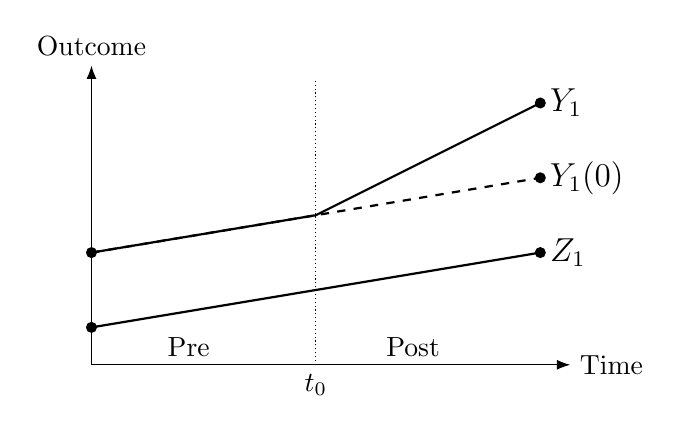
\begin{tikzpicture}[x=0.95cm,y=0.95cm,>=Latex]
    
    % -----------------------
    % Axes
    % -----------------------
    \draw[->] (0,0) -- (6.4,0) node[right] {Time};
    \draw[->] (0,0) -- (0,4.0) node[above] {Outcome};
    
    % Period labels
    \node[below] at (1.3,0.5) {Pre};
    \node[below] at (4.3,0.5) {Post};
    
    % Intervention time (vertical line)
    \draw[densely dotted] (3,0) -- (3,3.8);
    \node[below] at (3,0) {$t_0$};
    
    % -----------------------
    % Coordinates (choose any reasonable numbers)
    % -----------------------
    % Control: pre -> post
    \coordinate (Cpre)  at (0,0.5);
    \coordinate (Cpost) at (6,1.5);
    
    % Treated: observed pre -> observed post
    \coordinate (Tpre)  at (0,1.5);
    \coordinate (Tpost) at (6,3.5);
    
    % NEW: treated value at the intervention time t0 (x=4)
    \coordinate (Tt0)   at (3, 2); % choose y to set the pre-slope
    
    % Treated counterfactual under parallel trends:
    % Tcf = Tpre + (Cpost - Cpre)
    \coordinate (Tcf)   at (6,2.5);
    
    % -----------------------
    % Lines
    % -----------------------
    % Control (solid)
    \draw[thick] (Cpre) -- (Cpost);
    \node[right] at (Cpost) {\large $Z_1$};
    
    % Treated observed (solid)
    \draw[thick] (Tpre) -- (Tt0) -- (Tpost);
    \node[right] at (Tpost) {\large $Y_1$};
    % Treated counterfactual (dashed, parallel to control trend)
    \draw[thick,dashed] (Tpre) -- (Tcf);
    \node[right] at (Tcf) {\large  $Y_1(0)$};
    
    % Points
    \fill (Cpre)  circle (2pt);
    \fill (Cpost) circle (2pt);
    \fill (Tpre)  circle (2pt);
    \fill (Tpost) circle (2pt);
    \fill (Tcf)   circle (2pt);
    
    \end{tikzpicture}
    \end{subfigure}
    \hspace{0.1\textwidth}
    \begin{subfigure}[t]{0.44 \textwidth}
        \raisebox{1.4em}{
        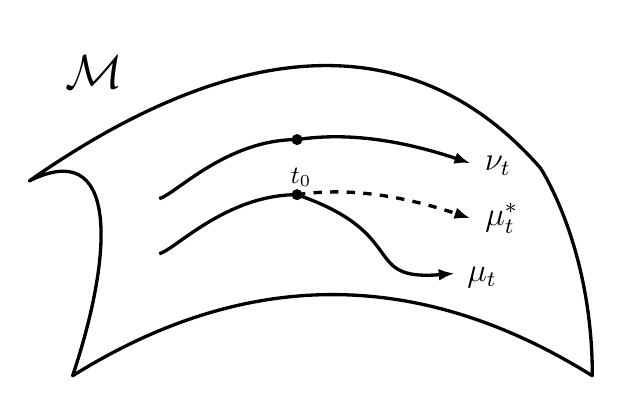
\begin{tikzpicture}[
          scale=1.0,
          >={Latex[length=2.0mm]},
          warp/.style={draw, very thick, line cap=round, line join=round},
          lab/.style={font=\small},
          atom/.style={circle, fill=blue, inner sep=1.6pt},
        ]
        
        % One warped "square-like" manifold + 4 atoms (Diracs)
        \newcommand{\warpsquare}[2]{%
        \begin{scope}[xshift=#1cm,yshift=#2cm, scale=1.1]
          \draw[warp]
            (-3.5, 0.75)
              .. controls (-1.0, 2.5) and ( 1.0, 2.5) .. ( 2.4, 0.9)
              .. controls ( 2.4, 0.9) and ( 3.0,0.0) .. ( 3.0,-1.5)
              .. controls ( 1.0,-0.25) and (-1.0, -0.25) .. (-3.0,-1.5)
              .. controls (-2.5, 0.0) and (-2.5, 1.25) .. (-3.5, 0.75)
            -- cycle;
        
          \node[lab] at (-2.75, 2.0) {\LARGE $\man$};
        \end{scope}
        }
        
        % Two identical manifolds
        \warpsquare{-2}{0}

        % --- Overlay DiD "parallel trends" paths as CURVES on the manifold ---
        \begin{scope}[xshift=-2cm,yshift=0cm]
        
          % A constant shift to create a "parallel" treated pre-trend curve
          % (translation of the entire pre-curve shape)
          \coordinate (Tshift) at (0.0,-0.70);
        
          % -----------------------
          % CONTROL curve: Z_1
          % -----------------------
          % Pre (curved) segment: C0 -> Ct0
          \coordinate (C0)   at (-2.2, 0.60);
          \coordinate (Ct0)  at (-0.45, 1.35);
        
          % Control points chosen to align visually with your warped boundary
          \coordinate (C0c1) at (-2.00, 0.65);
          \coordinate (C0c2) at (-1.35, 1.35);
        
          % Post (curved) segment: Ct0 -> C1
          \coordinate (C1)   at ( 1.75, 1.05);
          \coordinate (C1c1) at (-0.10, 1.40);
          \coordinate (C1c2) at ( 0.55, 1.45);
        
          % Draw control path (curved)
          \draw[very thick, -{Latex[length=2mm]}]
            (C0) .. controls (C0c1) and (C0c2) .. (Ct0)
                 .. controls (C1c1) and (C1c2) .. (C1);
          \node[lab] at (2.10,1.02) {\large $\nu_t$};
        
          % -----------------------
          % TREATED curve: Y_1
          % -----------------------
          % Treated pre endpoints are translated copies of the control pre endpoints.
          \coordinate (T0)  at ($(C0)  + (Tshift)$);
          \coordinate (Tt0) at ($(Ct0) + (Tshift)$);
        
          % Treated observed post endpoint (diverges)
          \coordinate (T1)  at (1.55,-0.35);
        
          % Treated pre control points are also translated (this enforces "parallel" pre-trend)
          \coordinate (T0c1) at ($(C0c1) + (Tshift)$);
          \coordinate (T0c2) at ($(C0c2) + (Tshift)$);
        
          % Draw treated observed path: curved pre (parallel) then diverging curved post
          \draw[very thick, -{Latex[length=2mm]}]
            (T0) .. controls (T0c1) and (T0c2) .. (Tt0)
                .. controls (1.00, 0.15) and (0.35,-0.45) .. (T1);
          \node[lab] at (1.90,-0.4) {\large $\mu_t$};
        
          % -----------------------
          % TREATED counterfactual: Y_1(0)
          % -----------------------
          % Counterfactual post curve is a translated copy of the control post curve.
          \coordinate (Tcf)  at ($(C1)  + (Tshift)$);
          \coordinate (T1c1) at ($(C1c1)+ (Tshift)$);
          \coordinate (T1c2) at ($(C1c2)+ (Tshift)$);
        
          \draw[very thick, dashed, -{Latex[length=2mm]}]
            (Tt0) .. controls (T1c1) and (T1c2) .. (Tcf);
          \node[lab] at ($(Tcf)+(0.4,0.00)$) {\large  $\mu_t^*$};
        
          % Mark t0 points and label t0
          \fill (Ct0) circle (2pt);
          \fill (Tt0) circle (2pt);
          \node[lab] at ($(Ct0)+(0.05,-0.48)$) {$t_0$};
        
        \end{scope}
        
        
        \end{tikzpicture}
        }
    \end{subfigure}
  \vspace{0.5em} % whitespace below the diagram (adjust as needed)
  \caption{Difference-in-differences diagram illustrating the parallel trends assumption in the Euclidean case (left) and the pseudo-Riemannian case (right).}
  \label{fig:did-parallel-trends}
\end{figure}


In many cases, we care about the laws of $Y_t$ and $Z_t$, which we will denote $\mu_t$ and $\nu_t$, as opposed to statistics like their expected value. Unfortunately, since $\mu_t$ and $\nu_t$ are elements of the space of probability measures over $\mathbb{R}^d$, we don't have the abelian structure needed to take \say{differences} as needed in the Difference-in-Differences framework. As a result, we propose a conceptual framework that allows for Difference-in-Differences where population objects that do not live in a Euclidean or vector space. We also instantiate this idea through a procedure that emulates Difference-in-Differences on the space of probability measures over $\mathbb{R}^d$, $\mathcal{P}_2(\mathbb{R}^d)$ equipped with the 2-Wasserstein distance -- we do this by reconstructing the counterfactual trajectory of the \textit{law} of $Y_i(0)$ and using tools from Wasserstein geometry to analyze the difference between the counterfactual law and the treated law. We also propose an analogous method that allows for population \textit{growth} and \textit{decay} by performing counterfactual trajectory reconstruction on the space of nonnegative measures $\mathfrak{M}_+(\mathbb{R}^d)$ equipped with the Hellinger-Kantorovich metric HK. 

We consider the setting where the population-level treated, untreated and control objects can be represented by trajectories through a (potentially infinite-dimensional) pseudo-Riemannian manifold $\man$ equipped with a metric $g$ and a connection $\nabla^{(\man)}$. We denote $(\mu_t)_{t \in [0,1]}$ the path corresponding to the treated population, $(\nu_t)_{t\in [0,1]}$ the path corresponding to the untreated population, and $(\mu_t^*)_{t \in [0,1]}$ the path corresponding to the counterfactual treated population. Our goal is to emulate the Difference-in-Differences procedure and reconstruct the population counterfactual trajectory $(\mu_t^*)_{t \in [0,1]}$ given the control and treated trajectories. 

In order for the counterfactual trajectory to be recoverable, we need an assumption analogous to the parallel trends assumption in Euclidean Differences-in-Differences. Since we are not considering objects living in a vector space, we have no notion of taking differences. Instead we will appeal to Riemannian geometry by using \textit{parallel transport}. Let $\dot \nu_t$ and $\dot \mu_t^*$ be the time derivative of the curves $\mu_t$ and $\nu_t$. Further let $\mathcal{T}_{\nu_t \rightarrow \mu_t^*}(v)$ denote the parallel transport of $v \in T_{\nu_t}(\man)$ along the geodesic connecting $\nu_t$ and $\mu_t^*$.

\begin{restatable}[Pseudo-Riemannian Parallel Trends]{asmpt}{} \label{riemannian parallel trends}
    We assume that the trajectories $(\nu_t)_{t\in [0, 1]}$ and $(\mu_t^*)_{t\in [0, 1]}$ are parallel in at least one of the two following senses.
    \begin{enumerate}
        \item (Parallel velocities): The velocities $\dot \nu_t$ and $\dot \mu_t^*$ are parallel with respect to the connection $\nabla^{(\man)}$ in the sense that $\dot \mu_t^* = \mathcal{T}_{\nu_t \rightarrow \mu_t^*}(\dot \nu_t)$.
        \item (Constant displacement): The displacement between $\nu_t$ and $\mu_t^*$, formally described by $\log^\man_{\nu_t}(\mu_t^*)$, is constant with respect to the connection $\nabla^{(\man)}$, i.e.
        \[\nabla^{(\man)}_{\dot \nu_t}\left(\log^\man_{\nu_t}(\mu_t^*)\right) = 0.\]
        Put differently, it holds that
        \[\mathcal{T}_{\nu_t \rightarrow \nu_{t+s}}\left(\log^\man_{\nu_t}(\mu_{t}^*)\right) = \log^\man_{\nu_{t+s}}(\mu_{t+s}^*).\]
    \end{enumerate}
\end{restatable}
We formalize the \textit{generalized} parallel trends assumption in \Cref{riemannian parallel trends}, and we provide a visualization in \Cref{fig:did-parallel-trends}. Note that we only require one of the two conditions to hold, despite the fact that the parallel trends assumption in the original Difference-in-Differences framework contains both. This is because, in general, properties 1 and 2 of \Cref{riemannian parallel trends} do not coincide if $\man$ has nonzero curvature. In the original Difference-in-Differences framework over Euclidean space, however, the parallel trends assumption gives both properties 1 and 2. We also emphasize that when one takes $\man = \mathbb{R}^d$, we recover the classical parallel trends assumption. In the remainder of this work we focus on part 1 of the assumption, and we leave a more detailed exploration of part 2 to future work.

\subsection{Reconstructing Counterfactual Dynamics with Parallel Transport}

\begin{algorithm}[H]
    \begin{algorithmic}[1]
        \caption{Population counterfactual trajectory reconstruction on $(\mathcal{P}_{2}(\mathbb{R}^d), W_2)$}
        \label{alg: W trajectory reconstruction}
        \Require Absolutely continuous control trajectory $(\nu_i)_{i \in \{1, \dots, T\}}$, treated initial condition $\mu_1 \in \mathcal{P}_2(\mathbb{R}^d)$, approximation resolution $n$. 
        
        \State Initialize counterfactual trajectory $\mu_1^n = \mu_1$. 
        \For{$i = 1$ to $T-1$}
            \State Compute Brenier map $T_{\nu_i \rightarrow \nu_{i+1}}$ and initial velocity $v^{(i)} = (T_{\nu_i \rightarrow \nu_{i+1}} - I_d)$.
            \State Compute the Brenier map $T_{\nu_i \rightarrow \mu_i^*}$ and stepsize $s = W_2(\nu_i, \mu_i^*)/n.$
            \State Set $v^{(i)}_1 = v^{(i)}$.
            \State Compute the maps $F_k^{(i)} = (1 - \frac{k}{n})I_d + \frac{k}{n}T_{\nu_i \rightarrow \mu_i^*}$ for $k \in \{1, \dots, n\}$.
            \For{$k = 1$ to $n-1$}
                \State Compute the interpolated measure $\tilde\mu_k^{(i)} = (F_{k}^{(i)})_\#\nu_i$.
                \State Set $j_{(x, \cdot)}(0, v_k^{(i)}(x))(s) = sv_k^{(i)}(x)$, the solution to the Jacobi equation on $\mathbb{R}^d$.
                \State Define the step map $S_k^{(i)} = F_{k+1}^{(i)} \circ (F_{k}^{(i)})^{-1}.$
                \State Compute $v_{k+1}^{(i)} = \Pi_{\tilde\mu_{k+1}^{(i)}}\left(s^{-1}j(0, v_k^{(i)})(s) \circ (S_k^{(i)})^{-1}\right) = \Pi_{\tilde\mu_{k + 1}^{(i)}}(v_k^{(i)} \circ (S_k^{(i)})^{-1})$. 
            \EndFor
            \State Set $v^{(i+1)} = v^{(i)}_n$.
            \State Reconstruct $\mu^n_{i+1} = (I_d + v^{(i+1)})_\#\mu_i^n$.
        \EndFor
    \State \Return counterfactual trajectory $(\mu_i^n)_{i \in \{1, \dots, T\}}$.
    \end{algorithmic}
\end{algorithm} 

\begin{restatable}{asmpt}{} \label{all necessary W assumptions}
    We assume that the measures $(\nu_i)_{i \in \{1, \dots, T\}}$ and $(\mu_i^*)_{i \in [1, \dots, T]}$ are all absolutely continuous. Furthermore, we require that they satisfy the following conditions. For all $i$,
    \begin{enumerate}
        \item $\nu_{i}$ and $\nu_{i+1}$ can be connected by a regular $W_2$ geodesic.
        \item $\nu_i$ and $\mu_i^*$ can be connected by a regular $W_2$ geodesic.
    \end{enumerate}
    \tls{Need to flesh this out}
\end{restatable}

\begin{restatable}[One step error of \Cref{alg: W trajectory reconstruction}]{lemma}{}
    Let $\nu_i, \nu_{i+1}, \mu_i^* \in \mathcal{P}_2(\mathbb{R}^d)$ be absolutely continuous measures and suppose there exists a tangent vector $\nabla\varphi_i \in T_{\nu_i}\mathcal{P}_2(\mathbb{R}^d)$ such that $\mathbf{exp}_{\nu_i}(\nabla\varphi_i) = \nu_{i+1}.$ Further let $\nabla \varphi^*_i$ be the parallel transport of $\nabla\varphi_i$ along the Wasserstein geodesic connecting $\nu_i$ and $\mu_i^*$, and let $\mu_{i+1}^* = \mathbf{exp}_{\mu_i^*}(\nabla\varphi^*_i)$. If $\nabla\varphi_i^*$ is spatially Lipschitz, then,
    \[W_2(\mu_{i+1}^n, \mu_{i+1}^*) \lesssim  W_2(\mu_{i}^n, \mu_i^*) + O\left(\frac{1}{n}\right).\]
\end{restatable}
\noindent \textit{Proof.} Let $\tilde\mu_i \triangleq (I_d + v_n)_\# \mu_i^*$. We have 
\begin{align*}
    W_2(\mu_{i+1}^n, \mu_{i+1}^*) &= W_2((I_d + v^n)_\#\mu_i^n, (I_d + \nabla\varphi_i^*)_\#\mu_i^*) \\
    &\leq W_2((I_d + v^n)_\#\mu_i^n, (I_d + \nabla\varphi_i^*)_\#\mu_i^n) + W_2((I_d + \nabla\varphi_i^*)_\#\mu_i^n, (I_d + \nabla \varphi_i^*)_\#\mu_i^*).
\end{align*}
For the second term, let $\gamma^*$ denote the optimal coupling of $\mu_i^n$ and $\mu_i^*$. We can upper bound the Wasserstein distance between the pushforwards $(I_d + \nabla\varphi_i^*)_\# \mu_i^n$ and $(I_d + \nabla\varphi_i^*)_\#\mu_i^*$ using $\gamma^*$ as follows,
\begin{align*}
    W_2^2((I_d + \nabla\varphi_i^*)_\#\mu_i^n, (I_d + \nabla\varphi_i^*)_\#\mu_i^*) &\leq \int_{\mathbb{R}^d \times\mathbb{R}^d} \|x - y + \nabla\varphi_i^*(x) - \nabla\varphi_i^*(y)\|_2^2\, d\gamma^*(x,y) \\
    &\lesssim  W_2^2(\mu_i^n, \mu_i^*) + \int_{\mathbb{R}^d \times\mathbb{R}^d} \|\nabla\varphi_i^*(x) - \nabla\varphi_i^*(y)\|_2^2\, d\gamma^*(x,y) \\
    &\leq (1 + \text{L}(\nabla\varphi_i^*))^2W_2^2(\mu_i^n, \mu_i^*).
\end{align*}
For the first term, consider the suboptimal coupling of the pushforwards given by $((I_d + v^n)(X), (I_d + \nabla\varphi_i^*)(X))$ where $X \sim \mu_i^n$. Then we have
\begin{align*}
    W_2^2((I_d + v^n)_\#\mu_i^n, (I_d + \nabla\varphi_i^*)_\#\mu_i^n) &\leq \int_{\mathbb{R}^d\times \mathbb{R}^d}\|x + v^n(x) - x - \nabla\varphi_i^*(x)\|_2^2 \, d\mu_i^n \\
    &= \|v^n - \nabla\varphi_i^*\|_{L_2(\mu_i^n)}^2.
\end{align*}
Applying \Cref{full approximation of parallel transport along regular curves} concludes the proof. \qed{}

\begin{restatable}{thm}{}
    Consider the regime described in \Cref{all necessary W assumptions} and let $\hat{\mu}_i^* \triangleq \mu_i^n$. Then we have the following accumulated error bound on the counterfactual trajectory,
    \[\sum_{i = 1}^TW_2(\hat{\mu}_i^*, \mu_i^*) = O\left(\frac{T}{n}\right).\]
    In the setting where $T = \Theta(1)$ and $n \rightarrow \infty$, the accumulated error is $o(1)$. 
\end{restatable}


\begin{algorithm}[H]
    \begin{algorithmic}[1] 
        \caption{Population counterfactual trajectory reconstruction on $(\mathfrak{M}_+(\Omega), \text{HK})$}
        \label{alg: HK trajectory reconstruction}
        \Require Absolutely continuous control trajectory $(\nu_i)_{i \in \{1, \dots, T\}}$, treated initial condition $\mu_1 \in \mathfrak{M}_+(\Omega)$, approximation resolution $n$, restriction parameter $\varepsilon > 0$. 
        \State Set geodesic interpolant map on $\mathfrak{C}_\Omega$, $Z_t(z_0, z_1) = Z(t; z_0, z_1)$.
        \State Initialize counterfactual trajectory $\mu_1^{\varepsilon, n} \triangleq \mu_1 = \mu_1^*$. 
        \For{$i = 1$ to $T-1$}
            \State Compute optimal lifts $\lambda_{i}, \lambda_{i+1}$ = LiftToCone($\nu_i$, $\nu_{i+1}$) and coupling $\pi^*_{i, i+1} \in \mathcal{P}_2(\mathfrak{C}_{\Omega} \times \mathfrak{C}_{\Omega})$. 
            \State Clip endpoints, $\lambda^{\varepsilon}_{i, i+1} = (Z_\varepsilon)_\#\pi^*_{i, i+1}$, $\lambda^{1 - \varepsilon}_{i, i+1} = (Z_{1-\varepsilon})_\#\pi^*_{i, i+1}$.
            \State Compute Monge map $T_{i, i+1}$ s.t. $(T_{i, i+1})_\#\lambda^{\varepsilon}_{i, i+1} = \lambda^{1-\varepsilon}_{i, i+1}$ and tangent $V^\varepsilon_{i, 0} = \log ^{\mathfrak{C}}(T_{i, i+1})$. 
            \State Compute optimal lifts $\lambda_{\nu_{i}}$, $\lambda_{\mu^{\varepsilon, n}_{i}}$ = LiftToCone($\nu_i$, $\mu_{i}^{\varepsilon, n}$).
            \State Compute optimal coupling $\pi^*_{(i)} \in \mathcal{P}_2(\mathfrak{C}_{\Omega} \times \mathfrak{C}_{\Omega})$ and stepsize $s_{(i)} = (1-2\varepsilon)W_\mathfrak{C}(\lambda_{\nu_{i}}, \lambda_{\mu_{i}^{\varepsilon, n}})/n$. 
            \State Clip endpoints, $\lambda^{\varepsilon}_i = (Z_\varepsilon)_\#\pi^*_{(i)}$, $\lambda_{i}^{1-\varepsilon} = (Z_{1-\varepsilon})_\#\pi^*_{(i)}$ and set $\lambda_{i, 0}^\varepsilon = \lambda_i^{\varepsilon}$.
            \State Obtain Monge map $T^{(i)}$ pushing $ \lambda^{\varepsilon}_{i}$ to $\lambda^{1-\varepsilon}_{i}$ and the log map $u^{(i)}_0 = \overline{\log}^\mathfrak{C}(T^{(i)})$.
            \State Compute interpolation maps $F_k^{(i)} = \exp^{\mathfrak{C}}(s_{(i)}ku_0^{(i)})$ for $k \in \{0, \dots, n\}$.
            \For{$k = 1$ to $n$}
                \State Compute the step map $S_k^{(i)} = F_k^{(i)} \circ (F_{k-1}^{(i)})^{-1}$ and the log map $u_k^{(i)} = \overline{\log}^{\mathfrak{C}}(S_k^{(i)})$.
                \State Compute the interpolated measure $\lambda_{i, k}^{\varepsilon} = (S_{k}^{(i)})_\# \lambda_{i, k-1}^{\varepsilon}$.
                \State Compute $\left(z \mapsto j_{z, u_k^{(i)}}(0, V_{i, k-1}^\varepsilon(z))(s_{(i)})\right)$ the Jacobi field evaluated at $s_{(i)}$ with initial \hspace*{\algorithmicindent}\hspace*{\algorithmicindent}conditions $0$ and $V^\varepsilon_{i, k-1}$, and parallel transport approximation
                \[V_{i, k}^\varepsilon = \Pi_{\lambda_{i, k}^\varepsilon}\left(s_{(i)}^{-1}j_{z, u_k^{(i)}}(0, V_{i, k-1}^\varepsilon(z))(s_{(i)}) \circ (S_k^{(i)})^{-1}\right).\]
                
            \EndFor
            \State Reconstruct $\mu_{i + 1}^{\varepsilon, n} = \mathbf{exp}_{\mu_i^{\varepsilon, n}}^{\text{HK}}(\mathcal{P}_{\lambda_i^{1-\varepsilon}}(V_{i, n}^\varepsilon))$\Comment{\Cref{HK exponential map closed form}}
        \EndFor
    \State \Return predicted counterfactual trajectory $(\mu_i^{\varepsilon, n})_{i \in \{1, \dots, T\}}$.
    \end{algorithmic}
\end{algorithm} 

\begin{restatable}{asmpt}{} \label{all necessary HK assumptions}
    We assume that the measures $(\nu_i)_{i \in \{1, \dots, T\}}$ and $(\mu_i^*)_{i \in [1, \dots, T]}$ are all supported on $\Omega \subset \subset \mathbb{R}^d$ where $\text{diam}(\Omega) < \pi/2$. Furthermore, we require that they satisfy the following conditions:
    \begin{enumerate}
        \item For all $i$, $\nu_{i}$ and $\nu_{i+1}$ can be connected by a HK geodesic with tangent velocity field given by $(\nabla\varphi_t, \varphi_t)_{t \in [0, 1]}$ such that $\|\nabla^2\varphi\|_{L_\infty(\Omega)}, $
    \end{enumerate}
    \tls{Need to flesh this out}
\end{restatable}

\begin{restatable}[One step error of \Cref{alg: HK trajectory reconstruction}]{lemma}{} \label{HK trajectory consistency}
    Let $\nu_{i}, \nu_{i+1}, \mu_i^* \in \mathfrak{M}_+(\Omega)$ be absolutely continuous and have density bounded away from zero on $\Omega$, and suppose that there exists a tangent vector $\mathbf{v}_i \triangleq (\nabla \varphi_i, \varphi_i) \in T_{\nu_i}\mathfrak{M}_+(\Omega)$ such that $\mathbf{exp}_{\nu_i}(\mathbf{v}_i) = \nu_{i+1}$. Further let $\mathbf{v}_i^* \in T_{\mu_i^*}\mathfrak{M}_+(\Omega)$ be the parallel transport of $\mathbf{v}_i$ along the HK geodesic connecting $\nu_i$ and $\mu_i^*$, and let $\mu_{i+1}^* = \mathbf{exp}_{\mu_i^*}(\mathbf{v}_i^*)$. Then we have
    \[\text{HK}(\mu_{i+ 1}^{\varepsilon, n}, \mu_{i + 1}^*) \leq \text{L}^{\text{base}}(\mathbf{exp})\cdot\text{HK}(\mu_{i}^{\varepsilon, n}, \mu_i^*) + O\left(\frac{1}{n} \vee\frac{e^{2K/\varepsilon}}{\varepsilon^2n^3} + \varepsilon\right)\]
    where $\text{L}^{\text{base}}(\mathbf{exp})$ is the Lipschitz constant of the HK exponential map in its base argument.
\end{restatable}

\begin{restatable}{thm}{}
    Consider the regime described by \Cref{all necessary HK assumptions} and let $\hat\mu_{i}^* \triangleq \mu_{i}^{\varepsilon, n}$. Then we have the following accumulated error bound on the counterfactual trajectory
    \[\sum_{i = 1}^T\text{HK}(\hat{\mu}_i^*, \mu_i^*) = O\left(\frac{T}{n} \vee\frac{Te^{2K/\varepsilon}}{\varepsilon^2n^3} + T\varepsilon\right).\]
    Moreover, if $T = \Theta(1)$, $n \rightarrow \infty$, $\varepsilon \rightarrow 0$ and $n\varepsilon e^{-K/\varepsilon} \rightarrow \infty$, then the right hand side of the panel above is $o(1)$. 
\end{restatable}
\noindent \textit{Proof.} Let $i \in \{2, \dots, T\}$. By \Cref{HK trajectory consistency} we have
\begin{align*}
    \text{HK}(\hat{\mu}_i^*, \mu_i^*) \lesssim \text{HK}(\hat\mu_{i-1}^*, \mu_{i-1}^*) + O\left(\frac{1}{n} \vee\frac{e^{2K/\varepsilon}}{\varepsilon^2n^3} + \varepsilon\right) &\lesssim \sum_{i = 1}^TO\left(\frac{1}{n} \vee\frac{e^{2K/\varepsilon}}{\varepsilon^2n^3} + \varepsilon\right)\\ &= O\left(\frac{T}{n} \vee\frac{Te^{2K/\varepsilon}}{\varepsilon^2n^3} + T\varepsilon\right).
\end{align*} \qed{}

\appendix

\section{Proofs} \label{sec: proof of main results}

\noindent \textbf{Proof of \Cref{cone exponential and log map}.} We desire a $z_1 \in \mathfrak{C}_\Omega$ such that $Z'(0^+; z_0, z_1)$, the right derivative at $0$, is equal to $(v_x, v_r).$ Letting $\theta = \|x_1 - x_0\|_2$, one can verify that 
\begin{align*}
    \rho'(s; z_0, z_1) = \frac{\sin^2(\theta)r_0r_1^2s}{\theta B(s)^{3/2}\sqrt{1 - \frac{A(s)^2}{B(s)}}}
\end{align*}
with 
\begin{equation*}
    A(s) = r_1s\cos(\theta) + r_0(1-s) \qquad B(s) = r_1^2s^2 + 2s(1-s)r_0r_1\cos(\theta) + r_0^2(1-s)^2.
\end{equation*}
We can directly evaluate $\lim_{s \rightarrow 0^+}B(s) = r_0^2$. For the radical,
\begin{align*}
    1 - \frac{A(s)^2}{B(s)} = \frac{\left(\frac{r_1s}{r_0(1-s)}\right)^2\sin^2(\theta)}{1 + 2\frac{r_1s}{r_0(1-s)}\cos(\theta) + \left(\frac{r_1s}{r_0(1-s)}\right)^2} = \left(\frac{r_1s}{r_0(1-s)}\right)^2\sin^2(\theta)\left(1 + u - u^2 + O(u^3)\right)
\end{align*}
where $u = 2\frac{r_1s}{r_0(1-s)}\cos(\theta) + \left(\frac{r_1s}{r_0(1-s)}\right)^2$. Plugging back in and canceling terms yields
\begin{align*}
    \lim_{s \rightarrow 0^+}\rho'(s; z_0, z_1) = \lim_{s\rightarrow 0^+}\left(\frac{\sin(\theta)r_1r_0^2(1-s)}{\theta B(s)^{3/2}\sqrt{1  + u - u^2 + O(u^3)}}\right) = \frac{\sin(\theta)r_1}{\theta r_0}
\end{align*}
since $\lim_{s \rightarrow 0^+}u = 0$, which implies $X'(0^+; z_0, z_1) = \frac{\sin(\theta)r_1(x_1 - x_0)}{\theta r_0}$. One can also easily verify that $R(0^+; z_0, z_1) = r_1\cos(\theta) - r_0$. Now we have a system of equations 
\begin{equation*}
    v_x = \frac{\sin(\|x_1 - x_0\|_2)r_1(x_1 - x_0)}{\|x_1 - x_0\|_2 r_0} \quad \text{and} \quad  v_r = r_1\cos(\|x_1 - x_0\|_2) - r_0
\end{equation*}
for which we know $(x_0, r_0)$ and we want to solve for $(x_1, r_1)$. One can verify that the solution is $r_1 = \sqrt{\|v_x\|_2^2r_0 + (v_r+r_0)^2}$ and $x_1 = x_0 + \theta\frac{v_x}{\|v_x\|_2}$ with $\theta = \text{atan2}(r_0\|v_x\|_2, v_r + r_0) \in [0, \pi)$. This completes the exponential map. The logarithmic map is given by
$\log^{\mathfrak{C}}_{z_1}(z_0) = Z'(0^+; z_0, z_1)$, the expressions for which we have already derived in computing the exponential map.
\qed{}
\\

\noindent \textbf{Proof of \Cref{one step parallel transport approx result}.} Let $\mathbf{T}(t, s, \cdot)$ be the flow map of the regular curve $\nu_s$ and let $V \in L_2(\nu_s).$ We'll define the following function, 
\begin{equation*}
    \tau_{t_0}^{t_1}(V)(x) \triangleq \begin{cases}
        \text{the parallel transport of $V(\mathbf{T}(t_1, t_0, x))$ on $\man$ along the curve} \\
        r \mapsto \mathbf{T}(t_1, r, x) \text{ from $r = t_0$ to $r = t_1$ }.
    \end{cases}
\end{equation*}
By the triangle inequality, we have
\begin{align*}
    \|w_s - \mathcal{T}_0^s(v)\|_{L_2(\nu_s)} \leq \|w_s - \Pi_{\nu_s}(\tau_0^s(v)\circ F^{-1}_s)\|_{L_2(\nu_s)} + \|\Pi_{\nu_s}(\tau_0^s(v)\circ F^{-1}_s) - \mathcal{T}_0^s(v)\|_{L_2(\nu_s)}.
\end{align*}
By equations 4.18 and 4.10 of \citet{gigli2012second}, we have that the second term satisfies
\begin{align*}
    \|\Pi_{\nu_s}(\tau_0^s(v)\circ F^{-1}_s) - \mathcal{T}_0^s(v)\|_{L_2(\nu_s)} \leq \left(e^{\int_0^1\text{L}(\nabla \psi_r)dr} - 1\right)^2\|v\|_{L_2(\mu)}\left(\int_0^s\text{L}(\nabla\psi_r)dr\right)^2
\end{align*}
$\text{L}(\nabla\psi_r)$ is the largest Lipschitz constant of the velocity field generating the geodesic $\mathbf{exp}_{\mu}(su).$ Now we will handle the first term in the triangle inequality. Note that $\Pi_{\nu_s}: L_2(\nu_s) \rightarrow T_{\nu_s}\mathcal{P}_{2}(\man)$ is a projection onto a closed and linear subset, and it is therefore non-expansive. This allows us to say
\begin{align*}
    \|w_s - \Pi_{\nu_s}(\tau_0^s(v)\circ F^{-1}_s)\|_{L_2(\nu_s)} &\leq \left\|s^{-1}j_{\mu, u}\left(0, v\right)(s)  - \tau_0^s(v) \circ F^{-1}_s \right\|_{L_2(\nu_s)} \\
    &= \left(\int \|s^{-1}j_{F_s^{-1}(y), u(F_s^{-1}(y))}\left(0, v(F_s^{-1}(y))\right)(s)  - \tau_0^s(v)(F_s^{-1}(y))\|_g^2 \,d\nu_s\right)^{1/2} \\
    &= \left(\int \|s^{-1}j_{x, u(x)}\left(0, v(x)\right)(s)  - \tau_0^s(v)(x) \|_g^2 \,d\mu\right)^{1/2}.
\end{align*}
Now we'll apply \Cref{fanning approximation} to say 
\begin{align*}
    \|s^{-1}j_{x, u(x)}\left(0, v(x)\right)(s)  - \tau_0^s(v)(x)\|_g \leq As^2\|v\|_g
\end{align*}
for $s$ sufficiently small, which implies 
\begin{align*}
    \|w_s - \Pi_{\nu_s}(\tau_0^s(v)\circ F^{-1}_s)\|_{L_2(\nu_s)} &\leq \left(\int A^2s^4\|v(x)\|_g^2 \,d\mu\right)^{1/2}  = As^2\|v\|_{L_2(\mu)}.
\end{align*}
The second part of the thesis follows from the fact that $s \mapsto \nu_s$ is regular and thus admits a velocity field with an spatial Lipschitz constant that integrates to $O(s)$ where $s$ is the length of the interval of integration.
\qed{}
\\

\noindent \textbf{Proof of \Cref{full approximation of parallel transport along regular curves}.} By \Cref{one step parallel transport approx result} we know that for each $k \in \{1\, \dots , n\}$ we have $\|\mathcal{P}_k(w) - \mathcal{T}_k(w)\|_{L_2(\nu_{ks})} = Cs^2\|w\|_{L_2(\nu_{ks})}$ for some $C > 0$ independent of $k$. Now let $e_k \triangleq v^{\text{approx}}_k - v^{\text{exact}}_k.$ By the triangle inequality
\begin{align*}
    \|v^{\text{approx}}_k - v^{\text{exact}}_k\|_{L_2(\nu_{sk})}  &= \|\mathcal{P}_k(v_{k-1}^{\text{approx}}) - \mathcal{T}_k(v_{k-1}^{\text{exact}})\|_{L_2(\nu_{sk})}\\ &\leq \|\mathcal{P}_k(v_{k-1}^{\text{approx}}) - \mathcal{T}_k(v_{k-1}^{\text{approx}})\|_{L_2(\nu_{sk})} + \|\mathcal{T}_k(v_{k-1}^{\text{approx}}) - \mathcal{T}_k(v_{k-1}^{\text{exact}})\|_{L_2(\nu_{sk})}.
\end{align*}
Note that the first term is bounded by $Cs^2\|v^{\text{approx}}_{k - 1}\|_{L_2(\nu_{(k-1)s})}$. Since parallel transport is an isometry, we have that the second term can be rewritten to
\[\|\mathcal{T}_k(v_{k-1}^{\text{approx}}) - \mathcal{T}_k(v_{k-1}^{\text{exact}})\|_{L_2(\nu_{sk})} = \|v_{k-1}^{\text{approx}} - v_{k-1}^{\text{exact}}\|_{L_2(\nu_{s(k-1)})} = \|e_{k-1}\|_{L_2(\nu_{s(k-1)})}.\]
Putting it together, we have the recurrence relation 
\[\|e_k\|_{L_2(\nu_{sk})} \leq Cs^2\|v^{\text{approx}}_{k - 1}\|_{L_2(\nu_{(k-1)s})} + \|e_{k-1}\|_{L_2(\nu_{s(k-1)})}.\]
By a similar argument, we can say $\|v_{k-1}^{\text{approx}}\|_{L_2(\nu_{(k-1)s)}} \leq \|v\|_{L_2(\mu)} + \|e_{k-1}\|_{L_2(\nu_{s(k-1)})}$ which implies 
\[\|e_k\|_{L_2(\nu_{sk})} \leq Cs^2\|v\|_{L_2(\mu)} + \|e_{k-1}\|_{L_2(\nu_{s(k-1)})}\left( 1 + Cs^2\right).\]
One can verify that the recurrence relation implies
\begin{multline} \label{eq: error recursion}
\|e_k\|_{L_2(\nu_{sk})} \leq Cs^2\|v\|_{L_2(\mu)}\sum_{i = 0}^k(1 + Cs^2)^i\\ = Cs^2\|v\|_{L_2(\mu)} \frac{(1 + Cs^2)^{k} - 1}{Cs^2} = \|v\|_{L_2(\mu)}\left((1 + Cs^2)^{k} - 1\right).\end{multline}
Since $k \leq n = 1/s$ it holds that $(1 + Cs^2)^k \leq (1 + Cs^2)^{1/s}  = 1 + Cs + O(s^2)$. It follows that $\|e_k\|_{L_2(\nu_{sk})} = O(s)$
for all $k \leq n$. 
\qed{}
\\

\noindent \textbf{Proof of \Cref{parallel transport approx entire geodesic clipped}.} Recall the explicit bound from \Cref{one step parallel transport approx result}
\begin{align*}
    \|\mathcal{P}_k(v) - \mathcal{T}_k(v)\|_{L_2(\nu_{ks})} \leq As^2\|v\|_{L_2(\nu_{(k-1)s})} + \left(e^{\left(\int_\varepsilon^{1-\varepsilon}\text{L}(\nabla \psi_r)dr\right)}  - 1\right)^2\|v\|_{L_2(\nu_{(k-1)s})}\left(\int_{(k-1)s}^{ks}\text{L}(\nabla\psi_r)dr\right)^2.
\end{align*}
Corollary 2.16 of \citet{gigli2012second} indicates that the spatial Lipschitz constant of the velocity field generating a $\varepsilon$-restricted geodesic in $\mathcal{P}_2(\man)$ is $\text{L}(\nabla \psi_r) \lesssim 1/\varepsilon$. It follows that 
\[\int_{\varepsilon}^{1-\varepsilon}\text{L}(\nabla \psi_r)dr \leq \frac{K}{\varepsilon} \quad \text{and} \quad \left(\int_{(k-1)s}^{ks}\text{L}(\nabla\psi_r)dr\right)^2 \leq \frac{K^2s^2}{\varepsilon^2}\]
for some $K > 0$ constant which implies 
\begin{align*}
    \|\mathcal{P}_k(v) - \mathcal{T}_k(v)\|_{L_2(\nu_{ks})} \leq \left(A +\frac{e^{2K/\varepsilon}K^2s^2}{\varepsilon^2}\right)s^2\|v\|_{L_2(\nu_{(k-1)s})} \lesssim  s^2 \vee\frac{e^{2K/\varepsilon}s^4}{\varepsilon^2}.
\end{align*}
Now if we apply the same argument as that of \Cref{full approximation of parallel transport along regular curves} we see that 
\begin{align*}
    \|v_n^{\text{approx}} - v_n^{\text{exact}}\|_{L_2(\nu)} = O\left(s \vee\frac{e^{2K/\varepsilon}s^3}{\varepsilon^2}\right).
\end{align*}
Thus, if  $s \geq e^{2K/\varepsilon}s^3/\varepsilon^2$, or equivalently, if 
\[n \gtrsim \frac{e^{K/\varepsilon}}{\varepsilon}\]
then $\|v_n^{\text{approx}} - v_n^{\text{exact}}\|_{L_2(\nu)} = o(1).$ \qed{}
\\

\noindent \textbf{Proof of \Cref{isometry}.} We will start by showing that 
\[\mathcal{L}_{\mathfrak{B}\lambda, \lambda}: L_2(\mathfrak{B}\lambda; \Omega) \times L_2(\mathfrak{B}\lambda) \rightarrow L_2(\lambda; \mathfrak{C}_\Omega) \quad \text{given by} \quad \mathcal{L}_{\mu, \lambda}[(v, \beta)](x,r) = (v(x), 2\beta(x)r)\]
is an isometry. Let $s_1 = (v_1, \beta_1)$ and $s_2 = (v_2, \beta_2)$ be elements of $L_2(\mathfrak{B}\lambda; \Omega) \times L_2(\mathfrak{B}\lambda)$. Their inner product in the domain Hilbert space is given by 
\[\langle s_1, s_2\rangle_{\mathfrak{B}\lambda} = \int_{\Omega}\left( \langle v_1(x), v_2(x)\rangle + 4\beta_1(x)\beta_2(x)\right)d\mathfrak{B}\lambda(x) \]
where the inner product $\langle\cdot, \cdot\rangle$ is the standard Euclidean inner product on $\mathbb{R}^d$. For the lifted field, the inner product in the image is given by
\begin{align*}\langle \mathcal{L}[s_1], \mathcal{L}[s_2]\rangle_{\lambda} = \int_{\mathfrak{C}_\Omega} \langle \mathcal{L}[s_1], \mathcal{L}[s_2]\rangle_{\mathfrak{C}} d\lambda &= \int_{\mathfrak{C}_\Omega}r^2\left(4\beta_1(x)\beta_2(x) + \langle v_1(x), v_2(x) \rangle\right)d\lambda(x,r) \\
&= \int_\Omega \left(4\beta_1(x)\beta_2(x) + \langle v_1(x), v_2(x) \rangle\right)d\mathfrak{B}\lambda(x)
\end{align*}
by \Cref{eq: measure projection}. Thus, $\langle \mathcal{L}[s_1], \mathcal{L}[s_2]\rangle_{\lambda} = \langle s_1, s_2\rangle_{\mathfrak{B}\lambda}$ proving (a). Now we will prove (b). Let $u, v \in L_2(\lambda; \mathfrak{C}_\Omega)$ where $u = a + b\partial_r$ and $v = c + d\partial_r$. Their inner product in the domain Hilbert space is given by
\begin{align*}
    \langle u, v\rangle_{\lambda} &= \int_{\mathfrak{C}} \langle u, v \rangle_{\mathfrak{C}}\,d\lambda = \int_{\mathfrak{C}} \left(b(x,r)d(x,r) + r^2\langle a(x,r), c(x,r)\rangle \right)\,d\lambda(x,r)
\end{align*}
where the inner product on the right is the standard Euclidean inner product on $\mathbb{R}^d$. By the hypothesis, the radial law of $\lambda$ is deterministic given $x$. Thus, the projections of $u$ and $v$ are given by $\mathcal{P}_{\lambda}[u](x) = (a(x,r(x)), b(x,r(x))/2r(x))$ and $\mathcal{P}_{\lambda}[v](x) = (c(x,r(x)), d(x,r(x))/2r(x))$ (due to \Cref{deterministic vector projection}) and their inner product is
\begin{align*}
    \langle \mathcal{P}_{\lambda}[u], \mathcal{P}_{\lambda}[v]\rangle_{\mathfrak{B}\lambda} &= \int_{\Omega} \left(\frac{4b(x, r(x))d(x, r(x))}{4r^2(x)} +  \langle a(x, r(x)), c(x,r(x)\rangle\right)d\mathfrak{B\lambda}(x) \\
    &= \int_{\Omega}\left(\frac{b(x, r(x))d(x, r(x))}{r^2(x)} +  \langle a(x, r(x)), c(x,r(x)\rangle\right)d\mathfrak{B\lambda}(x) \\
    &= \int_{\mathfrak{C}_\Omega}\left(b(x, r(x))d(x, r(x)) +  r^2(x)\langle a(x, r(x)), c(x,r(x)\rangle\right)d\lambda(x, r(x))
\end{align*}
which is equivalent to $\langle u, v \rangle_\lambda$. \qed{}
\\

\noindent \textbf{Proof of \Cref{commutator}.} First we need to establish that the radial conditional law of $\lambda_t$ is deterministic for all $t \in [\varepsilon, 1-\varepsilon]$. This renders $\mathcal{P}_{\lambda_t}$ an isometry, ensuring that it commutes with parallel transport. Under the hypotheses listed, we know that $\lambda_0$ and $\lambda_1$ have a deterministic conditional radial law and their optimal coupling is supported on a map (\Cref{clancy coupling supported on a map}) given by
\[(x_0, r_0(x_0)) \mapsto (T(x_0), r_1(T(x_0)).\]
The interpolated measures $\lambda_t$ therefore can be expressed by 
\[\lambda_t = (z_t)_\#\lambda_{0,x} \quad \text{where}\quad z_t(x_0) = Z_t([x_0, r_0(x_0)], [T(x_0), r_1(T(x_0))])\]
where $\lambda_{0, x}$ is the $x$-marginal of $\lambda_0$. Now let $[X_t(\cdot), R_t(\cdot )]$ be the flow map starting at time $\varepsilon$ described by \Cref{lifting velocities}. On the interior of the Wasserstein geodesic between $\lambda_0$ and $\lambda_1$ we know that the flow map is generated by a spatially Lipschitz velocity field on $\mathfrak{C}_\Omega$ -- by the Cauchy-Lipschitz theorem, this guarantees that the flow ODE admits a unique solution for each initial condition. This property ensures that the flow map is necessarily injective, guaranteeing that $\lambda_t$ can be decomposed as $\lambda_t(dx, dr) = \mu_t(dx)\delta_{r_t(x)}(dr)$ for all $t \in [\varepsilon, 1 - \varepsilon]$ as desired. Thus, by \Cref{isometry} $\mathcal{P}_{\lambda_t}$ is an isometry for all $t \in [\varepsilon, 1 - \varepsilon]$.

Now let $\mathbf{u}_t$ be a parallel vector field along $\mu_t$  where $u = \mathcal{L}[\mathbf{u}_{t_0}]$. Further let $u_t = \mathcal{L}[\mathbf{u}_t]$ be the lifted field along $\lambda_t$. It suffices to show that $u_t$ is the parallel transport along $\lambda_t$, since we have constructed it to project back to $\mathbf{u}_t$. Now let $v_t$ be another vector field along $\lambda_t$. By the metric compatibility of the covariant derivative on $\mathfrak{C}_\Omega$, we have
\[\int_{\mathfrak{C}_\Omega}\frac{d}{dt} \langle v_t, u_t\rangle_{\mathfrak{C}} d\lambda_t = \int_{\mathfrak{C}_\Omega}\langle \nabla^\mathfrak{C}_{\dot \lambda_t} v_t,  u_t\rangle_{\mathfrak{C}} d\lambda_t + \int_{\mathfrak{C}_\Omega} \langle v_t, \nabla^\mathfrak{C}_{\dot \lambda_t}u_t\rangle_{\mathfrak{C}} d\lambda_t.\]
Since we have shown that $\mathcal{P}_{\lambda_t}$ is an isometry, we have that 
\[\int_{\mathfrak{C}}\langle v_t, u_t \rangle_\mathfrak{C} d\lambda_t  = \langle \mathbf{u}_t, \mathcal{P}_{\lambda_t}[u_t] \rangle_{\mu_t}.\]
Differentiating yields,
\begin{align*}
\frac{d}{dt}\int_{\mathfrak{C}}\langle v_t, u_t \rangle_\mathfrak{C} d\lambda_t  &= \frac{d}{dt}\langle \mathcal{P}_{\lambda_t}[v_t], \mathcal{P}_{\lambda_t}[u_t] \rangle_{\mu_t} \\
&= \langle \nabla_{\dot \mu_t}^{\text{HK}}\mathcal{P}_{\lambda_t}[v_t], \mathbf{u}_t \rangle_{\mu_t} + \langle \mathcal{P}_{\lambda_t}[v_t], \underbrace{\nabla_{\dot \mu_t}^{\text{HK}}\mathbf{u}_t}_{0} \rangle_{\mu_t}.
\end{align*}
Using the fact that $\mathcal{L}$ is an isometry (\Cref{isometry}),
\begin{align*}
\frac{d}{dt}\int_{\mathfrak{C}}\langle v_t, u_t \rangle_\mathfrak{C} d\lambda_t  &= \langle \nabla_{\dot \mu_t}^{\text{HK}}\mathcal{P}_{\lambda_t}[v_t], \mathbf{u}_t \rangle_{\mu_t} = \int_{\mathfrak{C}}\left\langle \mathcal{L}[\nabla_{\dot \mu_t}^{\text{HK}}\mathcal{P}_{\lambda_t}[v_t]], u_t \right\rangle_{\mathfrak{C}} d\lambda_t.
\end{align*}
Since $\mathcal{L}$ is an isometry, it commutes with the covariant derivative (\citet{o1983semi}, Chapter 3 Example 61), implying $\mathcal{L}[\nabla_{\dot \mu_t}^{\text{HK}}\mathcal{P}_{\lambda_t}[v_t]] = \nabla_{\dot\lambda_t}^{\mathfrak{C}}v_t$. Combining this with our earlier expression of the left hand side above, we see that 
\[\int_{\mathfrak{C}_\Omega}\left\langle \nabla^\mathfrak{C}_{\dot \lambda_t} v_t,  u_t\right\rangle_{\mathfrak{C}} d\lambda_t + \int_{\mathfrak{C}_\Omega} \left\langle v_t, \nabla^\mathfrak{C}_{\dot \lambda_t}u_t\right\rangle_{\mathfrak{C}} d\lambda_t = \int_{\mathfrak{C}}\left\langle \nabla_{\dot\lambda_t}^{\mathfrak{C}}v_t, u_t \right\rangle_{\mathfrak{C}} d\lambda_t.\]
This implies that $\nabla^\mathfrak{C}_{\dot \lambda_t}u_t = 0$, rendering it parallel along $\lambda_t$. Since $\mathcal{P}_{\lambda_t}[u_t] = \mathbf{u}_t$, the thesis is proven. \qed{}
\\

\noindent \textbf{Proof of \Cref{HK trajectory consistency}}. Let $\mu_{i+1}^{\varepsilon, n}$ be the estimate produced by 1 step of the inner loop in \Cref{alg: HK trajectory reconstruction},  let $\mu_{i + 1}^{\varepsilon, \infty}$ be the result of repeating the same procedure but replacing the cone parallel transport approximation $V^{\varepsilon}_{i, n}$ with the true cone parallel transport $V_i^{\varepsilon}$, and finally let $\mu_{i+1}^*$ be the result obtained via true HK parallel transport. By the triangle inequality
\[\text{HK}(\mu_{i+1}^{\varepsilon, n}, \mu_{i + 1}^*) \leq \text{HK}(\mu_{i + 1}^{\varepsilon, n}, \mu_{i+1}^{\varepsilon, \infty}) + \text{HK}(\mu_{i+1}^{\varepsilon, \infty}, \mu_{i + 1}^*).\]
We will start with the first term. We have 
\begin{align*}
\text{HK}(\mu_{i + 1}^{\varepsilon, n}, \mu_{i + 1}^{\varepsilon, \infty}) &= \text{HK}\left(\mathbf{exp}_{\mathfrak{B}\lambda_i^{1-\varepsilon}}(\mathcal{P}(V_{i, n}^\varepsilon)),\mathbf{exp}_{\mathfrak{B}\lambda_i^{1-\varepsilon}}(\mathcal{P}(V_{i}^\varepsilon)) \right)\\ 
&\leq \text{L}^{\text{tan}}(\mathbf{exp})\|\mathcal{P}(V^\varepsilon_{i, n}) - \mathcal{P}(V^\varepsilon_i)\|_{L_2(\mathfrak{B}\lambda_{i}^{1-\varepsilon})}
\end{align*}
by Lipschitzness of $\mathbf{exp}$ (\Cref{HK exponential map smoothness}). Note that, for the rest of the proof we will denote $\mathcal{P} \triangleq \mathcal{P}_{\lambda_i^{1-\varepsilon}}$ unless otherwise specified. Since $\mathcal{P}$ is non-expansive, it holds that 
\begin{align*}
\text{HK}(\mu_{i + 1}^{\varepsilon, n}, \mu_{i + 1}^{\varepsilon, \infty}) &\leq \text{L}^{\text{tan}}(\mathbf{exp})\|V^\varepsilon_{i, n} - V^\varepsilon_i\|_{L_2(\lambda_{i}^{1-\varepsilon})}.
\end{align*}
The bound on the cone parallel transport approximation error established by \Cref{parallel transport approx entire geodesic clipped} implies
\[\text{HK}(\mu_{i + 1}^{\varepsilon, n}, \mu_{i + 1}^{\varepsilon, \infty}) = O\left(\frac{1}{n} \vee\frac{e^{2K/\varepsilon}}{\varepsilon^2n^3}\right). \]
For the second term, we have
\begin{align*}
    \text{HK}(\mu_{i+1}^{\varepsilon, n}, \mu_{i + 1}^*) &= \text{HK}(\mathbf{exp}_{\mathfrak{B}\lambda_i^{1 - \varepsilon}}(\mathcal{P}(V_i^\varepsilon)), \mathbf{exp}_{\mu_i^*}(\mathbf{v}_i^{*})).
\end{align*}
By the triangle inequality,
\begin{multline*}
    \text{HK}(\mu_{i+1}^{\varepsilon, n}, \mu_{i + 1}^*) \leq \text{HK}(\mathbf{exp}_{\mathfrak{B}\lambda_i^{1 - \varepsilon}}(\mathcal{P}(V_i^\varepsilon)), \mathbf{exp}_{\mu_{i}^{\varepsilon, n}}(\text{PT}^{\text{HK}}_{1 - \varepsilon \rightarrow 1}[\mathcal{P}(V_i^\varepsilon)]))\\ + \text{HK}(\mathbf{exp}_{\mu_{i}^{\varepsilon, n}}(\text{PT}^{\text{HK}}_{1 - \varepsilon \rightarrow 1}[\mathcal{P}(V_i^\varepsilon)]), \mathbf{exp}_{\mu_{i^*}}(\text{PT}^{\text{HK}}_{1 - \varepsilon \rightarrow 1}[\mathcal{P}(V_i^\varepsilon)])) \\+ \text{HK}(\mathbf{exp}_{\mu_i^*}(\text{PT}^{\text{HK}}_{1 - \varepsilon \rightarrow 1}[\mathcal{P}(V_i^\varepsilon)]), \mathbf{exp}_{\mu_i^*}(\mathbf{v}_i^{*})).
\end{multline*}
Now we can bound the first two terms by using the fact that $\exp_p(v)$ is Lipschitz in $p$ with respect to parallel transport (\Cref{HK exponential map smoothness}). Thus,
\begin{align*}
    \text{HK}(\mathbf{exp}_{\mathfrak{B}\lambda_i^{1 - \varepsilon}}(\mathcal{P}(V_i^\varepsilon)), \mathbf{exp}_{\mu_{i}^{\varepsilon, n}}(\text{PT}^{\text{HK}}_{1 - \varepsilon \rightarrow 1}[\mathcal{P}(V_i^\varepsilon)])) &\leq \text{L}^{\text{base}}(\mathbf{exp})\cdot \varepsilon \\
    \text{HK}(\mathbf{exp}_{\mu_{i}^{\varepsilon, n}}(\text{PT}^{\text{HK}}_{1 - \varepsilon \rightarrow 1}[\mathcal{P}(V_i^\varepsilon)]), \mathbf{exp}_{\mu_{i^*}}(\text{PT}^{\text{HK}}_{1 - \varepsilon \rightarrow 1}[\mathcal{P}(V_i^\varepsilon)])) &\leq \text{L}^{\text{base}}(\mathbf{exp})\cdot \text{HK}(\mu_{i}^{\varepsilon, n}, \mu_i^*).
\end{align*}
For the third term, we will use the Lipschitz property of the exponential map in its tangent arguments to say 
\begin{align*}
    \text{HK}(\mathbf{exp}_{\mu_i^*}(\text{PT}^{\text{HK}}_{1 - \varepsilon \rightarrow 1}[\mathcal{P}(V_i^\varepsilon)]), \mathbf{exp}_{\mu_i^*}(\mathbf{v}_i^{*})) &\leq \text{L}^{\text{tan}}(\mathbf{exp})\cdot \left\|\mathbf{v}_i^* - \text{PT}^{\text{HK}}_{1 - \varepsilon \rightarrow 1}([\mathcal{P}(V_i^\varepsilon)]) \right\|_{L_2(\mu_i^*)}.
\end{align*}
Since parallel transport is an isometry, we have 
\begin{align*}
    \text{HK}(\mathbf{exp}_{\mu_i^*}(\text{PT}^{\text{HK}}_{1 - \varepsilon \rightarrow 1}[\mathcal{P}(V_i^\varepsilon)]), \mathbf{exp}_{\mu_i^*}(\mathbf{v}_i^{*})) &\lesssim  \left\|\text{PT}^{\text{HK}}_{0 \rightarrow 1 - \varepsilon}(\mathbf{v}_i) - \mathcal{P}(V_i^\varepsilon) \right\|_{L_2(\mathfrak{B}\lambda_i^{1- \varepsilon})}.
\end{align*}
By Minkowski's inequality,
\begin{multline*}
    \text{HK}(\mathbf{exp}_{\mu_i^*}(\text{PT}^{\text{HK}}_{1 - \varepsilon \rightarrow 1}[\mathcal{P}(V_i^\varepsilon)]), \mathbf{exp}_{\mu_i^*}(\mathbf{v}_i^{*})) \lesssim  \left\|\text{PT}^{\text{HK}}_{0 \rightarrow 1 - \varepsilon}(\mathbf{v}_i) - \text{PT}^{\text{HK}}_{\varepsilon \rightarrow 1 - \varepsilon}(\mathcal{P}_{\lambda_{i}^\varepsilon}[\log^{\mathfrak{C}}(T_{i, i + 1})]) \right\|_{L_2(\mathfrak{B}\lambda_i^{1- \varepsilon})} \\
    + \left\|\text{PT}^{\text{HK}}_{\varepsilon \rightarrow 1 - \varepsilon}(\mathcal{P}_{\lambda_{i}^\varepsilon}[\log^{\mathfrak{C}}(T_{i, i + 1})]) - \mathcal{P}_{\lambda_{i}^{1-\varepsilon}}(V_i^\varepsilon) \right\|_{L_2(\mathfrak{B}\lambda_i^{1- \varepsilon})}.
\end{multline*}
Note that $\log^\mathfrak{C}(T_{i, i+1})$ is an element of $L_2(\lambda_{i, i+1}^\varepsilon; \mathfrak{C}_\Omega) \neq L_2(\lambda_{i}^\varepsilon; \mathfrak{C}_\Omega)$, and the interior regularity of geodesics (\Cref{geodesic restriction}) guarantees that it is spatially Lipschitz. Furthermore, since $W_{\mathfrak{C}}(\lambda_0, \lambda_1) \leq \sqrt{\mu_0 (\Omega)} + \sqrt{\mu_1(\Omega)}  < \infty$ for any lifts $\lambda_0, \lambda_1$ of $\mu_0, \mu_1$ (\Cref{cone wasserstein upper bound}), we can apply \Cref{L2} to conclude that $\log^\mathfrak{C}(T_{i, i+1})$ is also an element of $L_2(\lambda^\varepsilon_{i}; \mathfrak{C}_\Omega)$. With this in mind, we can expand the second term slightly to see that
\begin{align*}
    \left\|\text{PT}^{\text{HK}}_{\varepsilon \rightarrow 1 - \varepsilon}(\mathcal{P}_{\lambda_i^\varepsilon}[\log^{\mathfrak{C}}(T_{i, i + 1})]) - \mathcal{P}_{\lambda_i^{1- \varepsilon}}[\text{PT}^\mathfrak{C}_{\varepsilon \rightarrow 1 - \varepsilon}(\log^\mathfrak{C}(T_{i, i+1}))] \right\|_{L_2(\mathfrak{B}\lambda_i^{1- \varepsilon})} = 0
\end{align*}
since \Cref{commutator} indicates that \[\Big(\text{PT}^{\text{HK}}_{\mathfrak{B}\lambda^\varepsilon_i \rightarrow \mathfrak{B}\lambda^{1-\varepsilon}_i}\circ \mathcal{P}_{\lambda_i^\varepsilon}\Big)(u) = \left(\mathcal{P}_{\lambda_i^{1 - \varepsilon}}\circ \text{PT}^{\mathfrak{C}}_{\lambda^\varepsilon_i \rightarrow \lambda^{1-\varepsilon}_i}\right)(u)\] 
for all $u \in L_2(\lambda^\varepsilon_i; \mathfrak{C}_\Omega)$. For the first term, we can pull back to $\lambda_i^\varepsilon$ and use the isometry of $\mathcal{L}, \mathcal{P}_{\lambda_i^\varepsilon}$ (see \Cref{isometry} and the first part of the proof of \Cref{commutator}) to say
\begin{align*}
    \left\|\text{PT}^{\text{HK}}_{0 \rightarrow \varepsilon}(\mathbf{v}_i) - \mathcal{P}_{\lambda_{i}^\varepsilon}[\log^{\mathfrak{C}}(T_{i, i + 1})] \right\|_{L_2(\mathfrak{B}\lambda_i^{\varepsilon})} &= \left\|\mathcal{L}(\text{PT}^{\text{HK}}_{0 \rightarrow \varepsilon}(\mathbf{v}_i)) - \log^{\mathfrak{C}}(T_{i, i + 1}) \right\|_{L_2(\lambda_i^{\varepsilon})}.
\end{align*}
Breaking up the right side into two more terms via Minkowski yields
\begin{multline} \label{velocity approximation error}
    \left\|\mathcal{L}(\text{PT}^{\text{HK}}_{0 \rightarrow \varepsilon}(\mathbf{v}_i)) - \log^{\mathfrak{C}}(T_{i, i + 1}) \right\|_{L_2(\lambda_i^{\varepsilon})} \leq \left\|\mathcal{L}(\text{PT}^{\text{HK}}_{0 \rightarrow \varepsilon}(\mathbf{v}_i)) - \mathcal{L}(\text{PT}^{\text{HK}}_{0\rightarrow \varepsilon, \nu}(\mathbf{v}_i)) \right\|_{L_2(\lambda_i^{\varepsilon})} \\
    + \left\|\mathcal{L}(\text{PT}^{\text{HK}}_{0\rightarrow \varepsilon, \nu}(\mathbf{v}_i)) - \log^{\mathfrak{C}}(T_{i, i + 1}) \right\|_{L_2(\lambda_i^{\varepsilon})}
\end{multline}
where $\text{PT}^{\text{HK}}_{0\rightarrow \varepsilon, \nu}(\mathbf{v}_i)$ is the parallel transport along the HK geodesic between $\nu_i$ and $\nu_{i + 1}$. Note that 
\begin{align*}
    \log^{\mathfrak{C}}(T_{i, i+1}) &= \mathbf{log}_{\lambda_{i, i+1}^{\varepsilon}}(\lambda_{i, i+1}^{1-\varepsilon}) = V_{i, i+1}^\varepsilon
\end{align*}
where $V_{i, i+1}^t$ is the velocity field generating $\lambda_t$ on the interior of the geodesic. By \Cref{v i i+1}, $V_{i, i+1}^\varepsilon = \mathcal{L}[\mathbf{log}_{\nu_{\varepsilon}}(\nu_{1-\varepsilon})]$ where $(\nu_t)_{t\in[0,1]}$ is the geodesic between $\nu_i$ and $\nu_{i+1}$.  Combining this with \Cref{geodesic restriction log map} we have that $\log^{\mathfrak{C}}(T_{i, i + 1}) = (1 - 2\varepsilon)\mathcal{L}(\text{PT}_{0 \rightarrow\varepsilon, \nu}(\mathbf{v}_i))$. For the first term, \Cref{PT stability} indicates that it is $O(\varepsilon)$. Putting all results together yields the thesis. \qed{}

\subsection{Supplementary Results}


\begin{restatable}{prop}{}\label{HK exponential map smoothness}
    Let $\mathbf{s}_1 = (v_1, \beta_1)$ and $\mathbf{s}_2 = (v_2, \beta_2)$ and suppose that $0 < \|v_i\|_2 \leq R$ and $-1 < \beta_i \leq \delta$ for some $0 < \delta < \infty$, and $v_i, \beta_i$ are Lipschitz. The Hellinger-Kantorovich exponential map $\mathbf{exp}_{\mu}(\mathbf{s})$ is 
    \begin{enumerate}
        \item locally Lipschitz in its tangent argument, i.e. 
        \[\text{HK}(\mathbf{exp}_{\mu}(\mathbf{s}_1), \mathbf{exp}_{\mu}(\mathbf{s}_2)) \leq \text{L}^{\text{tan}}(\mathbf{exp}; R, \delta)\|\mathbf{s}_1 - \mathbf{s}_2\|_{\mu}\]
        \item and locally Lipschitz in its base argument with respect to geodesic parallel transport,
        \[\text{HK}(\mathbf{exp}_{\mu}(\mathbf{s}_1), \mathbf{exp}_{\nu}(\text{PT}^{\text{HK}}_{\mu \rightarrow \nu}(\mathbf{s}_1))) \leq \text{L}^{\text{base}}(\mathbf{exp}; R, \delta)\text{HK}(\mu, \nu).\]
    \end{enumerate}
\end{restatable}
\noindent \textit{Proof.} We will start with the proof of (1). Let $T^{(i)}, q^{(i)}$ denote the maps (evaluated at $t = 1$) described in \Cref{HK exponential map closed form} associated with $\mathbf{s}^{(i)}$, and let $\lambda$ be any lift of $\mu$. Observe that the map $G_i(x,r) \triangleq (T^{(i)}(x), q^{(i)}(x)r)$ has the property that $\mathfrak{B}(G_i)_\#\lambda = \mathbf{exp}_{\mu}(\mathbf{s}_i)$. To see this, let $f: \Omega \rightarrow \mathbb{R}$ be a test function and consider
\begin{multline*}
    \int_\Omega f(y)d\mathfrak{B}(G_i)_\#\lambda = \int_{\mathfrak{C}_\Omega}r^2f(x)[d(G_i)_\#\lambda](x,r)\\ = \int_{\mathfrak{C}_\Omega}(q^{(i)}(x)r)^2f(T^{(i)}(x))d\lambda(x,r) = \int_\Omega q^{(i)}(x)^2f(T^{(i)}(x))d\mu(x).
\end{multline*} 
Observe that the right hand side is exactly the action of $\mathbf{exp}_\mu(\mathbf{s}_i) = (T^{(i)})_\#(q^{(i)}(x)^2 \mu)$ on the test function $f$. Thus $\mathfrak{B}(G_i)_\#\lambda = \mathbf{exp}_{\mu}(\mathbf{s}_i)$ in the sense of distributions. With this in mind, we have
\begin{align*}
    \text{HK}(\mathbf{exp}_{\mu}(\mathbf{s}_1), \mathbf{exp}_{\mu}(\mathbf{s}_2)) \leq W_\mathfrak{C}((G_1)_\#\lambda, (G_2)_\#\lambda) \leq \left(\mathbb{E}_{z \sim \lambda}\left[d_\mathfrak{C}(G_1(z), G_2(z))^2\right]\right)^{1/2}
\end{align*}
where the last inequality arose from the choice of suboptimal coupling $(G_1(z), G_2(z))$ with $z\sim \lambda$. In the regime where $\text{diam}(\Omega) < \pi/2$, we have that $\theta \in [0, \pi/2)$ and $1 - \cos(\theta) \leq \theta^2$. Thus,
\begin{align*}
    d_\mathfrak{C}(z_0, z_1)^2 &= r_0^2 + r_1^2 - 2r_0r_1\cos(\|x_0 - x_1\|_2) \\
    &= (r_0 - r_1)^2 + 2r_0r_1 ( 1 - \cos(\|x_0 - x_1\|_2)) \\
    &\leq (r_0 - r_1)^2 + 2r_0r_1\|x_0 - x_1\|_2^2.
\end{align*}
It follows that
\begin{align*}
    \text{HK}(\mathbf{exp}_{\mu}(\mathbf{s}_1), \mathbf{exp}_{\mu}(\mathbf{s}_2)) &\leq \left(\int_{\mathfrak{C}_\Omega}r^2(q^{(1)} - q^{(2)})(x)^2 + 2r^2(q^{(1)}q^{(2)})(x)\|(T^{(1)} - T^{(2)})(x)\|_2^2 \, d\lambda(x, r)\right)^{1/2} \\
    &= \left(\int_\Omega |q^{(1)} - q^{(2)}|^2 + 2q^{(1)}q^{(2)}\|T^{(1)} - T^{(2)}\|_2^2 \, d\mu\right)^{1/2}.
\end{align*}
Recall that $q = \|(\|v\|_2, b)\|_2$ for some $b = 1 + \beta/2$. This makes it $1$-Lipschitz, implying that
\begin{align*}
    |q^{(1)} - q^{(2)}|^2 = | \|(\|v_1\|_2, b_1)\|_2 - \|(\|v_2\|_2, b_2)\|_2|^2 &\leq \|(\|v_1\|_2 - \|v_2\|_2, b_1 - b_2)\|_2^2 \\ &= |\|v_1\|_2 - \|v_2\||^2 + |b_1 - b_2|^2 \\
    &\leq \|v_1 - v_2\|_2^2 + \frac{1}{4}|\beta_1 - \beta_2|^2.
\end{align*}
Now we will attempt to produce a similar bound for $\|T^{(1)} - T^{(2)}\|_2^2$. We have
\[\|T^{(1)} - T^{(2)}\|_2 = \left\|\frac{v_1}{\|v_1\|_2}\text{atan}2(\|v_1\|_2, 1 + \beta_1/2) - \frac{v_2}{\|v_2\|_2}\text{atan}2(\|v_2\|_2, 1 + \beta_2/2)\right\|_2.\]
Let $F(v, \beta) \triangleq \frac{v}{\|v\|_2}\text{atan}2(\|v\|, 1 + \beta/2)$. One can show that the gradient is given by 
\[\nabla F(v, \beta) = \begin{bmatrix}
    \frac{1}{\|v\|_2}\left(I_d + \left(\frac{1}{\|v\|_2 + 1 + \beta + \beta^2/4} - \frac{\text{atan}2(\|v\|_2, 1 + \beta/2)}{\|v\|_2^2}\right)vv^T\right) \\
    \left(\frac{1}{2\|v\|_2 + 2 + 2\beta + \beta^2/2}\right)v^T
\end{bmatrix}\]
and has bounded operator norm when $\|v\|_2 > 0, \beta > -1$. Thus, $F$ is Lipschitz and we get the bound
\begin{align*}
    \|T^{(1)} - T^{(2)}\|_2^2 \leq \text{L}^2(R, \delta) \cdot \|(v_1 - v_2, \beta_1 - \beta_2)\|_2^2 \leq \text{L}^2(R, \delta)\cdot\left(\|v_1 - v_2\|_2^2 + |\beta_1 - \beta_2|^2\right).
\end{align*}
Finally, we have the bound $q^{(i)} = \sqrt{\|v_i\|_2^2 + 1 + \beta_i + \beta_i^2/4} \leq \sqrt{Q}$ for some $0 < Q < \infty$ if $\|v_i\|_2$ and $\beta_i$ are bounded. Thus,
\begin{align*}
    \text{HK}(\mathbf{exp}_{\mu}(\mathbf{s}_1), \mathbf{exp}_{\mu}(\mathbf{s}_2)) &\leq \left(\int_\Omega |q^{(1)} - q^{(2)}|^2 + 2q^{(1)}q^{(2)}\|T^{(1)} - T^{(2)}\|_2^2 \, d\mu\right)^{1/2} \\
    &\leq \left(\int_{\Omega}\left(1 + Q\text{L}^2(R, \delta)\right)\|v_1 - v_2\|_2^2 + \left(\frac{1}{4} + QL^2(R, \delta)\right)|\beta_1 - \beta_2|^2\, d\mu\right)^{1/2} \\
    &\leq C(R, \delta)\left(\int_\Omega \|v_1 - v_2\|_2^2 + 4|\beta_1 - \beta_2|^2 \, d\mu \right)^{1/2}
\end{align*}
completing the proof of the first claim. For the second claim,
\begin{multline*}
    \text{HK}(\mathbf{exp}_{\mu}(\mathbf{s}_1), \mathbf{exp}_{\nu}(\text{PT}^{\text{HK}}_{\mu \rightarrow \nu}(\mathbf{s}_1))) \leq \text{HK}(\mathbf{exp}_{\mu}(\mathbf{s}_1), \mathbf{exp}_{\mu}(\text{PT}^{\text{HK}}_{\mu \rightarrow \nu}(\mathbf{s}_1)))\\ + \text{HK}(\mathbf{exp}_{\mu}(\text{PT}^{\text{HK}}_{\mu \rightarrow \nu}(\mathbf{s}_1)), \mathbf{exp}_{\nu}(\text{PT}^{\text{HK}}_{\mu \rightarrow \nu}(\mathbf{s}_1))).
\end{multline*}
We can apply the first claim (which we just proved) to bound the first term,
\begin{align*}
    \text{HK}(\mathbf{exp}_{\mu}(\mathbf{s}_1), \mathbf{exp}_{\mu}(\text{PT}^{\text{HK}}_{\mu \rightarrow \nu}(\mathbf{s}_1))) \leq C(R, \delta)\|\mathbf{s}_1 - \text{PT}^{\text{HK}}_{\mu \rightarrow \nu}(\mathbf{s}_1))\|_{L_2(\mu)} \lesssim  C(R, \delta)\text{HK}(\mu, \nu)
\end{align*}
where the second inequality comes from a nearly identical argument to that carried out in \Cref{PT stability}. To bound the second term, consider optimal lifts $\lambda_\mu$ and $\lambda_\nu$ and observe that $\text{HK}(\mu, \nu) = W_\mathfrak{C}(\lambda_\mu, \lambda_\nu)$. Now let $T, q$ denote the maps described in \Cref{HK exponential map closed form} associated with the field $\mathbf{s}_\nu \triangleq \text{PT}^{\text{HK}}_{\mu \rightarrow \nu}(\mathbf{s}_1)$. Define again $G(x,r) \triangleq (T(x), q(x)r)$ and recall that $(G)_\#\lambda_\mu$ projects to $\mathbf{exp}_\mu(\mathbf{s}_\nu)$, and $(G)_\#\lambda_\nu$ projects to $\mathbf{exp}_\nu(\mathbf{s}_\nu)$. Thus, $\text{HK}(\mathbf{exp}_\mu(\mathbf{s}_\nu), \mathbf{exp}_\nu(\mathbf{s}_\nu)) \leq W_\mathfrak{C}((G)_\# \lambda_{\mu}, (G)_\#\lambda_\nu)$. Further, if $G$ is $\text{L}(G)$-Lipschitz, then 
\[\text{HK}(\mathbf{exp}_\mu(\mathbf{s}_\nu), \mathbf{exp}_\nu(\mathbf{s}_\nu)) \leq W_\mathfrak{C}((G)_\# \lambda_{\mu}, (G)_\#\lambda_\nu) \leq \text{L}(G)W_\mathfrak{C}(\lambda_\mu, \lambda_\nu) = \text{L}(G)\text{HK}(\mu, \nu).\]
Thus, it suffices to prove that $G$ is Lipschitz. Earlier in this proof, we obtained the bound
\begin{align*}
    d_\mathfrak{C}(G(z_0), G(z_1))^2 \leq (q(x_0)r_0 - q(x_1)r_1)^2 + 2q(x_0)q(x_1)r_0r_1\|T(x_0) - T(x_1)\|_2^2.
\end{align*}
For the first term, we have
\begin{align*}
    |q(x_0)r_0 - q(x_1)r_1| &\leq |q(x_0)r_0 - q(x_0)r_1| + |q(x_0)r_1 - q(x_1)r_1| \\
    &= |q(x_0)||r_0 - r_1| + r_1|q(x_0) - q(x_1)| \\
    &\leq \sqrt{Q}|r_0 - r_1| + \delta\cdot \text{L}(q)\|x_0 - x_1\|_2
\end{align*}
where $q$ is Lipschitz because it consists of a norm of Lipschitz functions. We also have that 
\[\|T(x_0) - T(x_1)\|_2 \le \text{L}(T)\|x_0 - x_1\|_2\]
giving the bound
\begin{align*}
    d_\mathfrak{C}(G(z_0), G(z_1))^2 \lesssim Q|r_0 - r_1|^2 + \delta^2\cdot (\text{L}(q)^2 + \text{L}(T)^2)\|x_0 - x_1\|_2^2.
\end{align*}
We also have the lower bound on the distance between $z_0, z_1$ given by
\[d_\mathfrak{C}(z_0, z_1) = |r_0 - r_1|^2 + 2r_0r_1(1 - \cos(\|x_0 - x_1\|_2) \geq |r_0 - r_1|^2 + \frac{8r_0r_1\|x_0 - x_1\|_2^2}{\pi^2}.\]
Under the assumption that $\mu^\perp = 0$ in the log-entropy-transport functional lifting procedure, we know that the lifts are bounded away from the cone apex $\mathfrak{o},$ implying that $r_0, r_1$ are bounded away from 0. It follows that 
\[d_\mathfrak{C}(z_0, z_1)\geq |r_0 - r_1|^2 + \frac{8r_{\min}^2}{\pi^2}\|x_0 - x_1\|_2^2\]
and $d_\mathfrak{C}(G(z_0), G(z_1))$ can be upper bounded by a constant multiple of the right-hand side, implying that $G$ is Lipschitz. 
\qed{}
\\
\begin{restatable}{prop}{} \label{cone wasserstein upper bound}
    Let $\mu_0, \mu_1 \in \mathfrak{M}_+(\Omega)$ be absolutely continuous measures with respect to Lebesgue. Then for any lifts $\lambda_0, \lambda_1$ of $\mu_0, \mu_1$, then we have that $W_\mathfrak{C}(\lambda_0, \lambda_1) \leq \sqrt{\mu_0(\Omega)} + \sqrt{\mu_1(\Omega)}$.
\end{restatable}
\noindent \textit{Proof.} Let $\delta_\mathfrak{o}$ be a Dirac measure at the cone origin. By the triangle inequality, we have
\begin{align*}
    W_\mathfrak{C}(\lambda_0, \lambda_1) \leq W_\mathfrak{C}(\lambda_0, \delta_\mathfrak{o}) + W_\mathfrak{C}(\delta_\mathfrak{o}, \lambda_1) = \left(\int_{\mathfrak{C}_\Omega}d_\mathfrak{C}^2(z, \mathfrak{o}) \, d\lambda_0(z)\right)^{1/2} + \left(\int_{\mathfrak{C}_\Omega}d^2_\mathfrak{C}(z, \mathfrak{o}) \, d\lambda_1(z)\right)^{1/2}.
\end{align*}
Recalling the definitions for $d_\mathfrak{C}$ and $\mathfrak{B}$ we have,
\begin{align*}
     W_\mathfrak{C}(\lambda_0, \lambda_1) &\leq \left(\int_{\mathfrak{C}_\Omega}r^2 \, d\lambda_0(x,r)\right)^{1/2} + \left(\int_{\mathfrak{C}_\Omega}r^2 \, d\lambda_1(x,r)\right)^{1/2} \\
     &= \left(\int_{\mathfrak{C}_\Omega}r^2 \,  \eta_0(x,dr)\mathfrak{B}\lambda_0(dx)\right)^{1/2} + \left(\int_{\mathfrak{C}_\Omega}r^2 \, \eta_1(x, dr)\mathfrak{B}\lambda_1(dx)\right)^{1/2} \\
     &= \left(\int_\Omega\left[\int_{0}^\infty r^2 \,  \eta_0(x,dr)\right]\mathfrak{B}\lambda_0(dx)\right)^{1/2} + \left(\int_\Omega\left[\int_{0}^\infty r^2 \,  \eta_1(x,dr)\right]\mathfrak{B}\lambda_1(dx)\right)^{1/2} \\
     &= \sqrt{\mu_0(\Omega)} + \sqrt{\mu_1(\Omega)}. 
\end{align*} \qed{}
\\
\begin{restatable}{lemma}{} \label{L2}
    Let $\lambda_0, \lambda_1$ be probability measures over measurable space $(\Omega, \mathcal{A})$ equipped with a norm $\|\cdot \|_\Omega$. Further let $v \in L_2(\lambda_0; \Omega)$ be a spatially Lipschitz velocity field and suppose that $W_2(\lambda_0, \lambda_1) < \infty$. Then $v \in L_2(\lambda_1; \Omega)$
\end{restatable}
\noindent \textit{Proof.} Let $\gamma$ be an optimal coupling of $\lambda_0$ and $\lambda_1$, and let $(X,Y) \sim \gamma$. Then by triangle inequality and the fact that $(a + b)^2 \leq 2a^2 + 2b^2$ we have
\begin{align*}
    \|v(Y)\|_\Omega^2  &\leq 2\|v(X)\|_\Omega^2 + 2\|v(X) - v(Y)\|_\Omega^2 \\
    &\leq 2\|v(X)\|_\Omega^2 + 2\text{L}^2(v)\|X - Y\|_\Omega^2.
\end{align*}
Taking the expected value over the coupling, we get
\[\|v\|_{L_2(\lambda_1)}^2 \leq 2\|v\|_{L_2(\lambda_0)}^2 + 2\text{L}^2(v)W^2_2(\lambda_0, \lambda_1) < \infty\]
proving the claim. 
\qed{}
\\
\begin{restatable}{lemma}{} \label{PT stability}
    For the setting considered in \Cref{velocity approximation error}, we have that 
    \[\left\|\mathcal{L}(\text{PT}^{\text{HK}}_{0 \rightarrow \varepsilon}(\mathbf{v}_i)) - \mathcal{L}(\text{PT}^{\text{HK}}_{0\rightarrow \varepsilon, \nu}(\mathbf{v}_i)) \right\|_{L_2(\lambda_i^{\varepsilon})} = O(\varepsilon)\]
    provided that the velocity fields generating the HK geodesics are uniformly bounded in $L_\infty(\Omega)$ and $\mathbf{v}_i = (v, \beta)$ are spatially Lipschitz.
\end{restatable}
\noindent \textit{Proof.} Since $\lambda_i^\varepsilon$ is an interior measure of a Wasserstein geodesic using optimal log-entropy-transport endpoint lifts where $\mu^\perp = 0$, it holds that its conditional radial law is deterministic (see the proof of \Cref{commutator} for a full argument). From this, it follows that $\mathcal{P}_{\lambda_{i}^\varepsilon}$ is the isometric inverse of $\mathcal{L}$, implying
\[\left\|\mathcal{L}(\text{PT}^{\text{HK}}_{0 \rightarrow \varepsilon}(\mathbf{v}_i)) - \mathcal{L}(\text{PT}^{\text{HK}}_{0\rightarrow \varepsilon, \nu}(\mathbf{v}_i)) \right\|_{L_2(\lambda_i^{\varepsilon})}  = \left\|\text{PT}^{\text{HK}}_{0 \rightarrow \varepsilon}(\mathbf{v}_i) - \text{PT}^{\text{HK}}_{0\rightarrow \varepsilon, \nu}(\mathbf{v}_i) \right\|_{L_2(\mathfrak{B}\lambda_i^{\varepsilon})}. \]
Applying Minkowski's inequality
\begin{align*}
    \left\|\text{PT}^{\text{HK}}_{0 \rightarrow \varepsilon}(\mathbf{v}_i) - \text{PT}^{\text{HK}}_{0\rightarrow \varepsilon, \nu}(\mathbf{v}_i) \right\|_{L_2(\mathfrak{B}\lambda_i^{\varepsilon})} \leq \left\|\text{PT}^{\text{HK}}_{0 \rightarrow \varepsilon}(\mathbf{v}_i) - \mathbf{v}_i \right\|_{L_2(\mathfrak{B}\lambda_i^{\varepsilon})} + \left\|\mathbf{v}_i - \text{PT}^{\text{HK}}_{0\rightarrow \varepsilon, \nu}(\mathbf{v}_i) \right\|_{L_2(\mathfrak{B}\lambda_i^{\varepsilon})}
\end{align*}
Now we will invoke \Cref{HK covariant deriv}. Let $\mathbf{v}_t = (v_t^\pi, \beta_t)$ denote the parallel transport of $\mathbf{v}_i$ along the geodesic between $\nu_i$ and $\mu_i^*$ (thus $\mathbf{v}_i = (v_0, \beta_0)$), and let $v_t$ denote the vector solving the parallel transport PDE but before applying the orthogonal tangent space projection. By the definition of $\nabla^{\text{HK}}$, it holds that $\partial_t\beta_t = - \frac{1}{2}\langle \nabla \beta_t,\nabla \varphi_t\rangle - 2\varphi_t\beta_t$ where $(\nabla \varphi_t, \varphi_t)$ is the velocity field along the geodesic path. To bound the variation in $\beta_t$ we will apply the method of characteristics with a flow given by 
\[\dot X_t(x) = \frac{1}{2}\nabla \varphi_t(X_t(x)), \quad X_0(x) = x.\]
In particular, we have
\begin{align*}
    \frac{d}{dt} \beta_t(X_t(x)) &= \partial_t\beta_t(X_t(x)) + \langle\nabla \beta_t(X_t(x)) , \dot X_t(X_t(x)) \rangle = \partial_t\beta_t(X_t(x)) + \frac{1}{2}\langle \nabla\beta_t(X_t(x)), \nabla \varphi_t(X_t(x))\rangle.
\end{align*}
Now, evaluating the original PDE at $X_t(x)$ we see that
\begin{align*}
    0 &= \underbrace{\partial_t\beta_t(X_t(x)) + \frac{1}{2}\langle \nabla \beta_t(X_t(x)),\nabla \varphi_t(X_t(x))\rangle}_{\frac{d}{dt}\beta_t(X_t(x))} + 2\varphi_t(X_t(x))\beta_t(X_t(x)) \\
    &= \frac{d}{dt}\beta_t(X_t(x)) + 2\varphi_t(X_t(x))\beta_t(X_t(x))
\end{align*}
which has the solution
\begin{align}
\beta_t(X_t(x)) &= \beta_0(x)\exp\left(-2\int_0^t \varphi_s(X_s(x)) ds\right) \label{eq: beta characteristic} \\
\implies |\beta_t(X_t) - \beta_t(X_0)| &\leq 2t|\beta_0|\|\varphi\|_\infty e^{2t\|\varphi\|\infty}.
\end{align}
It follows that 
\begin{align*}
    |\beta_\varepsilon(y) - \beta_0(y)| &\leq |\beta_\varepsilon(y) - \beta_0(X_\varepsilon^{-1}(y))| + |\beta_0(X_\varepsilon^{-1}(y)) - \beta_0(y)| \\
    &\leq 2\varepsilon|\beta_0|\|\varphi\|_\infty e^{2\varepsilon\|\varphi\|_\infty} + \text{L}(\beta_0)|X^{-1}_\varepsilon(y) - y|  \\
    &\leq 2\varepsilon|\beta_0|\|\varphi\|_\infty e^{2\varepsilon\|\varphi\|_\infty} + \text{L}(\beta_0)\frac{\varepsilon}{2}\|\nabla\varphi\|_\infty.
\end{align*}
Now we will prove a similar bound on the pointwise change in $v_t$ using the characteristic flow $\dot X_t(x) = \nabla \varphi_t(X_t(x))$, and $X_0(x) = x$. We have
\begin{align*}
    \frac{d}{dt}v_t(X_t(x)) = \partial_t v_t(X_t(x)) + \nabla v_t(X_t(x)) \cdot \dot X_t(x) = \partial_t v_t(X_t(x)) + \nabla v_t(X_t(x))\nabla\varphi_t(X_t(x)).
\end{align*}
Applying the covariant derivative condition on $v_t$ at $X_t(x)$ we get
\begin{align*}
     \frac{d}{dt}v_t(X_t(x)) = -2\beta_t(X_t(x))\nabla\varphi_t(X_t(x)) \implies v_\varepsilon(X_\varepsilon(x)) - v_0(x) = -2\int_0^\varepsilon\beta_t(X_t(x))\nabla\varphi_t(X_t(x))\,dt.
\end{align*}
Bounding the difference in $\|\cdot\|_2$ yields
\begin{align*}
    \|v_\varepsilon(X_\varepsilon(x)) - v_0(x)\|_2 &\leq 2\int_0^\varepsilon|\beta_t(X_t(x))|\|\nabla\varphi_t(X_t(x))\|_2 \,dt \\
    &\leq 2\varepsilon \|\nabla \varphi\|_\infty \cdot \sup_{t\in [0, \varepsilon]}|\beta_t(X_t(x))| \\
    &\leq 2\varepsilon \|\nabla \varphi\|_\infty \cdot |\beta_0|e^{2\varepsilon\|\varphi\|_\infty}. \tag{\Cref{eq: beta characteristic}}
\end{align*}
By the triangle inequality, we have 
\begin{align*}
    \|v_{\varepsilon}(y) - v_0(y)\|_2 &\leq \|v_{\varepsilon}(y) - v_0(X^{-1}_t(y))\|_2 + \|v_0(X^{-1}_t(y)) - v_0(y)\|_2 \\
    &\leq 2\varepsilon \|\nabla \varphi\|_\infty \cdot |\beta_0|e^{2\varepsilon\|\varphi\|_\infty} + \text{L}(v_0)\varepsilon\|\nabla\varphi\|_\infty. 
\end{align*}
Recall the term of interest,
\begin{align*}
    \|\text{PT}^{\text{HK}}_{0 \rightarrow \varepsilon}(\mathbf{v}_i) - \mathbf{v}_i\|_{L_2(\mathfrak{B}\lambda_i^\varepsilon)} &= \left(\|\Pi_{\mathfrak{B\lambda_i^\varepsilon}}(v_\varepsilon) - v_0\|_{L_2(\mathfrak{B}\lambda_i^\varepsilon)}^2 + 4|\beta_\varepsilon - \beta_0|^2_{L_2(\mathfrak{B}\lambda_i^\varepsilon)}\right)^{1/2}.
\end{align*}
We have that 
\begin{align*}
    \|\Pi_{\mathfrak{B\lambda_i^\varepsilon}}(v_\varepsilon) - v_0\|_{L_2(\mathfrak{B}\lambda_i^\varepsilon)}^2 & \leq \|\Pi_{\mathfrak{B\lambda_i^\varepsilon}}(v_\varepsilon) - \Pi_{\mathfrak{B\lambda_i^\varepsilon}}(v_0)\|_{L_2(\mathfrak{B}\lambda_i^\varepsilon)}^2 + \|\Pi_{\mathfrak{B\lambda_i^\varepsilon}}(v_0) - v_0\|_{L_2(\mathfrak{B}\lambda_i^\varepsilon)}^2 \\
    &\leq \|v_{\varepsilon} - v_0\|_{L_2(\mathfrak{B\lambda_i^\varepsilon)}}^2 + \|\Pi_{\mathfrak{B\lambda_i^\varepsilon}}(v_0) - v_0\|_{L_2(\mathfrak{B}\lambda_i^\varepsilon)}^2\tag{non-expansiveness}
\end{align*}
Since $v_0 = \nabla \psi_0$ for some $\psi$ (since it is an HK tangent), the second term is zero. The first term we can bound from our earlier work, implying that $\|\text{PT}^{\text{HK}}_{0 \rightarrow \varepsilon}(\mathbf{v}_i) - \mathbf{v}_i\|_{L_2(\mathfrak{B}\lambda_i^\varepsilon)} \lesssim \varepsilon$. For the other parallel transport term we can apply similar logic, but we need to be careful with the orthogonal projections. Namely, let $\mathbf{v}_t^\nu = (v_t^{\nu, \pi}, \beta_t^\nu)$ denote the parallel transport of $\mathbf{v}_i$ along the geodesic between $\nu_i$ and $\nu_{i +1}$, and let $(\nabla \varphi_t^\nu, \varphi_t^\nu)$ denote the HK velocity field along the geodesic. By the same arguments presented before, we can obtain the bounds
\begin{align*}
    \|v_\varepsilon^\nu(y) - v_0(y)\|_2 &\leq 2\varepsilon\|\nabla\varphi^\nu\|_\infty\cdot |\beta_0|e^{2\varepsilon\|\varphi^\nu\|_\infty} + \text{L}(v_0)\varepsilon\|\nabla\varphi^\nu\|_\infty \\
    |\beta_\varepsilon^\nu(y) - \beta_0(y)| &\leq 2\varepsilon|\beta_0|\|\varphi^\nu\|_\infty e^{2\varepsilon\|\varphi^\nu\|_\infty} + \text{L}(\beta_0)\frac{\varepsilon}{2}\|\nabla\varphi^\nu\|_\infty.
\end{align*}
We will come back to these shortly. Bounding the vectorial difference in the second parallel transport term yields
\begin{align*}
    \|\Pi_{\mathfrak{B \lambda_{i, i+1}^\varepsilon}}(v_\varepsilon^\nu) - v_0\|_{L_2(\mathfrak{B}\lambda_i^\varepsilon)}^2 &= \int_{\Omega}\|\Pi_{\mathfrak{B \lambda_{i, i+1}^\varepsilon}}(v_\varepsilon^\nu) - v_0\|_2^2 \, d\mathfrak{B\lambda_i^\varepsilon} \\
    &= \int_{\Omega}\|\Pi_{\mathfrak{B \lambda_{i, i+1}^\varepsilon}}(v_\varepsilon^\nu) - v_0\|_2^2 \, \underbrace{\frac{d\mathfrak{B\lambda_i^\varepsilon}}{d\nu_i}\frac{d\nu_i}{d\mathfrak{B}\lambda_{i, i+1}^\varepsilon}}_{\leq D^2 \text{ by \Cref{density ratio}}}d\mathfrak{B}\lambda_{i, i+1}^\varepsilon \\
    &\leq D^2\|\Pi_{\mathfrak{B \lambda_{i, i+1}^\varepsilon}}(v_\varepsilon^\nu) - v_0\|_{L_2(\mathfrak{B}\lambda_{i, i+1}^\varepsilon)}^2
\end{align*}
where $D$ is a uniform in $\varepsilon$ essential supremum upper bound on the Radon-Nikodym derivative between densities along HK geodesics (\Cref{density ratio}). Now we can apply the same procedure as we did with the first term to get the desired $\lesssim \varepsilon$ bound, completing the proof. \qed{}

\begin{restatable}{lemma}{} \label{density ratio}
    Let $\mu_0, \mu_1 \in \mathfrak{M}_+(\Omega)$ be absolutely continuous and have densities $\rho_0, \rho_1$ bounded away from zero and bounded from above. Further suppose that the geodesic bridging $\mu$ and $\nu$ has a velocity field $(\nabla\varphi_t, \varphi_t)$ satisfying $\|\nabla^2\varphi\|_\infty \leq A$, $\|\nabla\varphi\|_\infty \leq B$ and $\|\varphi\|_\infty \leq C$ for finite $A,B,C.$ Then along the interpolating geodesic $\mu_t$, we have the following bound on the essential supremum of the Radon-Nikodym derivative:
    \begin{align*}
        \left\|\frac{d\mu_0}{d\mu_1}\right\|_{L_\infty(\mu_1)} \leq D
    \end{align*}
    for some $0 < D< \infty$.
\end{restatable}
\noindent \textit{Proof.} Recall the unbalanced continuity equation
\[\partial_t\rho_t + \nabla \cdot(\rho_t\nabla\varphi_t) = 4\varphi_t\rho_t\]
and consider the characteristic flow $X_t$ governed by
\[\dot X_t(x) = \nabla\varphi_t(X_t(x)) \quad X_0(x) = x\]
which exists and is a.e. invertible due to our hypothesis that $\|\nabla^2\varphi\|_\infty < A$. Taking the time derivative of $\rho_t$ along the characteristic flow yields
\[\frac{d}{dt}\rho_t(X_t(x)) = \partial_t\rho_t(X_t(x)) + \langle\nabla\rho_t(X_t(x)), \dot X_t(x) \rangle = \partial_t\rho_t(X_t(x)) + \langle\nabla\rho_t(X_t(x)), \nabla \varphi_t(X_t(x)) \rangle.\]
Continuing, we get
\begin{align*}
    \frac{d}{dt}\rho_t &= \partial_t\rho_t + \langle\nabla\rho_t, \nabla \varphi_t \rangle \\
    &= 4\varphi_t\rho_t -\nabla \cdot (\rho_t\nabla\varphi_t) + \langle\nabla\rho_t, \nabla \varphi_t \rangle \\
    &= 4 \varphi_t \rho_t - \langle\nabla\rho_t, \nabla \varphi_t\rangle - \rho_t \Delta \varphi_t + \langle\nabla\rho_t, \nabla \varphi_t\rangle \\
    &= 4 \varphi_t \rho_t - \rho_t \Delta \varphi_t.
\end{align*}
Now we can solve for $\rho_t$ along the flow with
\[\rho_1(X_1(x)) = \rho_0(x)\exp\left(\int_0^1[4 \varphi_t(X_t(x)) - \Delta \varphi_t(X_t(x))]dt\right)\]
yielding the ratio
\[\frac{\rho_0(X_1^{-1}(Y))}{\rho_1(Y)} \leq e^{4C+dA}\]
since $\Delta\varphi_t = \text{tr}(\nabla^2\varphi_t) \leq dA$. So $\rho_1(Y) \geq \rho_0(X_1^{-1}(Y))e^{-4C-dA} \geq \rho_0^{\min}e^{-4C-dA}$ and $\rho_0(Y)\leq \rho_0^{\max}$. Taken together, we see that 
\[\left\|\frac{d\mu_0}{d\mu_1}\right\|_{L_\infty(\mu_1)} \leq \frac{\rho_0^{\max}}{\rho_0^{\min}}e^{4C+dA}.\]
\qed{}

\begin{restatable}{lemma}{} \label{geodesic restriction log map}
    Let $(\Lambda_t)_{t \in [0,1]}$ be a constant speed geodesic in a pseudo-Riemannian manifold. For any $t_0 < t_1$ it holds that $\log_{\Lambda_{t_0}}(\Lambda_{t_1}) = (t_1 - t_0)\dot \Lambda_{t_0}$. In particular, if $t_0 = \varepsilon$ and $t_1 = 1 - \varepsilon$, then $\log_{\Lambda_\varepsilon}(\Lambda_{1 - \varepsilon}) = (1 - 2\varepsilon)\dot \Lambda_\varepsilon$.
\end{restatable}
\noindent \textit{Proof.} The segment $s \mapsto \Lambda_{t_0 + s(t_1 - t_0)}$ is a geodesic starting at $\Lambda_{t_0}$ with initial velocity $(t_1 - t_0)\dot \Lambda_{t_0}$, hence its endpoint at $s = 1$ is $\exp_{\Lambda_{t_0}}((t_1 - t_0)\dot \Lambda_{t_0}) = \Lambda_{t_1}$. Applying this logic with $t_0 = \varepsilon$, $t_1 = 1- \varepsilon$ yields the second statement.  \qed{}
\\

\begin{restatable}{lemma}{} \label{v i i+1}
    Let $(\nu_t)_{t \in [0,1]}$ be the HK geodesic between $\nu_i$ and $\nu_{i+1}$ (with its unique, minimal norm tangent velocity field $\mathbf{v}_t$) induced by the projection of $\lambda_t$, the Wasserstein interpolation between optimal lifts $\lambda_0$, $\lambda_1$ of the endpoints $\nu_0, \nu_1$. Let $\varepsilon>0$ and let $V_t$ be the tangent velocity field of $\lambda_t$ for all $t \in [\varepsilon, 1- \varepsilon]$. Then we have that $V_t = \mathcal{L}[\mathbf{v}_t]$ $
    \lambda_t$-a.s. for any $t \in [\varepsilon, 1- \varepsilon]$.
\end{restatable}
\noindent \textit{Proof.} Note that $V_t = a_t + b_t\partial_r$ satisfies the cone continuity equation,
\[\partial_t\lambda_t + \nabla_{\mathfrak{C}}\cdot(\lambda_tV_t) = 0\]
for all $t \in [\varepsilon, 1 - \varepsilon]$. Define $\tilde{\mathbf{v}}_t = \mathcal{P}_{\lambda_t}(V_t)$ -- we will show that $\tilde{\mathbf{v}}_t = (\tilde v_t, \tilde \beta_t)$ in fact satisfies the continuity equation weakly for $\nu_t$. We have that for any $f \in C^\infty_c(\Omega)$
\begin{align*}
    \int_\Omega f(x) d\nu_t(x) = \int_{\mathfrak{C}_\Omega} r^2f(x) d\lambda_t(x,r)
\end{align*}
by the definition of a valid lift. Taking the time derivative,
\begin{align*}
    \frac{d}{dt}\int_\Omega f(x) d\nu_t(x) &= \frac{d}{dt} \int_{\mathfrak{C}_{\Omega}} r^2 f(x) d\lambda_t(x,r) = \int_{\mathfrak{C}_\Omega} \nabla_{\mathfrak{C}}[r^2f(x)] \cdot V_t(x,r) d\lambda_t(x,r).
\end{align*}
Recall that the gradient of a function in local coordinates $(x^1, \dots, x^d)$ on a Riemannian manifold $(\man, g)$ is given by
\[\nabla_{\man} h = \sum_{i,j}g^{ij} \frac{\partial h}{\partial x^i}\partial_{x_j}\]
where $g^{ij}$ are the coordinates of the inverse metric tensor. For the cone, $g^{xx} = r^{-2}$, $g^{rr} = 1$ and $g^{xr} = g^{rx} = 0$.  Thus, 
\[\nabla_{\mathfrak{C}}[r^2f(x)] = (\nabla f(x), 2rf(x))\]
implying
\begin{align*}
    \frac{d}{dt}\int_\Omega f(x) d\nu_t(x) &= \int_{\mathfrak{C}_\Omega} \Big\langle (\nabla f(x), 2rf(x)),  V_t(x,r)\Big\rangle_\mathfrak{C} d\lambda_t(x,r).
\end{align*}
Under the hypotheses for this thesis, the first part of \Cref{commutator} shows that the conditional radial law of $\lambda_t$ is deterministic given $x$, and $\mathcal{P}_{\lambda_t}$ is the isometric inverse of $\mathcal{L}.$ Applying this knowledge yields,
\begin{align*}
    \int_{\mathfrak{C}_\Omega} \Big\langle \underbrace{(\nabla f(x), 2rf(x))}_{\triangleq\, U},  V_t(x,r) \Big\rangle_\mathfrak{C} d\lambda_t(x,r) &= \Big\langle U, V_t \Big\rangle_{\lambda_t}= \langle \mathcal{P}_{\lambda_t}[U], \tilde{\mathbf{v}}_t\rangle_{\nu_t}. 
\end{align*}
Expanding the right hand side and combining equations results in 
\begin{align*}
    \frac{d}{dt}\int_{\Omega}f(x)d\nu_t(x) = \Big\langle \left( \nabla f, f \right) , \tilde{\mathbf{v}}_t\Big\rangle_{\nu_t} &= \int_\Omega \langle \nabla f, \tilde v_t\rangle + 4f\tilde\beta_t \, d\nu_t
\end{align*}
implying that $(\tilde v_t, \tilde \beta_t)$ satisfies the unbalanced continuity equation $\nu_t$ a.e. for all $t \in [\varepsilon, 1- \varepsilon]$. All that remains is to show that $\tilde{\mathbf{v}}_t$ is of minimal norm -- to see this, let $\mathbf{w}_t$ be any other admissible velocity field (in the sense that it satisfies the continuity equation with $\nu_t$). Reversing the logic shown above, one can show that $W_t  = \mathcal{L}[\mathbf{w}_t]$ solves the cone continuity equation (in a weak sense) for $t \in [\varepsilon, 1-\varepsilon]$. By the minimality of $V_t$, we know that it must have smaller norm that $W_t$"
\[\int_{\mathfrak{C}_\Omega}\|V_t\|^2_\mathfrak{C}\, d\lambda_t \leq \int_{\mathfrak{C}_\Omega}\|W_t\|_{\mathfrak{C}}^2\, d\lambda_t.\]
By the isometry of $\mathcal{P}_{\lambda_t}$ for $t \in [\varepsilon, 1 - \varepsilon]$, it follows that $\tilde{\mathbf{v}}_t$ is minimal too. Thus, it must be the case that $\tilde{\mathbf{v}}_t = \mathbf{v}_t$ $\nu_t$-almost everywhere. Lifting back to the cone with $\mathcal{L}$, it follows that $V_t = \mathcal{L}[\mathbf{v}_t]$ $\lambda_t$ almost everywhere.
\qed{}

\section{Solving the Jacobi Equation on $\mathfrak{C}_\Omega$} \label{sec: solving the jacobi equation}

In this section we walk through the derivation of the solution to the Jacobi equation on $\mathfrak{C}_\Omega$ described in \Cref{full jacobi equation}. To recall, we want to solve
\[\left[\ddot f + 2\frac{\dot r}{r}\dot f + 2f\|v\|_2^2  + \left(\frac{2\dot b}{r} - \frac{2 \dot rb}{r^2}\right)v - 2\langle f,v\rangle v\right] + \left[\ddot b - 2r\langle \dot f, v\rangle - b\|v\|_2^2\right]\partial_r = 0 \quad \forall \,t \in (0, T)\]
subject to some set of initial conditions $j_0 = (f_0, b_0)$ and $\dot j_0 = (\dot f_0, \dot b_0)$. Recall that \Cref{cone geodesic equations via covariant deriv} indicates that $r^2v$ is constant in time. Thus, we will define it to be $q \triangleq r^2v$ and re-parameterize with $v = q/r^2$, 
\begin{equation*}
    \ddot f +  2\frac{\dot r}{r}\dot f +\frac{2\|q\|_2^2}{r^4}f + \left(\frac{2\dot b}{r^3} - \frac{ 2b\dot r}{r^4}\right)q - \frac{2}{r^4}\langle f, q\rangle q = 0 \qquad \text{and} \qquad \ddot b - \frac{2}{r}\langle \dot f, q\rangle - \frac{b}{r^4} \|q\|_2^2 = 0.
\end{equation*}
Now we will decompose $f$ into $f^{\perp} + \alpha q$, where $f^{\perp} \perp q$. Let $n_q = \|q\|_2$ -- it follows that $\langle f, q\rangle = \alpha n_q^2$, $\dot f = \dot f^{\perp} + \dot \alpha q$, and $\langle \dot f, q\rangle = \dot \alpha n_q^2$. Applying these re-parameterizations yields
\begin{equation*}
    \ddot f +  2\frac{\dot r}{r}\dot f + \frac{2n_q^2}{r^4}f^\perp  + \left(\frac{2\dot b}{r^3} - \frac{ 2b\dot r}{r^4}\right)q  = 0 \qquad \text{and} \qquad \ddot b - \frac{2\dot a}{r}n_q^2 - \frac{b}{r^4} n_q^2 = 0.
\end{equation*}
Since the expressions on the left of each equation are zero, we can project onto $q$ and the orthogonal complement of $q$ to get an equivalent pair of equations. We will apply this idea with the leftmost equation above, yielding
\begin{equation*}
    \ddot f^{\perp} +  2\frac{\dot r}{r}\dot f^{\perp} +\frac{2}{r^4}n_q^2f^{\perp} = 0 \qquad \text{and} \qquad \ddot \alpha +  2\frac{\dot r}{r}\dot \alpha + \left(\frac{2\dot b}{r^3} - \frac{ 2b\dot r}{r^4}\right)  = 0.
\end{equation*}
Now let $u^\perp = rf^\perp$ and let $u = b/r$. By \Cref{lemma: orthog jacobi equation} we have 
\begin{equation*} 
    \ddot f^{\perp} +  2\frac{\dot r}{r}\dot f^{\perp} +\frac{2}{r^4}n_q^2f^{\perp} = 0 \iff \ddot u^{\perp} + \frac{n_q^2}{r^4}u^\perp = 0
\end{equation*}
giving us a way to solve for $u_\perp$. Now let $p = r^2\dot \alpha$ and $w = r^2\dot u$. By \Cref{lemma: parallel jacobi equation} we have that
\begin{equation*} 
    \ddot b - \frac{2\dot a}{r}n_q^2 - \frac{b}{r^4} n_q^2 = 0 \qquad \text{and} \qquad \ddot \alpha +  2\frac{\dot r}{r}\dot \alpha + \left(\frac{2\dot b}{r^3} - \frac{ 2b\dot r}{r^4}\right) = 0
\end{equation*}
if and only if $\dot p + 2\dot u = 0$ and $\dot w - 2pn_q^2/r^2 = 0$.
To solve these two equations observe that $\dot p = (-2w/r^2)$ and $\dot w = 2pn_q^2/r^2$. Thus we have the system
\begin{align*}
    \begin{bmatrix}
        \dot p \\ \dot w
    \end{bmatrix} &=  
    \begin{bmatrix}
        0 & \frac{-2}{r^2} \\
        \frac{2n_q^2}{r^2} & 0 
    \end{bmatrix}
    \begin{bmatrix}
        p \\
        w
    \end{bmatrix} 
    = \frac{1}{r^2}
    \begin{bmatrix}
        0 & -2  \\
        2n_q^2 & 0 
    \end{bmatrix}
    \begin{bmatrix}
        p \\
        w
    \end{bmatrix}.
\end{align*}
Now we'll define $\tau(t) = \int_0^tds/r^2(s)$, which means $\frac{d}{dt} = r^{-2}\frac{d}{d\tau}$. Under this change of variables, we obtain the system of equations
\begin{align*}
    \frac{d}{d\tau}
    \begin{bmatrix}
        p \\ w
    \end{bmatrix} 
    &= M\begin{bmatrix}
        p \\
        w
    \end{bmatrix} =  \begin{bmatrix}
        0 & -2  \\
        2n_q^2 & 0 
    \end{bmatrix}
    \begin{bmatrix}
        p \\
        w
    \end{bmatrix}.
\end{align*}
The eigenvalues of $M$ are $\lambda = \pm 2n_qi$ with eigenvectors $\begin{bmatrix}
    \pm i/n_q & 1
\end{bmatrix}^T$. Thus the general solution is of the form 
\begin{align*}
    \begin{bmatrix}
        p \\ w
    \end{bmatrix} &= k_1\begin{bmatrix}
        -\frac{1}{n_q}\sin(2n_q\tau) \\ \cos(2n_q\tau)
    \end{bmatrix} + k_2\begin{bmatrix}
        \frac{1}{n_q}\cos(2n_q\tau) \\ \sin(2n_q\tau)
    \end{bmatrix}.
\end{align*}
Solving for initial conditions $p_0$ and $w_0$ yields
\begin{align*}
    p = -\frac{w_0}{n_q}\sin(2n_q\tau) + p_0\cos(2n_q\tau) \qquad \text{and} \qquad w = w_0\cos(2n_q\tau) + p_0n_q\sin(2n_q\tau).
\end{align*}
Plugging in and integrating yields
\begin{align*}
    \alpha = \alpha_0 -\frac{w_0}{n_q} \int_0^t\frac{\sin(2n_q\tau)}{r^2}ds + p_0 \int_0^t \frac{\cos(2n_q\tau)}{r^2} ds = \alpha_0 + \frac{w_0}{2n_q^2}(\cos(2n_q\tau) - 1) + \frac{p_0}{2n_q^2}\sin(2n_q\tau).
\end{align*}
Also note that we have $p_0 = r_0^2\dot \alpha_0$ and $w_0 = r_0^2\dot u_0 = r_0^2 (\frac{\dot b_0}{r_0} - b_0\frac{\dot r_0}{r_0^2}) = \dot b_0r_0 - b_0\dot r_0.$ Putting it together, we have
\begin{equation*}
    \alpha = \alpha_0 + \frac{\dot b_0r_0 - b_0\dot r_0}{2n_q^2}(\cos(2n_q\tau)-1) + \frac{r_0^2\dot \alpha_0}{2n_q^2}\sin(2n_q\tau).
\end{equation*}
Doing the same for $u$ yields
\begin{align*}
    u = u_0 + w_0 \int_0^t\frac{\cos(2n_q\tau)}{r(s)^2}ds + p_0 n_q \int_0^t \frac{\sin(2n_q\tau)}{r^2} ds = u_0 + \frac{w_0}{2n_q}\sin(2n_q\tau) - \frac{p_0}{2} (\cos(2n_q\tau)-1).
\end{align*}
This implies
\begin{equation*}
    b = r\left[\frac{b_0}{r_0} + \frac{\dot b_0r_0 - b_0\dot r_0}{2n_q}\sin(2n_q\tau) + \frac{r_0^2\dot a_0}{2} (1- \cos(2n_q\tau))\right].
\end{equation*}
All that remains is to solve for $u^\perp$. Fortunately, $\ddot u^{\perp} + \frac{n_q^2}{r^4}u^\perp = 0$ falls under the umbrella of a well studied variety of ODEs called time-varying harmonic oscillator. In this case, because $r$ is not a constant function of time, this is a harmonic oscillator with varying frequency. The solution is given by \Cref{lemma: time varying oscillator}, and has the form
\begin{equation*}
    u^{\perp} = r\left[\frac{u^{\perp}_0}{r_0}\cos(n_q\sqrt{2}\tau) + \frac{\dot u_{0}^\perp r_0 - u_{0}^\perp \dot r_0}{n_q\sqrt{2}}\sin(n_q\sqrt{2}\tau)\right] \quad \text{and} \quad f^{\perp} = \frac{r_0f_{0}^\perp}{r_0}\cos(\sqrt{2}\tau) + \frac{r_0^2\dot f_{0}^\perp}{n_q\sqrt{2}}\sin(n_q\sqrt{2}\tau).
\end{equation*}
This completes the derivation of \Cref{alg: jacobi field}. 


\subsection{Supplementary Results}

\begin{restatable}{lemma}{} \label{lemma: orthog jacobi equation}
    Let $u^\perp = rf^\perp$. Then
    \begin{equation*}
        \ddot f^{\perp} +  2\frac{\dot r}{r}\dot f^{\perp} + \frac{2}{r^4}n_q^2f^{\perp} = 0 \iff \ddot u^{\perp} + \frac{n_q^2}{r^4}u^\perp = 0.
    \end{equation*}
\end{restatable}
\noindent \textit{Proof.} By differentiating and simplifying, we have
\begin{align*}
    \dot f^{\perp} = \frac{r\dot u^{\perp} - u^\perp \dot r}{r^2} \qquad \text{and} \qquad \ddot f^\perp = \frac{r^2 \ddot u_{\perp} - 2r\dot r\dot u_{\perp}- u_\perp\left(r \ddot r - 2 \dot r^2\right)}{r^3}.
\end{align*}
Plugging back into the left-hand equation in the thesis yields
\begin{align*}
    \frac{\ddot u^{\perp}}{r} - \frac{u^\perp \ddot r}{r^2} + \frac{2}{r^5}n_q^2u^{\perp} = 0.
\end{align*}
Multiplying through by $r$ yields $\ddot u^{\perp} - u^\perp \frac{\ddot r}{r} + \frac{2}{r^4}n_q^2u^{\perp} = 0$. From the geodesic equations we know that $\ddot r = r\|v\|_2^2 = n_q^2/r^3$. Thus,
\begin{align*}
    \ddot u^{\perp} - u^\perp \frac{\ddot r}{r} + \frac{2}{r^4}n_q^2u^{\perp} = \ddot u^{\perp} -  \frac{1}{r^4}n_q^2u^\perp + \frac{2}{r^4}n_q^2u_{\perp} = \ddot u^{\perp} + \frac{n_q^2}{r^4}u^\perp
\end{align*}
which completes the proof. \qed{}

\begin{restatable}{lemma}{} \label{lemma: parallel jacobi equation}
    Let $u = b/r$ and $p = r^2\dot \alpha$. It holds that
    \begin{equation*}
        \begin{aligned}
            \ddot \alpha + 2\frac{\dot r}{r}\dot \alpha + \frac{2}{r^3}\left(\dot b - b\frac{ \dot r}{r}\right) = 0 \\
            \ddot b - \frac{2\dot \alpha}{r}n_q^2 - \frac{b}{r^4} n_q^2 = 0
        \end{aligned}\qquad  \iff \qquad 
        \begin{aligned}
            \dot p + 2\dot u = 0\, \\
            (r^2\dot u)' - 2\frac{n_q^2}{r^2}p = 0.
        \end{aligned}
    \end{equation*}
\end{restatable}
\noindent \textit{Proof.} The upper-left equation implies
\begin{align*}
    0 = \underbrace{(r^2\ddot 
    \alpha+ 2r\dot r\dot \alpha)}_{ = (r^2\dot a)'} + \frac{2}{r}\underbrace{\left(\dot b - b\frac{ \dot r}{r}\right)}_{ = r\dot u} = (r^2\dot \alpha)' + 2\dot u = \dot p + 2\dot u
\end{align*}
which finishes the proof of the upper-right equation. Recall that $\ddot r = n_q^2/r^3$ due to the geodesic equations derived in \Cref{cone geodesic equations via covariant deriv}. With this in mind, the bottom left equation can be rewritten as 
\begin{align*}
    \ddot b - \frac{2\dot \alpha}{r}n_q^2 - \frac{b}{r^4} n_q^2 = \ddot b   - \frac{2n_q^2}{r^3}(r^2\dot \alpha)- \frac{b\ddot r}{r} = \ddot b  - \frac{2n_q^2}{r^3}(r^2\dot \alpha) - u\ddot r.
\end{align*}
Now observe that $\ddot b = \ddot u r + 2\dot u \dot r + u\ddot r$, so 
\begin{align*}
    \ddot b - \frac{2n_q^2}{r^3}(r^2\dot \alpha)  - u\ddot r = \ddot u r  + 2\dot u \dot r - \frac{2n_q^2}{r^3}(r^2\dot \alpha) = \frac{1}{r}(r^2\dot u)' - \frac{2n_q^2}{r^3}(r^2\dot \alpha).
\end{align*}
Thus,
\begin{equation*}
    0 = (r^2\dot u)' - \frac{2n_q^2}{r^2}(r^2\dot a) = (r^2\dot u)' - \frac{2n_q^2}{r^2}p.
\end{equation*} \qed{}

\begin{restatable}[Time varying oscillator]{lemma}{} \label{lemma: time varying oscillator}
    The ordinary differential equation
    \[\ddot u^{\perp} + \frac{n_q^2}{r^4}u^\perp = 0\]
    with initial conditions $u^\perp_0$ and $\dot u^\perp_0$ is satisfied by 
    \[u^{\perp} = r\left[\frac{u^{\perp}_0}{r_0}\cos(n_q\sqrt{2}\tau) + \frac{\dot u_{0}^\perp r_0 - u_{0}^\perp \dot r_0}{n_q\sqrt{2}}\sin(n_q\sqrt{2}\tau)\right].\]
\end{restatable}
\noindent \textit{Proof.} We want to solve the time-varying harmonic oscillator, $\ddot x + \omega^2x = 0$ where $\omega = n_q/r^2.$ We will start by introducing a complex \textit{ansatz}, and then modifying it to solve our desired differential equation. Let $\chi = \rho e^{i\theta}$ where $\rho >0$ is a real-valued amplitude and $\theta$ is a real-valued phase. We have
\begin{equation*}
    \dot \chi = \dot \rho e^{i\theta} + i\dot\theta\rho e^{i\theta} \quad \text{and} \quad \ddot \chi = \left(\ddot \rho  + 2i\dot \theta\dot\rho + i\ddot \theta\rho -\dot\theta^2\rho  \right)e^{i\theta}.
\end{equation*}
Plugging into the oscillator and canceling $e^{i\theta}$ yields,
\begin{align*}
    (\ddot \rho -\dot\theta^2\rho + \omega^2
    \rho)  + i(2\dot \theta\dot\rho + \ddot \theta\rho) = 0.
\end{align*}
This equation is satisfied when both the real and complex parts are null. For the complex component,
\begin{align*}
    2\dot \theta\dot\rho + \ddot \theta\rho = 0 
    \iff (\rho^2\dot\theta)' = 0 \iff \rho^2\dot\theta = C 
\end{align*}
for some $C$ constant in time. So we'll choose $C = \sqrt{2}$, implying $\dot\theta = \sqrt{2}/\rho^2$. Plugging this into the real component,
\begin{align*}
    \ddot \rho -\frac{2}{\rho^4}\rho + \omega^2
    \rho = 0     \iff\ddot \rho  + \omega^2
    \rho = \frac{2}{\rho^3}.
\end{align*}
This is an example of an Ermakov-Pinney equation \cite{ermakov1880equations, pinney1950nonlinear}. It turns out that choosing $\rho  = \lambda r$ for some $\lambda > 0$ solves this equation. To find $\lambda$, recall the geodesic equation $\ddot r = r\|v\|_2^2 = n_q^2/r^3$ since $q$ was defined to be $r^2v$. The Ermakov-Pinney under the substitution $\rho = \lambda r$ yields
\begin{align*}
    \lambda\left(\frac{ 2n_q^2}{r^3}\right) =  \frac{2}{\lambda^3r^3} \implies \lambda = \frac{1}{\sqrt{n_q}}, \quad \rho = \frac{r}{\sqrt{n_q}}.
\end{align*}
Plugging back into the expression for $\dot \theta$ and integrating then yields 
\[\theta = \theta_0 +  n_q\sqrt{2}\int_0^t\frac{ds}{r(s)^2} = \theta_0 + n_q\tau\sqrt{2}\]
which results in 
\[\chi = \frac{r}{\sqrt{n_q}}e^{i(\theta_0 + n_q\tau\sqrt{2})} = \frac{r}{\sqrt{n_q}}\left(\cos(\theta_0 + n_q\tau\sqrt{2}) + i\sin(\theta_0 + n_q\tau\sqrt{2})\right)\]
as a solution to the differential equation. Note that, without loss of generality, we can take $\theta_0 = 0$. Since $\text{Re}(\chi)$ and $\text{Im}(\chi)$ are linearly independent solutions to the ODE, we can write the general solution as
\[x = \frac{Ar}{\sqrt{n_q}}\cos(n_q\tau\sqrt{2}) + \frac{Br}{\sqrt{n_q}}\sin( n_q\tau\sqrt{2})\]
for some set of constants $A, B$. One can verify that the choice
\[A = \frac{x_0}{r_0}\sqrt{n_q} \qquad \text{and} \qquad B = \frac{\dot x_0 r_0 - x_0 \dot r_0}{\sqrt{2n_q}}\]
satisfies the initial conditions $x_0$ and $\dot x_0$.  The thesis follows. \qed{}

{\bibliography{main.bib}}

\end{document}
